%%% Hlavní soubor. Zde se definují základní parametry a odkazuje se na ostatní části. %%%

%% Verze pro jednostranný tisk:
% Okraje: levý 40mm, pravý 25mm, horní a dolní 25mm
% (ale pozor, LaTeX si sám přidává 1in)
\documentclass[12pt,a4paper,usenames]{report}
\setlength\textwidth{145mm}
\setlength\textheight{247mm}
\setlength\oddsidemargin{15mm}
\setlength\evensidemargin{15mm}
\setlength\topmargin{0mm}
\setlength\headsep{0mm}
\setlength\headheight{0mm}
% \openright zařídí, aby následující text začínal na pravé straně knihy
\let\openright=\clearpage

%% Pokud tiskneme oboustranně:
% \documentclass[12pt,a4paper,twoside,openright,usenames]{report}
% \setlength\textwidth{145mm}
% \setlength\textheight{247mm}
% \setlength\oddsidemargin{14.2mm}
% \setlength\evensidemargin{0mm}
% \setlength\topmargin{0mm}
% \setlength\headsep{0mm}
% \setlength\headheight{0mm}
% \let\openright=\cleardoublepage

%% Vytváříme PDF/A-2u
\usepackage[a-2u]{pdfx}

%% Přepneme na českou sazbu a fonty Latin Modern
\usepackage[czech]{babel}
\usepackage{lmodern}
\usepackage[T1]{fontenc}
\usepackage{textcomp}

%% Použité kódování znaků: obvykle latin2, cp1250 nebo utf8:
\usepackage[utf8]{inputenc}

%%% Další užitečné balíčky (jsou součástí běžných distribucí LaTeXu)
\usepackage{amsmath}        % rozšíření pro sazbu matematiky
\usepackage{amsfonts}       % matematické fonty
\usepackage{amsthm}         % sazba vět, definic apod.
\usepackage{bbding}         % balíček s nejrůznějšími symboly
			    % (čtverečky, hvězdičky, tužtičky, nůžtičky, ...)
\usepackage{bm}             % tučné symboly (příkaz \bm)
\usepackage{graphicx}       % vkládání obrázků
\usepackage{fancyvrb}       % vylepšené prostředí pro strojové písmo
\usepackage{indentfirst}    % zavede odsazení 1. odstavce kapitoly
\usepackage[numbers]{natbib}         % zajištuje možnost odkazovat na literaturu
			    % stylem AUTOR (ROK), resp. AUTOR [ČÍSLO]
\usepackage[nottoc]{tocbibind} % zajistí přidání seznamu literatury,
                            % obrázků a tabulek do obsahu
\usepackage{icomma}         % inteligetní čárka v matematickém módu
\usepackage{dcolumn}        % lepší zarovnání sloupců v tabulkách
\usepackage{booktabs}       % lepší vodorovné linky v tabulkách
\usepackage{paralist}       % lepší enumerate a itemize
\usepackage{xcolor}  % barevná sazba

% Moje balíčky

\usepackage[marginpar]{todo}
\usepackage{subfig}
\usepackage{enumitem}
\usepackage{listings}




%%nastaveni C# syntax highlight

\usepackage{color}
\definecolor{bluekeywords}{rgb}{0,0,1}
\definecolor{classgreen}{rgb}{0.17,0.57,0.68}
\definecolor{greencomments}{rgb}{0,0.5,0}
\definecolor{redstrings}{rgb}{0.64,0.08,0.08}
\definecolor{black}{rgb}{0,0,0}
\definecolor{blueattributes}{rgb}{0.37,0.52,0.62}
\definecolor{interfaceyellow}{rgb}{0.60,0.66,0.11}

%\lstdefinelanguage{XML}
%{
%	morestring=[b]",
%	morestring=[s]{>}{<},
%	morecomment=[s]{<?}{?>},
%	morecomment=[s]{<!--}{-->}
%	stringstyle=\color{black},
%	identifierstyle=\color{bluekeywords},
%	keywordstyle=\color{blueattributes},
%	morekeywords={xmlns,version,type}% list your attributes here
%}
\lstdefinestyle{csharp} {
	language=[Sharp]C,
	commentstyle=\color{greencomments},
	stringstyle=\color{redstrings}\ttfamily, 
	keywordstyle=\color{bluekeywords},
	morekeywords={ await, new, async, var },
	emphstyle=[1]{\color{classgreen}},
	emphstyle=[2]{\color{interfaceyellow}}
}

\lstdefinestyle{xml} {
	language=XML,
	stringstyle=\color{black}\ttfamily,
	keywordstyle=\color{bluekeywords},
	emphstyle=[1]{\color{blueattributes}},
}

\lstset{	
	captionpos=b,
	%numbers=left,
	%numberstyle=\tiny,
	columns=flexible,
	frame=single, 
	showspaces=false,
	showtabs=false,
	breaklines=true,
	showstringspaces=false,
	breakatwhitespace=true,
	escapeinside={(*@}{@*)},
	basicstyle=\ttfamily,
	tabsize=2
}

%% Nastavení cesty k adresáři s obrázky pro balíček graphicx
\graphicspath{ {./img/} }

%% Nastaveni enumerate a itemize
\setlist[enumerate,1]{label={\arabic*)}}
\setlist[enumerate,2]{label={\alph*)}}


%%% Údaje o práci

% Název práce v jazyce práce (přesně podle zadání)
\def\NazevPrace{UrhoRTS - platforma pro tvorbu realtimových strategických her}

% Název práce v angličtině
\def\NazevPraceEN{UrhoRTS - Platform for Real-time Strategy Game Creation}

% Jméno autora
\def\AutorPrace{Karel Maděra}

% Rok odevzdání
\def\RokOdevzdani{2019}

% Název katedry nebo ústavu, kde byla práce oficiálně zadána
% (dle Organizační struktury MFF UK, případně plný název pracoviště mimo MFF)
\def\Katedra{Katedra distribuovaných a spolehlivých systémů}
\def\KatedraEN{Department of Distributed and Dependable Systems}

% Jedná se o katedru (department) nebo o ústav (institute)?
\def\TypPracoviste{Katedra}
\def\TypPracovisteEN{Department}

% Vedoucí práce: Jméno a příjmení s~tituly
\def\Vedouci{Mgr. Pavel Ježek, Ph.D.}

% Pracoviště vedoucího (opět dle Organizační struktury MFF)
\def\KatedraVedouciho{Katedra distribuovaných a spolehlivých systémů}
\def\KatedraVedoucihoEN{Department of Distributed and Dependable Systems}

% Studijní program a obor
\def\StudijniProgram{Informatika (B1801)}
\def\StudijniObor{IPSS (1801R048)}

% Nepovinné poděkování (vedoucímu práce, konzultantovi, tomu, kdo
% zapůjčil software, literaturu apod.)
\def\Podekovani{%
Poděkování.
}

% Abstrakt (doporučený rozsah cca 80-200 slov; nejedná se o zadání práce)
\def\Abstrakt{%
Vývoj Realtimových strategických her (RTS) je složitým procesem spojujícím mnoho oborů. Cílem naší práce je vytvoření platformy zjednodušující proces tvorby 3D RTS her pro jednoho hráče a umožňující tvorbu logiky her jako pluginů v jazyce C\#. 

Platforma umožňuje tvorbu her jako balíčků, definovaných pomocí XML souborů, obsahujících modely, textury, animace, definice grafického uživatelského rozhraní a pluginy. Pomocí těchto pluginů, vytvořených pomocí jazyka C\#, umožňuje platforma definici umělé inteligence hráčů, jednotek, budov či projektilů obsažených v balíčcích. Platforma dále poskytuje funkce použitelné při implementaci pluginů. 

Součástí práce je ukázkový balíček, obsahující implementaci hry demonstrující schopnosti platformy.
}


\def\AbstraktEN{%
The development of Real-time strategy (RTS) games is a difficult process spanning many fields. The goal of this thesis is to create a platform to ease the development of 3D single player RTS games and to enable the use of C\# language for plugin creation. 

Our platform enables users to create games as packages for the platform. Each package is defined by a single XML file, describing the contents of the package, which include 3D models, textures, animations, graphical user interface definitions and plugins. These plugins, created using the C\# language, enable the game creator to create artificial intelligence for players, units, buildings and projectiles defined in the package. The platform also provides functions that can be used for creation of plugins.

As a part of this thesis, we will create a showcase package to demonstrate the abilities of our platform.
}

% 3 až 5 klíčových slov (doporučeno), každé uzavřeno ve složených závorkách
\def\KlicovaSlova{%
{RTS hra}
}
\def\KlicovaSlovaEN{%
{RTS game}
}

%% Balíček hyperref, kterým jdou vyrábět klikací odkazy v PDF,
%% ale hlavně ho používáme k uložení metadat do PDF (včetně obsahu).
%% Většinu nastavítek přednastaví balíček pdfx.
\hypersetup{unicode}
\hypersetup{breaklinks=true}

%% Definice různých užitečných maker (viz popis uvnitř souboru)
%%% Tento soubor obsahuje definice různých užitečných maker a prostředí %%%
%%% Další makra připisujte sem, ať nepřekáží v ostatních souborech.     %%%

%%% Drobné úpravy stylu

% Tato makra přesvědčují mírně ošklivým trikem LaTeX, aby hlavičky kapitol
% sázel příčetněji a nevynechával nad nimi spoustu místa. Směle ignorujte.
\makeatletter
\def\@makechapterhead#1{
  {\parindent \z@ \raggedright \normalfont
   \Huge\bfseries \thechapter. #1
   \par\nobreak
   \vskip 20\p@
}}
\def\@makeschapterhead#1{
  {\parindent \z@ \raggedright \normalfont
   \Huge\bfseries #1
   \par\nobreak
   \vskip 20\p@
}}
\makeatother

% Toto makro definuje kapitolu, která není očíslovaná, ale je uvedena v obsahu.
\def\chapwithtoc#1{
\chapter*{#1}
\addcontentsline{toc}{chapter}{#1}
}

% Trochu volnější nastavení dělení slov, než je default.
\lefthyphenmin=2
\righthyphenmin=2

% Zapne černé "slimáky" na koncích řádků, které přetekly, abychom si
% jich lépe všimli.
\overfullrule=1mm

%%% Makra pro definice, věty, tvrzení, příklady, ... (vyžaduje baliček amsthm)

\theoremstyle{plain}
\newtheorem{veta}{Věta}
\newtheorem{lemma}[veta]{Lemma}
\newtheorem{tvrz}[veta]{Tvrzení}

\theoremstyle{plain}
\newtheorem{definice}{Definice}

\theoremstyle{remark}
\newtheorem*{dusl}{Důsledek}
\newtheorem*{pozn}{Poznámka}
\newtheorem*{prikl}{Příklad}

%%% Prostředí pro důkazy

\newenvironment{dukaz}{
  \par\medskip\noindent
  \textit{Důkaz}.
}{
\newline
\rightline{$\square$}  % nebo \SquareCastShadowBottomRight z balíčku bbding
}

%%% Prostředí pro sazbu kódu, případně vstupu/výstupu počítačových
%%% programů. (Vyžaduje balíček fancyvrb -- fancy verbatim.)

\DefineVerbatimEnvironment{code}{Verbatim}{fontsize=\small, frame=single}

%%% Prostor reálných, resp. přirozených čísel
\newcommand{\R}{\mathbb{R}}
\newcommand{\N}{\mathbb{N}}

%%% Užitečné operátory pro statistiku a pravděpodobnost
\DeclareMathOperator{\pr}{\textsf{P}}
\DeclareMathOperator{\E}{\textsf{E}\,}
\DeclareMathOperator{\var}{\textrm{var}}
\DeclareMathOperator{\sd}{\textrm{sd}}

%%% Příkaz pro transpozici vektoru/matice
\newcommand{\T}[1]{#1^\top}

%%% Vychytávky pro matematiku
\newcommand{\goto}{\rightarrow}
\newcommand{\gotop}{\stackrel{P}{\longrightarrow}}
\newcommand{\maon}[1]{o(n^{#1})}
\newcommand{\abs}[1]{\left|{#1}\right|}
\newcommand{\dint}{\int_0^\tau\!\!\int_0^\tau}
\newcommand{\isqr}[1]{\frac{1}{\sqrt{#1}}}

%%% Vychytávky pro tabulky
\newcommand{\pulrad}[1]{\raisebox{1.5ex}[0pt]{#1}}
\newcommand{\mc}[1]{\multicolumn{1}{c}{#1}}


%% Titulní strana a různé povinné informační strany
\begin{document}
%%% Titulní strana práce a další povinné informační strany

%%% Titulní strana práce

\pagestyle{empty}
\hypersetup{pageanchor=false}

\begin{center}

\centerline{\mbox{
\includegraphics[width=166mm]{../img/logo-cs.pdf}}}

\vspace{-8mm}
\vfill

{\bf\Large BAKALÁŘSKÁ PRÁCE}

\vfill

{\LARGE\AutorPrace}

\vspace{15mm}

{\LARGE\bfseries\NazevPrace}

\vfill

\Katedra

\vfill

\begin{tabular}{rl}

Vedoucí bakalářské práce: & \Vedouci \\
\noalign{\vspace{2mm}}
Studijní program: & \StudijniProgram \\
\noalign{\vspace{2mm}}
Studijní obor: & \StudijniObor \\
\end{tabular}

\vfill

% Zde doplňte rok
Praha \RokOdevzdani

\end{center}

\newpage

%%% Následuje vevázaný list -- kopie podepsaného "Zadání bakalářské práce".
%%% Toto zadání NENÍ součástí elektronické verze práce, nescanovat.

%%% Strana s čestným prohlášením k bakalářské práci

\openright
\hypersetup{pageanchor=true}
\pagestyle{plain}
\pagenumbering{roman}
\vglue 0pt plus 1fill

\noindent
Prohlašuji, že jsem tuto bakalářskou práci vypracoval(a) samostatně a výhradně
s~použitím citovaných pramenů, literatury a dalších odborných zdrojů.

\medskip\noindent
Beru na~vědomí, že se na moji práci vztahují práva a povinnosti vyplývající
ze zákona č. 121/2000 Sb., autorského zákona v~platném znění, zejména skutečnost,
že Univerzita Karlova má právo na~uzavření licenční smlouvy o~užití této
práce jako školního díla podle §60 odst. 1 autorského zákona.

\vspace{10mm}

\hbox{\hbox to 0.5\hsize{%
V ........ dne ............
\hss}\hbox to 0.5\hsize{%
Podpis autora
\hss}}

\vspace{20mm}
\newpage

%%% Poděkování

\openright

\noindent
\Podekovani

\newpage

%%% Povinná informační strana bakalářské práce

\openright

\vbox to 0.5\vsize{
\setlength\parindent{0mm}
\setlength\parskip{5mm}

Název práce:
\NazevPrace

Autor:
\AutorPrace

\TypPracoviste:
\Katedra

Vedoucí bakalářské práce:
\Vedouci, \KatedraVedouciho

Abstrakt:
\Abstrakt

Klíčová slova:
\KlicovaSlova

\vss}\nobreak\vbox to 0.49\vsize{
\setlength\parindent{0mm}
\setlength\parskip{5mm}

Title:
\NazevPraceEN

Author:
\AutorPrace

\TypPracovisteEN:
\KatedraEN

Supervisor:
\Vedouci, \KatedraVedoucihoEN

Abstract:
\AbstraktEN

Keywords:
\KlicovaSlovaEN

\vss}

\newpage

\openright
\pagestyle{plain}
\pagenumbering{arabic}
\setcounter{page}{1}


%%% Strana s automaticky generovaným obsahem bakalářské práce

\tableofcontents

%%% Jednotlivé kapitoly práce jsou pro přehlednost uloženy v samostatných souborech
\chapter{Úvod}
%\addcontentsline{toc}{chapter}{Úvod}

Strategické hry jsou žánrem, ve kterém hráči využívají svých mentálních schopností, především taktického a strategického myšlení, pro porážku jednoho či více nepřátel. Ve většině případů se strategické hry zabývají tématem války. \citep{book:gamefund}

Žánr strategických her obsahuje mnoho poddruhů s velice rozdílnými nároky jak na hráče, tak na vývojové prostředí a na vývojáře samotného. Prvním kritériem pro rozdělení strategických her je, zda se hra odehrává jako posloupnost diskrétních tahů, nebo zda se hra odehrává v přímé závislosti na ubíhajícím reálném čase. Druhým kritériem je relativní četnost a důležitost strategických rozhodnutí vůči taktickým rozhodnutím. Podle těchto dvou kritérií rozlišujeme tyto poddruhy \citep{site:stratg05}:
\begin{itemize}
	\item \emph{Real-time strategy} (RTS) - reálný čas, strategická rozhodnutí
	\item \emph{Real-time tactics} (RTT) - reálný čas, taktická rozhodnutí
	\item \emph{Turn-based strategy} (TBS) - diskrétní tahy, strategická rozhodnutí
	\item \emph{Turn-based tactics} (TBT) - diskrétní tahy, taktická rozhodnutí
\end{itemize}

V následujících částech popíšeme rozdíly mezi těmito poddruhy strategických her a vymezíme podmnožinu, jejíž vývoj bude naše platforma podporovat.

\subsubsection{Real-time strategy}
Cílem této práce je vytvořit platformu umožňující tvorbu Real-time strategy (RTS)\footnote{Název "real-time strategy", poprvé použitý při propagaci hry Dune II, je připisován prezidentu a spoluzakladateli Westwood Studios, \emph{Brettu Sperrymu}. Toto studio následně využilo zkušenosti získané při tvorbě Dune II pro vývoj jedné z nejznámějších sérií RTS her, Command \& Conquer.} her. RTS, v překladu strategické hry probíhající v reálném čase, jsou poddruhem strategických her ve kterém se změny stavu odehrávají v přímé závislosti na změně času v reálném světě. Reakce v reálném čase jsou náročnější jak pro hráče, který je často nucen použít suboptimální strategii, tak pro hru samotnou, která musí provádět výpočet dalšího stavu v omezeném čase. Stejně tak umělá inteligence, jakožto součást hry, musí reagovat na aktivity zbylých hráčů s omezeným časem, což limituje množství dat a složitost výpočtu, které může umělá inteligence použít. Z tohoto důvodu je vývoj RTS her složitým procesem, spojujícím mnoho oborů, který se pokusíme zjednodušit vytvořením naší platformy.

Zbylé poddruhy strategických her neplánujeme v naší platformě explicitně podporovat, ale nijak nevylučujeme, že bude možné do jisté míry využít naší platformu i pro tvorbu těchto poddruhů strategických her. Zároveň je pro tvorbu RTS her výhodné znát příbuzné žánry, z kterých je možno se inspirovat a přebírat některé z jejich mechanik. Z tohoto důvodu ve zkratce popíšeme i zbylé poddruhy.

\subsubsection{Real-time tactics}
Prvním příbuzným žánrem jsou \emph{Real-time tactics} (RTT) hry, někdy také nazývány fixed-unit real-time hry \citep{site:stratg02}, neboli hry s pevným počtem jednotek probíhající v reálném čase. Hlavním rozdílem, odlišující RTT od RTS, je omezení  strategických rozhodnutí a větším důrazem na taktická rozhodnutí a micromanagement jednotlivých jednotek. RTT hry nedovolují hráči tvorbu nových jednotek, stavbu budov či produkci surovin, hráč je tedy nucen s jednotkami, které má na začátku souboje, vyhrát celý souboj.  Jedním z příkladů čistě RTT her je série Blitzkrieg. Hráč začíná každou misi s jednotkami, které si vybral před misí. Tyto jednotky jsou jediné, které bude moci v průběhu mise využít, což nutí hráče použít svých taktických schopností a maximalizovat účinnost těchto jednotek. 

\subsubsection{Turn-based strategy}
\emph{Turn-based strategy} jsou strategické hry, ve kterých změny stavu probíhají v diskrétních tazích. Doba mezi tahy často není nijak omezena, což hráči umožňuje vymyslet optimální strategii. Oproti RTS tyto hry často omezují taktickou část problémů a umožňují hráči soustředit se výhradně na strategickou část hry, tedy plánování budov, produkci surovin, vývoj technologií a celkovou strategii pro jeho ekonomiku a armádu. Příkladem tohoto žánru je série her Civilisation\citep{site:civ5}. \todo{popsat Civilisation} Naše platforma nebude explicitně podporovat tahy, myslíme si však, že bude možné toto rozdělení do tahů vytvořit použitím platformou poskytovaných prostředků.

\subsubsection{Turn-based tactics}
Turn-based tactics umožňují hráči přímé ovládání několika málo jednotek, které v každém tahu mohou provést jeden či více úkonů. Těmito úkony mohou být střelba na nepřátelskou jednotku, vyléčení přátelské jednotky, pohyb po mapě či například zničení terénu. Ukázkovým příkladem je série her X-COM. Ve hře X-COM 2 hráč vlastní až malé desítky jednotek, z kterých vybírá malou skupinu a vysílá ji na jednotlivé mise. Při misi má každá jednotka v každém tahu možnost vykonat dvě akce. Akce může být přesun o omezenou vzdálenost, použití schopnosti či útok na nepřítele. Pro normální jednotky útok ukončuje tah dané jednotky a hráč může provést tah následující. 

\subsubsection{Shrnutí}

Jak můžeme vidět, žánr strategických her zahrnuje hry s velmi rozmanitými vlastnostmi a požadavky. Z tohoto důvodu se naše práce zaměří na podporu vývoje her jednoho konkrétního poddruhu, a to RTS. Přestože naše platforma bude cílena na tvorbu tohoto poddruhu, nevylučujeme, že bude možné využít ji i pro tvorbu her spadajících do jednoho ze zbylých poddruhů strategických her.


\section{RTS hry blíže}
Jak bylo řečeno výše, naše platforma bude navržena pro podporu vývoje RTS her. RTS hry jsou ovšem stále příliš velká množina s příliš rozmanitými mechanikami na to, aby jedna platforma dokázala podporovat všechny možné RTS hry. Proto zde dále omezíme námi podporovanou podmnožinu RTS her.

Již od svého vzniku na konci osmdesátých let a začátku devadesátých let minulého století obsahovaly RTS hry několik konceptů, které lze nalézt v drtivé většině her tohoto žánru i dnes. 

Těmito koncepty jsou:
\begin{itemize}
	\item Výroba a ovládání jednotek s cílem ovládnutí části mapy a zničení nepřátelských jednotek a budov
	\item Stavba budov pro umožnění stavby nových druhů budov, jednotek či získání surovin
	\item Získávání surovin pro stavbu jednotek a budov
	\item Výzkum nových technologií
\end{itemize}

Tyto koncepty, jako základní kámen RTS her, se bude naše platforma snažit podporovat a zjednodušit tvůrcům her jejich implementaci.

Hlavní inspirací pro tvorbu platformy, a tím i pro typ her, které bude platforma nejjednodušeji podporovat, byla hra Stronghold Crusader. Na této a dalších hrách ukážeme v následujících částech blíže základní principy RTS her a námi podporované implementace těchto principů.

\done
\todo[Možná vynechat]{Možná vynechat}
\subsubsection*{Strategie vs. Taktika}
Jedním z hlavních problémů RTS her je pečlivé vyvážení kombinace strategie/macromanagementu a taktiky/micromanagementu. Tyto pojmy bývají často špatně chápány a někdy zaměňovány, pokusíme se je proto konkrétně definovat. Strategií míníme \todo{citace} rozhodnutí týkající se globálního průběhu hry. Taktika \todo{citace} naopak zahrnuje konkrétní pozice konkrétních jednotek, jejich pohyb po mapě a spolupráci v jedné bitvě. 

Mezi strategická rozhodnutí v RTS hrách patří kupříkladu které budovy hráč postaví, v jakém pořadí dané budovy postaví, které suroviny bude produkovat, které suroviny vynechá, které jednotky bude rekrutovat a které vynechá. \todo{mozna graf nasledujiciho, jak se ovlivnujou} Tato 3 rozhodnutí jsou úzce propojena, protože výběr surovin určuje budovy, které bude hráč schopen postavit a typy jednotek, které bude moci zrekrutovat. Stejně tak výběr budov určuje suroviny, které hráč může produkovat a typy jednotek, které může zrekrutovat. 

Taktika/micromanagement je v RTS hrách reprezentován ovládáním jednotek, jejich přesné pozice, pohybu, směru útoku, používání schopností atd. Micromanagement lze ale vidět i v ekonomické stránce hry, kdy hráč 

Nejlepším příkladem pro rozlišení pojmu strategie a taktiky je série her Total War, které kombinuje mód tahové strategie s módem real-time tactics (RTT). V jedné části hry hráč přebírá kontrolu nad celým svým národem, rozhoduje, které budovy budou ve kterých městech postaveny, které jednotky budou rekrutovány a kde budou které armády umístěny. V druhé části, při souboji nepřátelských armád, hráč přebírá kontrolu nad konkrétní armádou a ovládá jednotlivé bataliony, jejich umístění, pohyb a útoky v reálném čase.

Naše platforma nemá za cíl nijak omezovat možnosti vytvářených her v rámci jejich zaměření na taktiku či strategii. Toto rozhodnutí chceme nechat čistě na uživateli naší platformy.

\subsection{Mapy}
\label{sec:mapy}
Reprezentace herní mapy je jedním z hlavních rozhodnutí při tvorbě RTS her. Hlavní funkcí herní mapy je reprezentovat terén pro pohyb jednotek a stavbu budov. 
Tato funkce může zahrnovat neprostupné části mapy, několik různých druhů terénu prostupné různým druhům jednotek či části mapy ovlivňující rychlost pohybu jednotek.
Při stavbě budov je pak často omezen typ terénu, na kterém je hráč schopen danou budovu postavit. 
Vzhledem k uzavřenosti většiny RTS her je složité zjistit, jak je v každé z nich herní svět reprezentován, z pozorovatelného vnějšího chování lze ale odvodit několik základních druhů reprezentací. 

Nejstarší a nejjednodušší reprezentací je rozdělení mapy na stejně velké dlaždice. Tyto dlaždice mohou být různých tvarů, nejčastěji jsou však čtvercové či hexagonální. Příkladem takovéto reprezentace je právě hra Stronghold Crusader, podle které chceme naši platformu modelovat. Jak je vidět na \ref{fig:tiletype}, herní mapa je viditelně rozdělena na stejně velké čtvercové dlaždice. Každá dlaždice má určen typ, který určuje její vzhled, což můžeme vidět části zvýrazněné červenou barvou. Vidíme zde řady pěti dlaždic stejného typu, oddělené vždy jednou dlaždicí pouštního typu. Můžeme si všimnout, že i dlaždice stejného typu mohou mít několik různých vzhledů. Typ dlaždice je dále využíván jako omezení při stavbě budov, kde například kamenolom lze postavit pouze na dostatečném počtu dlaždic typu kámen. Toto můžeme vidět v části označené modrou barvou, kde se hráč pokouší umístit budovu, která ovšem nemůže být postavena na dlaždicích typu mokřadu. Dlaždice tohoto typu jsou proto zvýrazněny červenou barvou v rámci půdorysu budovy. Dále můžeme na ukázce vidět dlaždice s rozdílnou výškou, tvořící nedostupnou oblast mapy.

\begin{figure}[h]
	\centering
	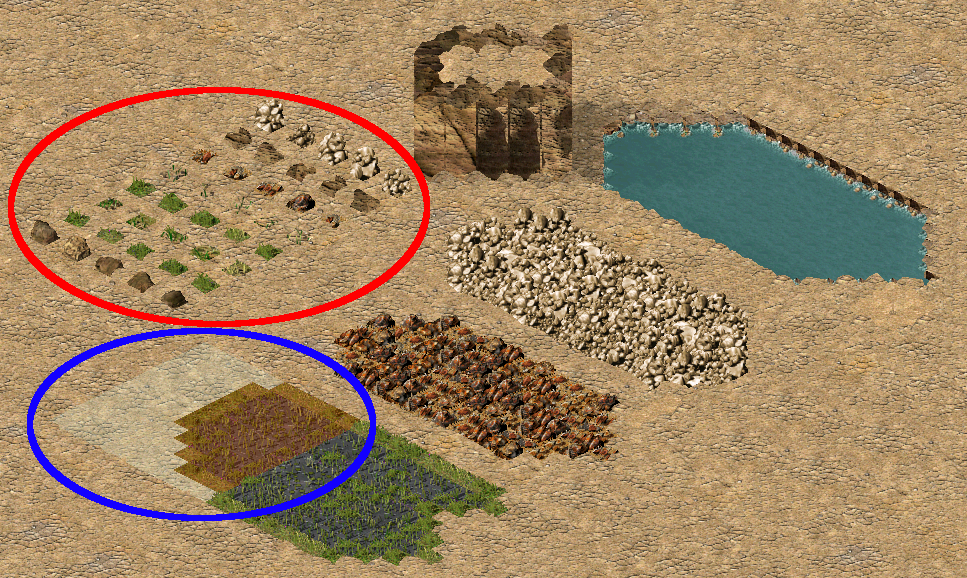
\includegraphics{strongholdtiles}
	\caption{Ukázka dlaždic ve hře Stronghold Crusader}
	\label{fig:tiletype}
\end{figure}

Na každé dlaždici může být postavena až na výjimky nejvýše jedna budova a stát nejvýše jedna jednotka. Při pohybu jednotek není tato vlastnost dodržována, lze tedy jednotky přesouvat přes dlaždice na kterých již jiná jednotka stojí. 

Naše platforma bude podporovat rozšířenější verzi tohoto druhu mapy, ve které nebudeme vynucovat limity na počty jednotek a budov na jedné dlaždici. Tato omezení budou přenechána pro implementaci tvůrcem her využívajících naší platformu a bude vytvořeno rozhraní pro co nejjednodušší implementaci těchto limitů. 

\todo[Další druhy]{popsat další druhy implementací}

Naše platforma bude podporovat mapu s těmito vlastnostmi:
\begin{itemize}
	\item[M1:] Terén rozdělený na čtvercové dlaždice.
	\item[M2:] Dlaždice s různou výškou.
	\item[M2:] Dlaždice různých typů.
	\item[M3:] Možnost dotazovat se na jednotky nacházející se na dlaždici.
	\item[M4:] Možnost dotazovat se na budovy postavené na dlaždici.
\end{itemize}
\subsection{Jednotky}
\label{sec:jednotky}
Jednotky jsou základním nástrojem hráče pro boj s nepřítelem. Pohybem po mapě, poškozováním ostatních jednotek a ničením budov jednotky umožňují hráči vést souboj s protivníkem, získat strategickou výhodu a následně vyhrát hru. 

\subsubsection{Pohyb}
Hlavním odlišujícím prvkem jednotek od budov je jejich schopnost pohybu. Pohyb jednotky je určen jejím typem, kde každý typ jednotek může procházet jinými typy terénu, pohybovat se nad terénem, na vodě či pod vodou. Naše platforma bude podporovat pohyb jednotek kdekoli nad terénem, navíc bude tvůrcům poskytnuta komponenta umožňující chůzi po terénu, neboť je to nejčastější způsob pohybu. 

Pohyb jednotek je nejčastěji řízen hráčem, ať už na úrovni příkazů jednotlivým jednotkám, tak na úrovni slučování jednotek do skupin a ovládání těchto skupin. Naše platforma bude umožňovat jak ovládání jednotlivých jednotek, tak celých skupin. Dále umožníme vývojáři přidat složitější ovládání, například slučování do permanentních formací a následné ovládání těchto formací. 

\todo{obrazek}
V některých hrách existují také jednotky, které se mohou své schopnosti pohybu vzdát a stát se budovu, buď dočasně, nebo trvale. Příkladem takovéto jednotky/budovy mohou být budovy Nočních elfů ze hry Warcraft 3 \citep{site:warcraft3nightelfs}. Tyto entity jsou stavěny jako budovy, tedy jsou umístěny do světa a postaveny jednotkou, stejně jako u všech ostatních ras. Následně je ale hráči umožněno, pomocí speciální ability těchto budov, změnit je dočasně na jednotky a pohybovat s nimi či je dokonce použít pro boj. V tomto módu ale ztrácí všechny funkce budov, tedy není možné je použít pro sběr surovin či produkci jednotek. Následně je možné znovu je zakořenit, čímž získávají zpět své funkce budovy.  Naše platforma by měla takovéto jednotky/budovy také podporovat. 

\subsubsection{Umělá inteligence}

Ve velké části RTS her jsou jednotky schopny do určité míry autonomního rozhodování bez zásahu hráče, od střelby na cíl, který se ocitne v jejich dostřelu, po vyhledání krytu, pokud jsou pod palbou. 

Jako příklad jednoduché umělé inteligence jednotek můžeme vzít hry Starcraft a Warcraft od společnosti Blizzard. Zde se jednotky chovají velice předvídatelně, splňují přesně hráčovi rozkazy a nedělají nic navíc, což umožnilo hře Starcraft II vytvořit jednu z prvních masivních e-sport scén na světě. \citep{site:gamasutra01}


\todo{obrazek s chovanim}
Dobrým příkladem jednotek s vysokou autonomií je série Company of Heroes, kde jednotky automaticky vyhledávají krytí, rozutečou se, pokud jsou pod palbou dělostřelectva, a v případě příliš velkých ztrát utečou z boje. Tato autonomie má ale svou cenu, a to v nepředvídatelnosti chování jednotek. Při jednoduché umělé inteligenci jednotek je hráč schopen předvídat jejich chování a využít ho pro svůj prospěch. Naopak při složité umělé inteligenci, jako právě v případě Company of Heroes, je hráč často nucen provést více pokusů při vydávání rozkazu, protože není schopen jednoduše odhadnout chování jednotky. Tato skutečnost činí hry často realističtější, protože simuluje chování reálných vojáků, kteří rozkaz interpretují a implementují podle svého, není ale vhodná pro souboje více hráčů, a už vůbec né více hráčů na profesionální úrovni.

Platforma bude umožňovat vykonat libovolný kód v rámci každého výpočtu stavu každé jednotky, bude tedy pouze na vývojáři, zda se budou jednotky chovat jednoduše a předvídatelně, nebo zda budou vykonávat složité, avšak nepředvídatelné úkony bez hráčova vědomí. Pro ulehčení vývoje bude platforma poskytovat předpřipravené komponenty, umožňující základní úkony jako střelbu na cíl, pohyb po mapě a útok na blízko.

\subsubsection{Produkce}

Jednou z vlastností definujících RTS hry je možnost produkce nových jednotek. Existuje několik systémů produkce jednotek, úzce svázaných se systémem surovin v dané hře. (viz. \ref{sec:suroviny})  Od kontinuální produkce, kde hráč zvolí produkované jednotky a suroviny jsou spotřebovávány v průběhu produkce, po diskrétní produkci, kde hráč musí vlastnit všechny suroviny potřebné pro výrobu dané jednotky při začátku produkce a všechny suroviny jsou odečteny v jeden okamžik. Kontinuální systém umožňuje hráči naplánovat produkci armády v předstihu, i když v daném okamžiku nevlastní dostatečné suroviny. Naopak při diskrétní produkci je hráč nucen čekat do chvíle, kdy má všechny suroviny, a až poté může začít s produkcí. Naše platforma se pokusí podporovat oba systémy. Bude záležet pouze na tvůrci hry, jak se k surovinám a produkci jednotek zachová a který z těchto systémů bude implementovat.

Počet jednotek je často limitován, jak pro účely vyvážení hry, tak pro omezení zátěže hardwaru. Z hlediska vyvážení síly jednotek umožňuje limit na počet jednotek předejít tzv. ``Zergu'', kdy hráč vytvoří obrovské množství levných jednotek, které následně převálcují jakýkoli odpor. Z hlediska hardwarové náročnosti je účel limitu vcelku zřejmý, protože každá jednotka zabírá určité množství paměti a výpočetního výkonu. Stronghold Crusader omezuje počet jednotek na 1000 pro každého hráče. Toto omezení se jeví především jako limit na hardwarovou náročnost hry. Naše platforma žádné explicitní limity nestanovuje, avšak v uživatelské dokumentaci pro vývojáře budeme silně doporučovat stanovení limitů na počet budov, jednotek a projektilů. Za tímto účelem umožníme vývojáři při vytvoření každé jednotky, budovy či projektilu učinit rozhodnutí, zda je vytvoření možné a případně toto vytváření zrušit. 

Hráč často začíná s malým počtem jednotek, jejichž účelem je zamezit tzv. ``Rush'' strategii, ve které je cílem vytvořit co nejrychleji co možná nejvíce levných jednotek a zničit nepřítele ještě před tím, než je schopen začít produkovat své jednotky. Ve hře Stronghold Crusader hráč začíná každou hru s několika lučišníky a kopiníky, jejichž počet je určen v nastavení před začátkem hry. Toto bude v naší platformě umožněno přidáváním jednotek v rámci editace mapy, případně bude tvůrce hry schopen umožnit hráči určit počty jednotek před začátkem hry pomocí grafických elementů v uživatelském rozhraní a následně při začátku hry vytvořit požadované množství jednotek. Tyto jednotky bude poté hráč vlastnit již na počátku hry.

\subsubsection{Boj}

V drtivé většině RTS her mají jednotky tzv. ``hit pointy'', zkráceně \textit{HP}, které určují počet zásahů, které může jednotka obdržet než bude zabita. S každým zásahem jsou poté tyto \textit{HP} odečítány a v okamžiku, kdy je jednotka poškozena na 0 \textit{HP} je zabita. Naše platforma bude tento systém samozřejmě podporovat, ale nebude ho nijak explicitně vyžadovat, bude tedy tvůrci umožněno použít jakýkoli jím implementovaný systém. 

Jednotky mohou obdržet poškození z mnoha zdrojů, nejčastěji však útokem z blízka (tzv. \textit{meele}) či z dálky (tzv. \textit{ranged}). Útok na blízko je omezen dosahem, rychlostí útoků a velikostí uděleného poškození. Naše platforma bude podporovat komponentu poskytující útoky na blízko právě s těmito parametry. Útok na dálku lze rozdělit do dvou typů, tzv. \textit{hit-scan} a \textit{projektily}. První typ je reprezentován například laserovými zbraněmi, které v okamžiku výstřelu urazí celou vzdálenost, dokud nenarazí na terén či nějakou entitu (budovu či jednotku). Druhý typ v okamžiku výstřelu vytvoří projektil, který se v průběhu času pohybuje herním světem, dokud také nenarazí na terén či nějakou entitu. Naše platforma bude podle předlohy Strongholdu Crusader podporovat především projektilové útoky. Za tímto účelem bude vytvořena komponenta umožňující střelbu projektilů, dále projektily samotné, simulace jejich letu a především možnost výpočtu pro střelbu na pohyblivý cíl. Hit-scan útoky nebudou přímo podporovány, mělo by však být umožněno tvůrci hry tento typ útoků implementovat manuálně.

\subsubsection{Shrnutí požadavků}
Naše platforma bude podporovat jednotky s těmito vlastnostmi:
\begin{itemize}
	\item[J1:] Pohyb jednotek volně kdekoliv nad terénem.
	\item[J2:] Podpora pohybu po terénu.
	\item[J3:] Ovládání jednotek a skupin jednotek.
	\item[J4:] Rozšiřitelnost o složitější ovládání.
	\item[J5:] Podpora jednoduché i složité umělé inteligence v podobě vykonání libovolného kódu.
	\item[J6:] Podpora diskrétní i kontinuální produkce jednotek.
	\item[J7:] Přidávání jednotek při editaci mapy.
	\item[J8:] Přidávání jednotek při startu hry.
	\item[J9:] Podpora systému hit-pointů.
	\item[J10:] Útoky na blízko i na dálku.
	\item[J11:] Projektily.
\end{itemize}

\done
\todo[Přeuspořádat]{Lépe uspořádat sekci o budovách}
\subsection{Budovy}
\label{sec:budovy}
Stavba budov představuje jednu z hlavních prezentací hráčovi strategie. Podle postavených budov lze často vcelku přesně odhadnout, jakou strategii hráč zvolil, čímž je umožněno nepřátelům reagovat a adaptovat svou strategii odpovídajícím způsobem. 
\todo[Reference]{Reference na rock-paper-scisors}
Při volbě strategie lze ale narazit na problém, kdy je hráč nucen zvolit svou strategii před tím, než nalezne protivníky a tedy před tím, než může vidět jejich strategii. Tento problém je velmi výrazný při tzv.  ``rock-paper-scisors'' strategiích, kde strategie 1 poráží strategii 2, strategie 2 poráží strategii 3 a strategie 3 poráží strategii 1. V tuto chvíli hra degeneruje v loterii, zda hráč náhodně vybere správnou strategii porážející tu vybranou nepřítelem.\citep{book:gamefund} Jedním z řešení tohoto problému je co nejmenší rozdíl v síle prvních úrovní technologie, což umožní hráčům reagovat a změnit svoji strategii před tím, než je rozdíl mezi jejich silami neúnosně velký. \citep{site:oxeye03} Dalším možným řešením, použitým ve Stronghold Crusader, je neskrývat před hráčem nepřítelovu strategii. Toto řešení lze použít v různé míře, od odhalení nepřátelských budov po úplné odkrytí celé mapy, tedy pozice všech jednotek i budov, ať už přátelských, nepřátelských či neutrálních. Naše platforma použije toto poslední řešení, kdy budeme hráč vidět všechny jednotky a budovy všech hráčů.

Budovy mají ve hrách mnoho funkcí, mezi které patří například:
\begin{itemize}
	\item Produkce jednotek
	\item Vylepšování jednotek
	\item Produkce surovin
	\item Uskladnění surovin
	\item Obrana
	\item Stavba budov
	\item Zkoumání technologií
\end{itemize}


Naše platforma se pokusí co nejvíce zjednodušit implementaci těchto funkcí poskytnutím programátorského rozhraní pro umístění budov a jednotek do herního světa, přidání a odebrání surovin hráči či střelbu projektilů. Dále umožníme tvůrci her přístup ke grafickému rozhraní, do kterého bude možné umístit okna, tlačítka a další elementy, které následně použitím programátorské rozhraní budou schopné implementovat všechny zmíněné funkce budov.  

Jak již bylo řečeno v sekci o jednotkách \ref{sec:jednotky}, naše platforma bude nechávat volbu mezi kontinuální a diskrétní produkcí jednotek na tvůrci hry. Budeme se tedy snažit do co největší míry podporovat oba tyto způsoby. 

\subsubsection{Obrana}

Obrana bude podporována v podobě komponent, které umožní budovám jak útok na blízko, jako v případě pastí ve hře Stronghold Crusader, tak na dálku, jako například obranné věže ve hře Warcraft 3. 

Dále v rámci funkce obrany umožňují v některých hrách budovy jednotkám pohybovat se po nich. Jak můžeme vidět na obrázku \ref{fig:unitsonbuildings} ze hry Stronghold Crusader, jednotky mohou být umístěny na hradbách, věžích, bránách či na tvrzi. Jak bylo řečeno v části o jednotkách, naše platforma bude umožňovat neomezený pohyb jednotkami, tedy i ve vzduchu, na budovách či skrz budovy. Protože se pohyb po budovách vyskytuje ve velkém množství RTS her, poskytne platforma možnost rozšíření terénu o plochu budov a komponentu umožňující chůzi po těchto plochách.

Umístění na budovách poskytuje jednotkám ochranu před nepřátelskými jednotkami útočícími na blízko, které se musí nejdříve dostat do blízkosti cíle, než zaútočí. 

V některých hrách, \todo[zkontrolovat]{zkontrolovat, ze opravdu Stronghold Crusader neni jednou z nich}kde bohužel Stronghold Crusader není jednou z nich, poskytuje vyvýšení nad terén jednotkám větší dostřel. Tento efekt nemusí být omezen pouze na vyvýšení pomocí budov, ale lze ho dosáhnout už při rozdílných výškách terénu, na kterém je umístěn střelec a jeho cíl, obecněji na rozdílu výšky pozice střelce a cíle, pokud se střelec nemusí pohybovat přímo po terénu. Naše platforma bude podporovat realistické chování projektilů splňující tuto vlastnost. 

\done
\todo{zničitelnost}
\done
\todo{různé druhy poškození}

Budovy, podobně jako jednotky, mají ve většině her určitý počet tzv. ``hit pointů'', které určují počet zásahů, které může budova obdržet před tím, než bude zničena. Navíc oproti jednotkám mohou budovy často obdržet poškození pouze od omezené podmnožiny jednotek, nejčastěji pouze obléhacích strojů. Stejně jako u jednotek přenecháme systém poškození na tvůrci hry. Naše platforma pouze umožní budově reagovat na zásah projektilem či zbraní, ať už snížením svých \textit{HP}, nebo ignorováním daného útoku v případě že přišel od jednotky či projektilu, který danou budovu nemůže poškodit.


\subsubsection{Stavba budov}
\done
\todo{restrikce na umístění}
Budovy mají často restrikce, které je hráč nucen splnit před stavbou budovy. Tyto restrikce mohou sahat od reliéfu a typu terénu, přes existenci jiných budov ve stejném místě, po vlastnictví určitého množství surovin či typu jednotek. Naše platforma umožní tvůrci před stavbou budovy zjistit stav všech těchto typů restrikcí a případně vetovat stavbu budovy. 

Jednou z restrikcí je výzkum určité technologie či stavba určité předcházející budovy\ref{sec:vyzkum}. Tímto způsobem jsou budovy uspořádány do postupně se zlepšujících úrovní, které hráč v průběhu času odemyká. Každá z úrovní obsahuje řadu rozdílných budov, umožňujících zvolit různé strategie. Platforma bude umožňovat tvůrci postupné zpřístupňování budov a jednotek, čímž bude tvůrce schopen implementovat postupné zkoumání nových technologií.

Existující hry využívají několik možností, jak hráči poskytnout zpětnou vazbu o splnění restrikcí při stavbě budovy. Jednoduší možností, použitou ve hře Stronghold Crusader, je zobrazení půdorysu v různých barvách podle splnění restrikcí. Další, složitější možností je zobrazení průhledného či jinak upraveného modelu budovy na místech, kde ji nelze postavit.  Naše platforma bude podporovat jednoduší způsob, tedy zobrazení půdorysu budovy v různých barvách podle požadavků tvůrce hry.

\subsubsection{Shrnutí požadavků}

Naše platforma bude podporovat tyto vlastnosti:
\begin{itemize}
	\item[B1:] Stavbu budov v herním světě.
	\item[B2:] Komponenty pro útok budov na blízko i na dálku.
	\item[B3:] Rozšiřitelnost dostupného terénu v herní mapě o prostor na budovách.
	\item[B4:] Podpora zvýšení dostřelu při umístění jednotky na vyvýšený terén, například budovu.
	\item[B5:] Stavba budov při editaci mapy.
	\item[B6:] Stavba budov při startu hry.
	\item[B7:] Podpora systému hit-pointů.
	\item[B8:] Tvůrcem definované reakce na obdržení zásahu budovou.
	\item[B9:] Zobrazení půdorysu v různých barvách pro zpětnou vazbu splnění restrikcí.
	\item[B10:] Kontrolu požadavků při stavbě budovy.
	\item[B11:] Přístup ke grafickému rozhraní, možnost zobrazení elementů hráči.
\end{itemize}


\subsection{Suroviny}
\label{sec:suroviny}
``Resource management'', tedy management surovin, je přítomný ve všech hrách žánru RTS již od jeho vzniku. Od koření v Dune II, přes zlato a dřevo ve Warcraft 3, po všechny typy surovin ve hře Stronghold, získávání surovin je jednou z hlavních motivací konfliktu v RTS hrách. 

Systémy surovin lze rozdělit podle způsobu získávání a počtu typů surovin.

Podle způsobu získávání můžeme systém surovin rozdělit na
\begin{enumerate}
	\item Aktivní získávání surovin
	\item Pasivní získávání surovin
\end{enumerate}

Při aktivním získávání surovin existuje ovladatelná herní entita, která svým pohybem mezi pozicemi na mapě přináší suroviny. Tento pohyb může být ovládán hráčem, ale nejčastěji dokáže pracovat jednotka samostatně. Příkladem může být Warcraft 3 \citep{site:warcraft3}, kde speciální jednotky získávají dřevo a zlato přenášením z lesů/dolů do hráčovy hlavní budovy. Při pasivním získávání přibývají suroviny bez akcí entit, pouze díky vlastnictví určité části mapy nebo druhu budovy. Zdroj bývá nekonečný nebo skoro nekonečný, poskytující suroviny do obsazení nebo zničení zdroje. Každý z těchto stylů podporuje jinou strategii kontroly mapy.

Naše platforma bude podporovat jak pasivní, tak aktivní získávání surovin. Bude pouze na tvůrci, v jakém okamžiku budou suroviny přičteny, ať už v závislosti na čase nebo na pohybu určitých jednotek. 

\subsubsection{Shrnutí požadavků}

Naše platforma bude podporovat tyto vlastnosti:
\begin{itemize}
	\item[S1:] Podporovat aktivní i pasivní získávání surovin.
	\item[S2:] Poskytnout rozhraní pro přidání a odebrání surovin hráči.
\end{itemize}

\subsection{Vývoj technologií}
\label{sec:vyzkum}
Volba vyzkoumaných technologií důležitou součástí strategické části RTS her. 

Technologie jsou často uspořádány ve stromové struktuře či orientovaném acyklickém grafu (DAG), kde vyzkoumání technologie v rodičovském uzlu odemyká technologie následujících uzlech. Příklad takového uspořádání můžeme vidět v ukázce ze hry \emph{Civilisation V}\citep{site:civ5}\ref{fig:civ5techtree}, kde vidíme počátek stromu technologií. V této hře jsou technologie uspořádány do DAGu, začínajícího v jednom kořeni. Můžeme vidět žluté vrcholy, značící vyzkoumané technologie, dále zelené vrcholy, značící technologie, které mají splněné všechny předky a mohou být vyzkoumány, černé technologie, které bude možné začít zkoumat po odemčení všech předků, a nakonec červené technologie, značící technologie v dalším věku. Dále můžeme vidět hrany spojující závislé technologie. 

Další možné uspořádání je několik disjunktních stromů technologií, kdy je hráč nucen zvolit jeden z těchto stromů. 
Toto uspořádání můžeme vidět ve hře Company of Heroes \citep{site:COH}, kde jsou hráči dostupné tři vzájemně výlučné cesty, každá zaměřená na jinou oblast boje. Každá z těchto cest je dále rozdělena na dvě větve postupně se zlepšujících technologií.

Každé větvení v grafu technologií představuje možné rozhodnutí hráče, kterou z větví se hráč vydá a které technologie odemkne. Toto rozhodnutí jsou jedním z hlavních projevů hráčovi strategie.

Vyzkoumání technologie může mít mnoho různých efektů. Nejčastějším efektem bývá odemknutí nového typu jednotek nebo budov. Další možností je změna vlastností již vlastněných jednotek nebo budov. V neposlední řadě pak může vyzkoumání technologie odemknout nové schopnosti nebo kouzla, které hráč může následně použít při taktických soubojích. 

\begin{figure}[h]	
	\centering
	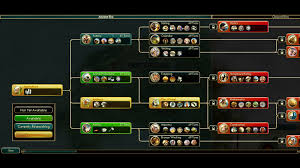
\includegraphics{civ5_tech_tree}
	\caption{Výřez stromu technologií ze hry Civilisation V}
	\label{fig:civ5techtree}
\end{figure}


Explicitní strom technologií, viditelný na \ref{fig:civ5techtree}, se v RTS hrách vyskytuje spíše výjimečně. Nejčastěji je odemykání nových typů jednotek a budov umožněno stavbou určitého typu budovy nebo dosažení určitého stupně vylepšení již existující budovy. Jako příklad můžeme vzít Warcraft 3 \citep{site:warcraft3}, kde závislosti budov na stupních vylepšení a existenci jiných budov tvoří strom technologií. Graf tvořený těmito závislostmi můžeme vidět na obrázku \ref{fig:warcrafttechtree}. Zde vidíme stupně vylepšení budov, reprezentované šedými šipkami, a závislosti budov na ostatních budovách a stupních jejich vylepšení. Aby byl hráč schopen postavit budovu, musí vlastnit všechny budovy na kterých je tato budova závislá v požadovaném nebo lepším stupni vylepšení. Ve hře je tento graf reprezentován požadavky zobrazenými při najetí myší na ikonu zamčené budovy.

\begin{figure}[h]	
	\centering
	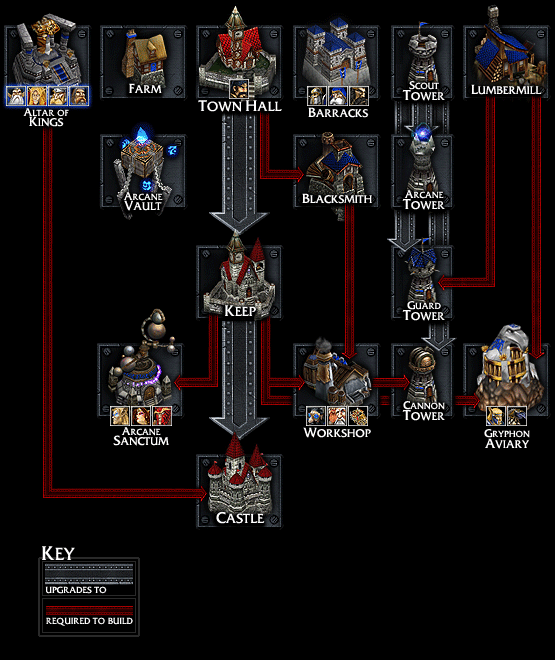
\includegraphics{warcraft_tech_tree}
	\caption{Budovy a závislosti mezi nimi tvořící obdobu stromu technologií ve hře Warcraft 3}
	\label{fig:warcrafttechtree}
\end{figure}

Jak bylo řečeno v sekci o budovách \ref{sec:budovy}, naše platforma bude umožňovat tvůrci postupné odemykání budov a jednotek, což umožní tvůrci her implementovat výzkum nových technologií. Pro technologie měnící vlastnosti typů jednotek bude pouze na tvůrci, aby změnil logiku hry a chování umělé inteligence v závislosti na vyzkoumaných technologiích.

\subsubsection{Shrnutí požadavků}

Naše platforma bude podporovat tyto vlastnosti:
\begin{itemize}
	\item[T1:] Umožnit postupné odemykání budov a jednotek.
	\item[T2:] Změny chování a vlastností jednotek v průběhu hry.
\end{itemize}

\section{Uživatelé}
V předešlé sekci jsme popsali druh her, který bude naše platforma podporovat. V této sekci popíšeme požadavky na chování platformy z pohledu všech druhů našich uživatelů.

\subsection{Tvůrci her}
Prvním druhem uživatele budou tvůrci her, používající naši platformu pro zjednodušení své práce a vyřešení problémů opakujících se ve většině RTS her. Tvůrce samozřejmě nemusí být pouze jeden člověk, vzhledem ke složitosti RTS her existuje při jejich tvorbě mnoho rolí, které požadují velmi různorodé schopnosti a mohou být plněny více lidmi. Příkladem rolí může být 3D umělec tvořící modely a animace, producent hudby, tvůrce umělé inteligence, programátor herní logiky a nakonec člověk, který toto vše integruje dohromady.

\subsubsection{Programátor}
Naším hlavním cílem je umožnit tvůrcům umělé inteligence a programátorům herní logiky použít všechny jazyky .NET Frameworku, především C\#, pro jejich práci. Z programátorského pohledu bude naše platforma sloužit jako knihovna poskytující tyto funkce:

\begin{enumerate}
	\item Udržovat aktuální stav hry a umožňovat dotazy na tento stav.
	\item Vytvářet nové jednotky, budovy a projektily.
	\item Registrovat si metody, které budou zavolány při určitých událostech v průběhu hry.
	\item Upravovat terén.
	\item Vykreslovat terén, jednotky, budovy, projektily a grafické rozhraní.
	\item Ukládat a načítat stav hry.
	\item Implementace pro základní problémy jako pohyb po terénu, let projektilů, výpočet úhlu střelby projektilů. \todo{more}.
	\item Ovládání kamery.
\end{enumerate}

Protože implementace vykreslování a grafického rozhraní by byla nad rámec jedné bakalářské práce, využije naše platforma pro tyto účely existující herní engine UrhoSharp. Pro programátory následně  poskytneme přístup k relevantním částem UrhoSharp enginu.

Platforma bude poskytovat ovládání kamery v několika módech. Tato funkcionalita bude potřebná již pro implementaci editoru, poskytneme ji tedy i tvůrcům her. Prvním módem bude klasická RTS top-down kamera, jakou můžete vidět na ukázce ze hry Company of Heroes \ref{fig:COHCam}. V této hře je oproti jiným starším RTS hrám jako Warcraft 3 nebo Age of Empires 3 s kamerou možné rotovat a přibližovat, což nám přijde jako velice atraktivní. Toto bychom rádi podporovali i v naší platformě. Druhým módem kamery bude tzv. ``free-float'', kdy kamera volně ``létá'' nad terénem. Třetím módem bude sledování jednotky, kdy se kamera bude chovat jako v prvním módu, její pohyb bude ale řízen pohybem jednotky.

\subsubsection{Moddeři}

Pro integraci vytvořených jednotek, budov, dlaždic a jejich modelů, textur a logiky umožní naše platforma vytvořit \emph{balíček}, obsahující vše vytvořené programátory a umělci.  Tento balíček poté platforma umožní přidat a načíst v libovolné instalaci platformy.

Platforma bude také sloužit jako editor úrovní, které budou využívat logiku, jednotky, budovy a typy terénu dodané pomocí balíčků. Vytvořené úrovně bude následně možné uložit zpět do balíčku a distribuovat spolu s balíčkem do dalších instancí naší platformy.

Pro editaci mapy poskytne platforma několik základních nástrojů a umožní tvůrcům modifikovat nástroje či přidávat své vlastní. Základní nástroje by měli umožnit editaci terénu mapy (změnu typu terénu na všechny tvůrci definované typy a editaci výšky dlaždic) a přidávání všech druhů jednotek a budov do mapy.

Formát ukládání úrovní bude definován otevřeně pomocí prostředků nezávislých na programovacím jazyce, čímž chceme umožnit tvorbu separátních editorů map produkujících úrovně v námi používaném formátu.

\subsection{Hráči her}
Z pohledu hráče se bude platforma chovat jako instalovatelná aplikace, která hráči umožní za běhu přidávat balíčky a následně využít jejich obsah.

Při běhu platforma umožní plný přístup k nastavení UrhoSharp enginu, tedy k nastavení rozlišení, Vsync, triple buffer a dalších. Dále umožní správu balíčků, tedy přidávání, odebírání a spouštění. Při spuštění balíčku umožní platforma hráči výběr z existujících map, jak pro hraní, tak pro editaci. Dále platforma umožní vytvoření a editaci úplně nové mapy.

Při tvorbě nové mapy či editaci existující mapy mít bude hráč přístup ke všem jednotkám, budovám a typům terénu, ke kterým mu dají editační nástroje specifikované tvůrcem balíčku přístup. Následně bude hráči umožněno mapu uložit, a to přepsáním zdrojové mapy, kterou hráč načetl k editaci, nebo vytvořením nové mapy pod novým jménem.

\section{Ukázková hra}
\label{sec:showcasedef}

Pro ukázku bude vytvořen balíček s jednoduchou hrou demonstrující možnosti naší platformy. Ukázková hra bude zároveň sloužit jako referenční příklad použití naší platformy.

Ukázková hra bude obsahovat několik jednotek, demonstrujících tyto vlastnosti:
\begin{enumerate}
	\item Jednoduchou a složitou umělou inteligenci
	\item Plně automatické jednotky, neovladatelné hráčem
	\item Jednotky útočící na dálku
	\item Jednotky útočící na blízko
	\item Aktivní získávání surovin
	\item Pohyb po terénu
	\item Pohyb nad terénem (létání)
	\item Rozdílnou rychlost pohybu různých jednotek
	\item Rozdílnou přístupnost částí mapy pro různé jednotky
	\item Pohyb po budovách
\end{enumerate}

Demonstrovanými vlastnostmi budov budou:
\begin{enumerate}
	\item Restrikce na místo stavby
	\item Neprostupnost budov pro některé jednotky
	\item Produkce surovin budovami
	\item Přidání plochy nebo části plochy budovy jako přístupný terén pro určité typy jednotek
\end{enumerate}

Jako obecné vlastnosti bude ukázková hra demonstrovat:
\begin{enumerate}
	\item RTS mód kamery
	\item Volný pohyb kamery
	\item Sledování jednotky kamerou
	\item Tvůrcem definované prvky v uživatelském rozhraní
	\item Minimapu
\end{enumerate}

Balíček obsahující ukázkovou hru bude demonstrovat tyto vlastnosti:
\begin{enumerate}
	\item Tvorbu vlastních úrovní za použití jednotek, budov a typů terénu obsažených v balíčku.
	\item Ukládání a načítání hry.
\end{enumerate}

\section{Cíle práce}
\label{sec:cileprace}
Cílem této práce je vytvořit platformu pro vývoj 3D RTS her pro jednoho hráče za použití herního enginu UrhoSharp, umožňující vývojářům vytvářet hry jako separátně 
distribuované balíčky, které bude poté koncový uživatel schopen přidat do naší platformy nainstalované na uživatelově počítači a použít je pro hraní dodaných úrovní či tvorbu svých vlastních.

Při tvorbě hry bude umožněno tvůrci použít jazyky frameworku .NET  pro vytvoření Umělé inteligence jednotek, budov a nepřátelských hráčů, pro vytvoření další logiky hry a pro přidání nástrojů do editoru map. 

Požadované vlastnosti platformy:
\begin{enumerate}
	\item Podporované vlastnosti jednotek:
		\begin{enumerate}
			\item Pohyb jednotek (J1, J2)
			\item Ovládání jednotek (J3, J4)
			\item Umělá inteligence, definice chování (J5)
			\item Produkce jednotek (J6)
			\item Přidávání jednotek jako součást mapy (J7, J8)
			\item Podpora systému hit-pointů (J9)
			\item Útoky na blízko i na dálku (J10, J11)
		\end{enumerate}
	\item Podporované vlastnosti budov:
		\begin{enumerate}
			\item Stavba budov v herním světě (B1, B9, B10)
			\item Podpora obraných budov (B2, B4)
			\item Rozšiřitelnost dostupného terénu o plochu budov (B3)
			\item Přidávání budov jako součásti mapy (B5, B6)
			\item Zničitelnost budov (B7, B8)
			\item Produkce jednotek, surovin, stavba budov pomocí budovy (B11)
		\end{enumerate}
	\item Podpora surovin:
		\begin{enumerate}
			\item Přidávání a odebírání libovolného počtu surovin (nejen celočíselných) (S1, S2)
		\end{enumerate}
	\item Podpora výzkumu technologií:
		\begin{enumerate}
			\item Umožnit postupné odemykání dostupných jednotek a budov, umožnit změny chování jednotek za běhu (T1, T2)
		\end{enumerate}
	\item Vlastnosti pro tvůrce balíčků:
		\begin{enumerate}
			\item Platforma musí umožňovat přidávání balíčků za běhu, obsahujících nové typy jednotek, budov,  dlaždic, projektilů a hráčů spolu s jejich modely, texturami a AI.
			\item Platforma musí umožňovat použití přidaných balíčků pro tvorbu map a uložení vytvořených map do balíčku použitého pro jejich tvorbu.
			\item Editor map musí být rozšiřitelný o nástroje z balíčku.
			\item Herní grafické rozhraní musí umožňovat tvůrci přidávat vlastní okna, tlačítka a další prvky.
		\end{enumerate}
	\item Vlastnosti pro koncového hráče:
		\begin{enumerate}
			\item User interface pro stolní počítače, umožňující vybírání balíčků, map a oponentů, dále načítání a ukládání her, a nastavování zobrazení hry.
			\item Herní user interface musí obsahovat minimapu, poskytující hráči přehled o větší části mapy než kterou vidí vlastní kamerou.
			\item Ovládání kamery umožňující klasický top-down pohled, volné poletování kamery po mapě a následování jednotky.
			\item Ukládání a načítání hry.
		\end{enumerate}
\end{enumerate}

\chapter{Analýza}
V první kapitole jsem specifikovaly náš cíl, tedy implementaci platformy nad enginem UrhoSharp umožňující tvorbu RTS her a jejich distribuci. V této kapitole popíšeme problémy při implementaci platformy a jejich možná řešení.

\section{Herní engine}
Jak jsme psali v Cílech práce (viz \ref{sec:cileprace}), naším cílem je vytvořit platformu za použití herního enginu UrhoSharp. ``UrhoSharp je multiplatformní 3D a 2D engine který může být použit pro tvorbu animovaných 3D a 2D scén za použití modelů, materiálů, světel a kamer''\citep{site:urhosharp}, jak říká úvodní stránka dokumentace enginu. Jak už název napovídá, UrhoSharp je .NET binding pro Urho3D engine \citep{site:urho3D}, což je opensource engine implementován v C++.

\todo{porovnání s dalšími enginy}

\section{Podporované platformy}
Jak bylo zmíněno v předešlé sekci, je námi používaný herní engine multiplatformní. Bohužel každá z platforem má určitá specifika a restrikce, jak obecně, tak v rámci enginu, které nás nakonec vedli k podpoře pouze platformy Windows. 

\subsection{Mobilní platformy}
Při implementaci pro mobilní platformy existuje několik problémů.
Herní engine sice mnohé rozdíly platforem odstraňuje, existují ovšem oblasti, které i při využití prostředků enginu vyžadují pro každou platformu různý design.

\subsubsection{Zobrazení a ovládání}
Na mobilních platformách je mnohem bližší vztah mezi GUI, tedy grafických uživatelským rozhraním, a ovládání. Oproti platformě PC je zde jediným možným vstupem dotyková obrazovka. GUI musí tedy sloužit jak pro zobrazení informací hráči, tak pro získání vstupu od hráče. Dalším rozdílem je velikost obrazovky, která je obecně mnohem menší než u jiných platforem. I přes to, že herní engine umožňuje tvorbu grafického rozhraní použitelného na všech platformách, tyto dva rozdíly nutí nás i tvůrce her k výrazně odlišnému návrhu rozhraní pro mobilní platformy. Engine Urho3D poskytuje separátní vývojové prostředí, které je možné použít pro definici uživatelského rozhraní a export této definice do XML souboru, který je poté možné načíst za běhu pro zobrazení specifikovaného uživatelského rozhraní. 

Oba tyto problémy nás vedou k separátní implementaci uživatelského rozhraní pro mobilní zařízení. Pro tuto implementaci jsme v naší práci připravily základní kostru, upustili jsme ovšem od konečné implementace z důvodu nedostatku času.

\subsubsection{JIT vs. AOT}
Dalším rozdílem, tentokrát s rozdílným chováním i mezi různými mobilními platformami, je jejich chování ke kódu aplikací. Jak víme, assembly pro platformu .NET či .NET Core obsahuje CIL kód, který je za běhu překládán do instrukční sady běžícího procesoru a následně vykonán. Tento systém se označuje jako ``\emph{Just in time}'' kompilace, zkráceně \emph{JIT}. Na systémech Windows, Linux, macOS či Android jsou .NET assembly spouštěny právě tímto způsobem. Oproti tomu systém \emph{iOS} zakazuje namapování stránek paměti zároveň pro zápis a pro vykonání, čímž znemožňuje jakoukoli JIT kompilaci. Z tohoto důvodu musí být všechny aplikace pro systém \emph{iOS} překládány tzv. ``\emph{Ahead of time}'',  zkráceně \emph{AOT}, tedy před tím, než jsou distribuovány k uživateli, přímo do instrukční sady cílového procesoru.\citep{site:aot} Tato skutečnost znemožňuje jednoduché nahrání assembly pomocí reflexe a nutila by nás k složitějšímu řešení. 
Tvůrce balíčku by musel své kódy přeložit pro všechny možné architektury, a naše platforma by se následně při běhu musela podle platformy, na které běží, rozhodovat, kterou z assembly nahrát. Toto je další důvod, proč jsme upustily od podpory systému iOS.

\subsubsection{Souborové systémy}
Přístup k souborům distribuovaným spolu s aplikací, v našem případě s naší platformou, se odlišuje několika způsoby. Prvním je jejich otevření, či vůbec nalezení. Na platformě Android je každá aplikace distribuována jako .apk soubor. Apk je zip archiv, obsahující všechny soubory naší aplikace, od kódu, přes assety, po preference. Tento archiv je přímo namapován do stromu souborového systému viditelného z naší aplikace. Bohužel .NET filesystem API nedokáže s tímto mapováním pracovat, tedy není možné ho využít pro čtení těchto souborů. Řešením je využití Xamarin.Android zabalujícího Android Java API, které s tímto archivem dokáže pracovat.

Toto nás nutí pro vyčlenění komponenty pro práci se soubory do zvláštní implementace pro každou platformu. 

Dalším problémem je, že oproti PC nelze do těchto souborů zapisovat, ani za použití jiného API. Toto není sice dobrý design aplikace ani na PC platformách, kde by data specifická pro daného uživatele měla být umístěna do adresáře jako MyDocuments/\$app na Windows nebo /home/\$USER/\$app, protože adresář, v kterém je aplikace nainstalovaná, může být pro většinu uživatelů namapován pouze pro čtení, ale při tvorbě jednodušších aplikací je vcelku obvyklé vytvářet soubory v currentDir a zapisovat do nich.


\subsubsection{Shrnutí}
Velká část problému popsaných v této části je řešitelná a tato řešení jsme u každého problému nastínili. Naše platforma bude obsahovat kostru těchto řešení, nebude je ovšem implementovat úplně, především kvůli nedostatku času. 

Některé problémy, jako například zákaz JIT kompilace na platformě iOS, jsou ovšem fatální pro myšlenku naší práce a byli jsme nuceni vyřadit tuto platformu i z možnosti budoucí podpory.


\subsection{Platformy stolních počítačů}
Naším hlavním cílem byla implementace naší platformy na operační systém Windows, především kvůli nejrozsáhlejší podpoře frameworku .NET, dále kvůli zřejmým výhodám uspořádání ovládání v podobě klávesnice a myši, a v neposlední řadě kvůli naší zkušenosti s tímto systémem.

Díky využití multiplatformního herního enginu a frameworku .NET by nemělo být složité v budoucnu rozšířit podporu na distribuce Linuxu a macOS. Kvůli rozsáhlosti práce ovšem nebude tato podpora v námi odevzdané implementaci.

\section{Formát a načítání dat}
Důležitou součástí implementace naší platformy je systém balíčků pro distribuci vytvořených her. Tyto balíčky obsahují všechny součásti hry, od modelů a textur, přes logiku a umělou inteligenci, po mapy a úrovně vytvořené tvůrcem hry. Všechny tyto součásti musí naše platforma být schopna načíst za běhu a použít jak pro tvorbu nových map, tak pro hraní již existujících.

\subsection{Základní struktura balíčku}
\todo[Rozdelit do subsekci]{Rozdelit do subsekci}
Pro implementaci načítání balíčků musíme definovat strukturu, kterou budou balíčky splňovat, a podle které bude platforma určovat typy souborů a jejich závislosti. 

První možností je založit strukturu balíčku na adresářové struktuře, kde každý balíček bude tvořen jedním adresářem obsahujícím další pevně specifikované podadresáře. Každý z podadresářů by obsahoval jeden z typů zdrojů, tedy 3D modely, textury, popis jednotek nebo skripty.

Pro popis typů jednotek, budov, projektilů, dlaždic a nepřátel jsme se inspirovali v existujících hrách, ať už Civilisation V nebo Kerbal Space Program, a využili jsme XML soubor pro definici závislostí. Dalšími možnostmi bylo využít formát JSON nebo dokonce definovat vlastní formát. Možnou výhodou formátu JSON je jeho expresivita, umožňující minimalizovat velikost souborů. Vzhledem k velikosti grafických dat jsme ovšem usoudily, že tato výhoda není dostačující pro volbu tohoto formátu. Pro formát XML jsme se rozhodli především kvůli vestavěné podpoře v platformě .NET a možnosti validace vůči schématu, která nám ulehčí od implementace vlastní validace. 

Toto rozdělení ovšem vedlo ke dvěma problémům. Prvním bylo velké množství malých XML souborů, jejichž správa by ...
Druhým problémem bylo přidávání balíčku do běžící hry. Hráč by mohl sice specifikovat adresář reprezentující balíček, následné ověření, zda je tento balíček korektní a lze ho nahrát nás nutí k procházení adresářové struktury, načítání mnoha souborů a k pokusům o jejich načtení a validaci.

Řešením bylo vytvořit centrální XML soubor, definující celý balíček. Všechny typy jednotek, budov, projektilů, nepřátel, logik úrovní, všechny úrovně obsažené v balíčku a další jsou popsány v tomto souboru. Následně všechny assety, tedy modely, textury či assembly mohou být specifikovány relativní cestou vůči adresáři obsahujícímu tento soubor. Tímto způsobem lze replikovat předchozí uspořádání, kde je každý typ assetů rozdělen do vlastního adresáře, ale navíc tento způsob umožňuje tvůrci balíčku specifikovat vlastní rozdělení a umístění assetů. Zároveň toto uspořádání ulehčuje přidání balíčku a ověření jeho korektnosti, kde stačí, aby uživatel zadal cestu k tomuto souboru, a pouhou validací XML souboru podle schématu lze ověřit správnost.

Tedy v konečném řešení je každý balíček reprezentován jedním XML souborem, který dále obsahuje relativní cesty, odkazující na zbylý obsah balíčku. Tento soubor má formát daný pevným schématem a tento formát je kontrolován při každém načítání. 

\subsection{Formáty assetů}
\subsubsection{3D assety}
Podporované formáty 3D assetů jsou limitovány námi používaným herním enginem. Urho3D, a tedy i UrhoSharp, používá Open Asset Import Library (Assimp) \citep{site:assimp}, open source knihovnu podporující uniformní načítání assetů z různých formátů do jednoho standardního formátu, definovaného touto knihovnou.
\subsubsection{Assembly}
Náš systém balíčků poskytuje tvůrcům možnost vytvořit vlastní kód, který následně naše platforma za běhu načítá a spouští. Tento proces nás vedl k použití reflection, a k metodám Assembly.LoadFile a Assembly.LoadFrom. Rozdíl mezi těmito metodami vychází z různých contextů, do kterých jsou assembly nahrávány. 

Existují tři/čtyři kontexty, do kterých jsou assembly nahrávány. Těmito kontexty jsou\citep{site:assemblyload}:
\begin{itemize}
	\item Default Load Context
	\item Load-From Context
	\item Reflection-only Context
	\item No Context
\end{itemize}

Reflection-only context slouží pro zkoumání assembly pomocí reflection a znemožňuje vykonání kódu nahraného do tohoto kontextu, proto je pro nás nezajímavý a dále ho nebudeme rozebírat.

Default Load Context je kontext, ve kterém je nahrána assembly naší aplikace a všechny její závislosti. Do tohoto kontextu lze manuálně nahrávat další assembly, pokud se tyto assembly nachází v GAC, applicationBase a PrivateBinPath. Assembly se zde identifikují jménem, které následně runtime hledá na všech zmíněných místech. Závislosti nahrávaných assembly jsou automaticky vyhledávány na těch samých místech.

Load-From Context je kontext, do kterého nahrává assembly metoda Assembly.LoadFrom. Do tohoto kontextu lze nahrát assembly specifikováním cesty, lze tedy nahrávat mimo GAC, applicationBase a PrivateBinPath. Závislosti jsou hledány v Default Contextu, případně v adresáři, ze kterého byla assembly nahrána a nakonec na zmíněných cestách pro nahrávání do Default Contextu.

No Context je využíván načítá  assemblies vygenerovaných pomocí reflection emit a Assembly.LoadFile. Navíc je to jediný způsob, jak načíst dvě verze té samé assembly. Pod pokličkou je vytvořen každé nahrané assembly zvláštní privátní kontext. Problémem tohoto kontextu je, že nejsou automaticky nahrávány závislosti. Tedy nezbývá nám nic jiného než závislosti nahrát manuálně před načtením assembly nebo odchytit AssemblyResolve event.

V naší platformě používáme Assembly.LoadFrom, které řeší všechny naše problémy. Díky načítání závislostí ze zdrojového adresáře assembly mohou tvůrci her přibalit jimi používané knihovny do balíčku a ty budou následně při použití automaticky načteny.

\todo{odnačítání assemblies}
Problém může nastat, pokud dva nezávislé balíčky budou používat dvě různé verze té samé knihovny, které budou načteny z jejich adresáře. Pro vyřešení tohoto problému by bylo nutné naimplementovat zahazování načtených assembly.

\subsection{Formát uložených úrovní}
Ukládáním úrovně rozumíme serializaci aktuálního stavu hry a uložení takto serializovaných dat do souboru.

Pro serializaci jsme měli několik požadavků. Hlavním z nich byla otevřenost schématu serializovaných dat. Účelem tohoto požadavku je umožnit tvorbu nezávislých editorů úrovní, importujících a exportujících náš formát dat. Dalším požadavkem byla minimalizace velikosti serializovaných dat, pro umožnění tvorby velkého množství úrovní a úložek hry. Spolu s předešlým požadavkem jde potom rychlost serializace a deserializace dat.

První požadavek splňují serializace do XML, specifikovaného pomocí XSD schématu, a binární serializace popsaná pomocí interface description language. Příkladem takové binární serializace je formát Protocol-buffers od společnosti Google. 

Druhý a třetí požadavek nás vedli k binární serializaci, která minimalizuje velikost dat a má nejrychlejší zpracování. Tímto jsme vybrali formát protocol buffers, který lze v jazyce C\# použít buď separátní specifikací message a následnou manuální serializací, nebo využitím knihovny Protobuf-net, která z anotací ve zdrojovém kódu generuje specifikaci message a  metody pro serializaci a deserializaci dat.

Bohužel náš graf scény byl natolik složitý, že serializace pomocí Protobuf-net začínala být příliš složitá. Vzhledem k tomu, že samy Protocol buffers nepodporují reference, nemá ani Protobuf-net velkou podporu referencí. Přesto že by nejspíš naše data šli serializovat pomocí Protobuf-net, rozhodli jsme se použít manuální specifikaci a serializaci, která nám dává větší kontrolu nad postupem serializace a konečným formátem dat. To nám navíc umožnilo rozdělit specifikace do separátních souborů podle logických závislostí, okomentovat tyto specifikace a případně distribuovat separátně. 


\section{Mapa}

\section{Pathfinding}
\chapter{Ukázková hra}
\chapter{Uživatelská dokumentace}
\chapter{Tvorba pluginů}
\label{sec:pluginmaking}
Pojmem \uv{plugin} v~naší platformě rozumíme .NET assembly nahranou platformou za běhu a~implementující chování úrovní, hráčů, jednotek, budov či projektilů. Pluginy jsou v~balíčku uloženy jako \texttt{.dll} knihovny, cílené pro .NET Framework 4.7.2. 

V~této části dokumentace popíšeme postup vytvoření takovéto knihovny. Její následné připojení do balíčku je popsáno v~předchozí části \ref{sec:packagemaking}.

Pro tvorbu balíčků je nutné využít knihovnu \texttt{MHUrho.dll}, poskytující přístup k předkům pluginů a dalším funkcím platformy. Tato knihovna je dostupná v přílohách práce \ref{sec:appendix}.

Platforma nijak neomezuje rozdělení pluginů pro různé herní prvky do různých knihoven. Lze tedy všechny pluginy shromáždit v~jedné knihovně, jak je to provedeno v~ukázkové hře, nebo je možné vytvořit více různých knihoven s~libovolným rozdělením pluginů.

Stejně jako v~předchozí části i~zde je velká část tvorby shodná pro různé druhy prvků. Celý proces proto popíšeme pouze v~části tvorby pluginu jednotky a~v~následujících částech uvedeme pouze rozdíly oproti této části.


\section{Vytvoření pluginu jednotky}
\label{sec:unittypeplugin}
V~této části popíšeme tvorbu typu jednotky. Tato jednotka bude mít tyto vlastnosti:

\begin{itemize}
	\item 3D model s~animacemi,
	\item pohyb po terénu přes omezenou množinu typů dlaždic,
	\item střelba na dálku za použití projektilů typu specifikovaného v~XML.
\end{itemize}

Jako první vytvoříme definici jednotky v~XML. Tento krok je popsán v~předchozí části \ref{sec:packagemaking}, nebudeme ho zde proto opakovat. Výsledné XML typu jednotky tedy bude takovéto:

\begin{lstlisting}[
	style=xml,
	morekeywords={unitType, assets,path,  assemblyPath, extension, cost, Wood, Gold, canPass, Sand, Xamarin, Grass, Water, iconTextureRectangle},
	emph={[1]name, ID, type, left, top, right, bottom}
]
<unitType name="Chicken" ID="3">
	<assets type="xmlprefab">
		<path>Assets/Units/Chicken/prefab.xml</path>
	</assets>
	<assemblyPath>ShowcasePackage.dll</assemblyPath>
	<extension>
		<cost>
			<Wood>0.2</Wood>
			<Gold>0.5</Gold>
		</cost>
		<canPass>
			<Sand/>
			<Xamarin/>
			<Grass/>
			<Water/>
		</canPass>
	</extension>
	<iconTextureRectangle left="0" top="200" right="100" bottom="300"/>
</unitType>
\end{lstlisting}

Hotovou jednotku můžete vidět v~ukázkové hře pod názvem \texttt{Chicken}.

\section{Plugin typu}
Prvním krokem je vytvoření dvou veřejných tříd, jedné reprezentující plugin typu a~druhé reprezentující plugin instance. 

Jako první vytvoříme třídu reprezentující plugin typu. Tato třída musí být veřejná a~dědit od třídy \texttt{UnitTypePlugin}, definované platformou. Takováto třída poté bude nalezena pomocí \texttt{Reflection} a~za běhu platformy načtena jako plugin daného typu.  

\begin{lstlisting}[
	style=csharp,
	emph={[1]ChickenType, UnitTypePlugin}
]
public class ChickenType : UnitTypePlugin {

}
\end{lstlisting}

Následuje implementace požadovaných vlastností a~metod třídy. Jako první přidáme vlastnosti \texttt{Name} a \texttt{ID}.

\begin{lstlisting}[
	style=csharp
]
public override string Name => "Chicken";
public override int ID => 3;
\end{lstlisting}

Tyto vlastnosti jsou používány pro nalezení pluginu pro daný typ. Hodnoty \texttt{Name} a \texttt{ID} se tedy musí shodovat s~hodnotami uvedenými v~atributech \texttt{name} a \texttt{ID} v~XML definici typu.

Dále platforma po všech typových pluginech požaduje implementaci tří hlavních metod:

\begin{enumerate}
	\item \texttt{Initialize},
	\item \texttt{GetInstanceForLoading},
	\item \texttt{CreateNewInstance}.
\end{enumerate}


První metodou společnou všem pluginům typů je metoda \texttt{Initialize}. Tato metoda je poskytnuta z~důvodu použití \texttt{Reflection} pro vytváření instancí typových pluginů, což vynucuje použití konstruktoru bez parametrů. Inicializaci, standardně prováděnou v konstruktoru, je tedy nutné provést v metodě \texttt{Initialize}. Tato metoda je volána pouze jednou, při načtení balíčku do hry. Typická implementace této metody načte data z \texttt{extension} elementu z~XML definice typu. Tato data často budou odkazovat na jiné typy herních prvků, metoda \texttt{Initialize} proto dostává referenci na balíček, kterou může použít pro získání referencí na ostatní typy z~balíčku. Implementace pro naši jednotku bude vypadat takto: 


\begin{lstlisting}[
	style=csharp,
	emph={[1]XElement, GamePack, Cost, ViableTileTypes}
]
protected override void Initialize(
	XElement extensionElement, 
	GamePack package) {
	
	XElement costElem =
		extensionElement.Element(
			package.PackageManager
			   	    .GetQualifiedXName(CostElement));
			   
	cost = Cost.FromXml(costElem, package);

	XElement canPass =
		extensionElement.Element(
			package.PackageManager
			   	    .GetQualifiedXName(PassableTileTypesElement));
			   
	PassableTileTypes = ViableTileTypes.FromXml(canPass, package);

	myType = package.GetUnitType(ID);
	ProjectileType = package.GetProjectileType("EggProjectile");
}
\end{lstlisting}

Třídy \texttt{Cost} a \texttt{ViableTileTypes} jsou pomocné třídy, které zpracují části XML a~podle načtených dat získají reference na typy. Ukázku manuálního získání typu můžeme vidět při inicializaci \texttt{ProjectileType}, kde používáme balíček pro získání typu projektilu.


Druhou metodou je metoda \texttt{CreateNewInstance}, která je volána při vytvoření nové instance jednotky tohoto typu. Jejím účelem je získání pluginu pro nově vytvářenou instanci jednotky. Tvorba pluginu instance bude popsána v~následující části \ref{sec:unitinstanceplugin}, zde pouze uveďme, že plugin instance bude představován třídou \texttt{Chicken}.


\begin{lstlisting}[
	style=csharp,
	emph={[1]UnitInstancePlugin, Chicken},
	emph={[2]ILevelManager, IUnit}
]
public override UnitInstancePlugin CreateNewInstance(
	ILevelManager level, 
	IUnit unit) {
	
	return Chicken.CreateNew(level, unit, this);
}
\end{lstlisting}
Metoda získává jako první argument instanci \texttt{ILevelManager}, který reprezentuje aktuální úroveň a~slouží jako přístupový bod ke všem službám platformy. Druhým argumentem je potom \texttt{IUnit}, která je instancí reprezentující nově vytvářenou jednotku v~platformě. Právě pro tuto jednotku vytváříme instanční plugin.


Poslední požadovanou metodou je metoda \texttt{GetInstanceForLoading}. Tato metoda má podobný účel jako předchozí metoda \texttt{CreateNewInstance}, a~to získání instančního pluginu jednotky. Rozdíl je ale v~tom, že tato jednotka není nově vytvářená v~průběhu hry úrovně, ale v průběhu načítání úrovně z~uložené hry a~tedy počáteční stav jednotky i~pluginu bude načten z~uloženého souboru. Z~tohoto důvodu musí být instanční plugin inicializován takovým způsobem, aby mohl následně načíst uložený stav. Implementace této metody bude tedy vypadat takto:

\begin{lstlisting}[
	style=csharp,
	emph={[1]UnitInstancePlugin, Chicken},
	emph={[2]ILevelManager, IUnit}
]
public override UnitInstancePlugin GetInstanceForLoading(
	ILevelManager level, 
	IUnit unit) {
	
	return Chicken.CreateForLoading(level, unit, this);
}
\end{lstlisting}

Typy jednotek mají jedinou metodu odlišnou od ostatních pluginů typů, a~to:


\begin{lstlisting}[
	style=csharp,
	emph={[2]ITile}
]
public override bool CanSpawnAt(ITile tile);
\end{lstlisting}

Tato metoda je volána před vytvořením nové instance jednotky a~jejím účelem je zjistit, zda lze jednotku vytvořit na dlaždici \texttt{tile}. Typická implementace ověří, zda se na dané dlaždici vyskytuje budova, zda je dlaždice správného typu a~případně zda se na dané dlaždici vyskytují další jednotky. Naše implementace využije pomocnou třídu \texttt{ViableTileTypes}, která slouží právě jako seznam správných typů dlaždic.

\begin{lstlisting}[
	style=csharp,
	emph={[1]PassableTileTypes},
	emph={[2]ITile}
]
public override bool CanSpawnAt(ITile tile) {
	return PassableTileTypes.IsViable(tile) && 
			(tile.Building == null);
}
\end{lstlisting}

Tímto jsme vytvořili funkční plugin typu, který nám umožní vytvářet nové instance jednotek tohoto typu, kontrolovat místa v~mapě, na kterých jsou vytvářeny a~načítat uložené instance jednotky do hry.

\section{Plugin instance}
\label{sec:unitinstanceplugin}

Každá instance jednotky má přiřazenu jednu instanci instančního pluginu. Tato instance pluginu je získávána voláním jedné z~funkcí \texttt{CreateNewInstance} a \texttt{GetInstanceForLoading}, popsaných v~předchozí části \ref{sec:unittypeplugin}. Při tvorbě nové instance jednotky v~běžící úrovni je volána metoda \texttt{CreateNewInstance}, při vytváření jednotky v~průbehu načítání uložené úrovně je pak volána metoda \texttt{GetInstanceForLoading}.

Plugin instance je tvořen třídou, která je potomkem \texttt{UnitInstancePlugin}. Pro naší jednotku tedy vytvoříme takovouto třídu:

\begin{lstlisting}[
	style=csharp,
	emph={[1]Chicken, UnitInstancePlugin}
]
class Chicken : UnitInstancePlugin {

}
\end{lstlisting}

Tuto definici budeme ještě v~průběhu tvorby upravovat, ale pro začátek takováto definice stačí.


\subsection{Vytvoření instance}

Instanční plugin je vytvářen dvěma způsoby, reprezentovanými metodami \texttt{CreateNewInstance} a \texttt{GetInstanceForLoading}. Tyto dva způsoby vytváření vynucují dva rozdílné postupy inicializace třídy instančního pluginu. Toho lze docílit několika způsoby, my jsme si zvolili vytvoření dvou statických metod, které provedou inicializaci třídy.

Pro vytvoření nové instance v~běžící úrovni vytvoříme metodu \texttt{CreateNew}. Volání této metody jsme mohli vidět v~části \ref{sec:unittypeplugin} jako součást implementace metody \texttt{CreateNewInstance}. Pro získání instance při načítání pak vytvoříme metodu \texttt{CreateForLoading}, která je použita pro implementaci \texttt{GetInstanceForLoading}:

\begin{lstlisting}[
	style=csharp,
	emph={[1]Chicken, ChickenType},
	emph={[2]ILevelManager, IUnit}
]
public static Chicken CreateNew(
	ILevelManager level, 
	IUnit unit, 
	ChickenType type);

public static Chicken CreateForLoading(
	ILevelManager level, 
	IUnit unit, 
	ChickenType type);
\end{lstlisting}


\subsubsection{Pro načítání uloženého stavu}

Metoda \texttt{CreateForLoading} bude pouze jednoduché volání konstruktoru, tedy celá implementace bude vypadat následovně:

\begin{lstlisting}[
	style=csharp,
	emph={[1]Chicken, ChickenType},
	emph={[2]ILevelManager, IUnit}
]
public static Chicken CreateForLoading(
	ILevelManager level, 
	IUnit unit, 
	ChickenType type) {
	
	return new Chicken(level, unit, type);
}
\end{lstlisting}

Implementace konstruktoru bude také velice jednoduchá, protože drtivou většinu dat budeme v~tomto případě načítat z~uloženého stavu. Kód implementace tedy bude následující:

\begin{lstlisting}[
	style=csharp,
	emph={[1]Chicken, ChickenType, ChickenDistCalc},
	emph={[2]ILevelManager, IUnit}
]
public Chicken(
	ILevelManager level, 
	IUnit unit, 
	ChickenType type) 
:base(level,unit) {
	this.myType = type;
	this.distCalc = new ChickenDistCalc(this);	
	unit.AlwaysVertical = true;
}
\end{lstlisting}

V položce \texttt{myType} je uložena reference na \texttt{ChickenType}, který obsahuje data o~schůdných typech dlaždic, používaném typu projektilu a~další data načtená z~XML, společná všem jednotkám tohoto typu.

Pro implementaci pohybu po mapě bude naše jednotka využívat algoritmus pro hledání cesty, který bude požadovat instanci kalkulátoru ohodnocující hrany grafu. Touto instancí je právě instance \texttt{ChickenDistCalc}, popsaná v~následujících částech.

\texttt{AlwaysVertical} položka instance jednotky určuje, zda se jednotka při pohybu otočí čelem přímo do směru pohybu, nebo zda se otočí pouze okolo osy \texttt{Y} a~tedy její hlava bude stále kolmo nad terénem.

\subsubsection{Vytvoření v~běžící hře}
\label{sec:instantiation}

Implementace metody \texttt{CreateNew} specifikujeme, které součásti platformy budeme využívat. Tyto součásti, které platforma nazývá \texttt{DefaultComponent}, jsou schopny samostatného ukládání a~načítání, stačí je tedy přidat na nově vytvářenou či existující jednotku. Vlastní implementace \texttt{CreateNew} bude začínat následovně: 

\begin{lstlisting}[
	style=csharp,
	emph={[1]Chicken, ChickenType, ChickenDistCalc},
	emph={[2]ILevelManager, IUnit}
]
public static Chicken CreateNew(
	ILevelManager level, 
	IUnit unit, 
	ChickenType type)
{
	Chicken newChicken = 
		new Chicken(level, unit, type);
	newChicken.health = 100;
/*...*/
\end{lstlisting}

Jak můžeme vidět, jako první vytvoříme instanci pluginu. Důvodem jsou \texttt{DefaultComponenty}, které při svém vytváření potřebují referenci na instanční plugin. Navíc na tento plugin mají další požadavky, které uvedeme později. Dále inicializujeme počet životů jednotky na 100. Při načítání jednotky je počet životů načten z~uloženého stavu, není proto inicializován ve výše uvedené metodě \texttt{CreateForLoading}.

Následuje vytvoření a~nastavení \texttt{DefaultComponentů} spolu s~uložením referencí na tyto komponenty pro budoucí ovládání:

\begin{lstlisting}[
	style=csharp,
	emph={[1]WorldWalker, Shooter, Vector3, MovingRangeTarget, UnitSelector}
]
newChicken.walker = WorldWalker.CreateNew(newChicken, level);
newChicken.shooter = Shooter.CreateNew(newChicken, level,
	type.ProjectileType, new Vector3(0, 0.7f, -0.7f), 20);
newChicken.shooter.SearchForTarget = true;
newChicken.shooter.TargetSearchDelay = 2;

MovingRangeTarget.CreateNew(newChicken, level, new Vector3(0, 0.5f, 0));

var selector = UnitSelector.CreateNew(newChicken, level);
\end{lstlisting}

Jak jsme specifikovali na počátku tohoto tutoriálu, naším cílem je vytvoření jednotky, která bude schopna pohybu po terénu, střelby po nepřátelských jednotkách, sama může být cílem nepřátelských jednotek a~může být označena a~ovládána hráčem. Tyto vlastnosti jsou popořadě implementovány komponentami \texttt{WorldWalker}, \texttt{Shooter}, \texttt{MovingRangeTarget} a \texttt{UnitSelector}. Jak můžeme vidět, instance komponent \texttt{WorldWalker} a \texttt{Shooter} si ukládáme pro budoucí ovládání v~dalších metodách. Oproti tomu \texttt{MovingRangeTarget} neplánujeme měnit, proto pouze vytváříme jeho instanci na naší jednotce. Instanci \texttt{UnitSelctor} pak pouze nastavíme v~této metodě a~poté ji již nebudeme měnit.


Poslední požadovanou vlastností byl 3D animovaný model. Model samotný je k~jednotce přidán platformou automaticky podle popisu v~XML. Jedinou funkcí pluginu je následně spouštět a~zastavovat animace modelu. K~tomuto účelu poskytuje engine UrhoSharp komponentu \texttt{AnimationController}, kterou připojíme k~naší jednotce. Také si uložíme referenci na tuto komponentu pro ovládání modelu v~dále definovaných metodách.
\begin{lstlisting}[
	style=csharp,
	emph={[1]AnimationController}
]
newChicken.animationController = 		
	unit.CreateComponent<AnimationController>();
\end{lstlisting}

Posledním krokem je registrace obsluh událostí. Platformou definované komponenty poskytují \texttt{eventy}, neboli události, ke kterým si může plugin zaregistrovat obsluhu. V~našem případě provedeme následující registraci:

\begin{lstlisting}[
	style=csharp
]
walker.MovementStarted += OnMovementStarted;
walker.MovementFinished += OnMovementFinished;
walker.MovementFailed += OnMovementFailed;
walker.MovementCanceled += OnMovementCanceled;

shooter.BeforeShotFired += BeforeShotFired;
shooter.TargetAutoAcquired += OnTargetAutoAcquired;
shooter.TargetDestroyed += OnTargetDestroyed;

selector.UnitSelected += OnUnitSelected;
\end{lstlisting}

Události komponenty \texttt{WorldWalker} nastávají v~těchto situacích:
\begin{enumerate}
	\item \texttt{MovementStarted} event nastává při začátku pohybu;
	\item \texttt{MovementFailed} event nastává při úspěšném dokončení pohybu do cíle;
	\item \texttt{MovementFailed} event nastává při neúspěšném ukončení pohybu, například při zablokování cesty;
	\item \texttt{MovementCanceled} event nastává při explicitním přerušení pohybu.
\end{enumerate}

Události komponenty \texttt{Shooter} nastávají v~těchto situacích:

\begin{enumerate}
	\item \texttt{BeforeShotFired} event nastává těsně před vystřelením projektilu;
	\item \texttt{TargetAutoAcquired} event nastává při nalezení cíle;
	\item \texttt{TargetDestroyed} event nastává při zničení cíle.
\end{enumerate}

Poslední událost \texttt{UnitSelected} nastává ve chvíli, kdy je jednotka označena hráčem.


Tímto je inicializace hotova. Nyní nám zbývá implementovat metody požadované předkem \texttt{UnitInstancePlugin}, požadované \texttt{DefaultComponenty} a~obsluhující události.

\subsection{Metody pluginu}

Třída \texttt{UnitInstancePlugin} požaduje po svých potomcích implementaci následujících metod:
\begin{lstlisting}[
	style=csharp,
	emph={[1]PluginDataWrapper},
	emph={[2]ITile, IBuilding, IEntity}
]

public abstract void SaveState(PluginDataWrapper pluginData);
public abstract void LoadState(PluginDataWrapper pluginData);

public abstract void Dispose();

public abstract void TileHeightChanged(ITile tile);
public abstract void BuildingBuilt(IBuilding building, ITile tile);
public abstract void BuildingDestroyed(IBuilding building, ITile tile);
public abstract void OnHit(IEntity other, object userData);
\end{lstlisting}


\subsubsection{Ukládání a~načítání}

Dvojice metod \texttt{SaveState} a \texttt{LoadState} umožňuje pluginu uložit aktuální stav v~metodě \texttt{SaveState} a~následně tento stav při načítání úrovně zpět načíst v~metodě \texttt{LoadState}.

V~naší jednotce je jedinou informací počet životů, které jednotce zbývají. Uložení této informace provedeme takto:
\begin{lstlisting}[
	style=csharp,
	emph={[1]PluginDataWrapper}
]
public override void SaveState(PluginDataWrapper pluginDataStorage)
{
	var writer = 
		pluginDataStorage.GetWriterForWrappedSequentialData();

	writer.StoreNext(health);
}
\end{lstlisting}

\newpage
Zpětné načtení jednotky bude potom vypadat následovně:
\begin{lstlisting}[
	style=csharp,
	emph={[1]PluginDataWrapper, AnimationController, WorldWalker, Shooter, UnitSelector}
]
public override void LoadState(PluginDataWrapper pluginData) {
	Unit.AlwaysVertical = true;

	walker = Unit.GetDefaultComponent<WorldWalker>();
	shooter = Unit.GetDefaultComponent<Shooter>();
	var selector = Unit.GetDefaultComponent<UnitSelector>();

	RegisterEvents(walker, shooter, selector);

	animationController =
		Unit.CreateComponent<AnimationController>();

	var reader = pluginData.GetReaderForWrappedSequentialData();
	reader.GetNext(out health);
}
\end{lstlisting}

Jak můžeme vidět, při načítání jednotky je potřeba vykonat více práce než při jejím ukládání. Jako první znovu nastavíme držení vertikální pozice jednotky. Tato vlastnost se během hry nemění, proto ji nepotřebujeme ukládat a~pouze ji nastavíme při vytváření a~načítání jednotky. 

Následuje získání referencí na \texttt{DefaultComponenty}. Jak bylo řečeno u~vytváření nové instance, dokáží se tyto komponenty samy ukládat a~načítat. Z~tohoto důvodu nám zde stačí získat reference na již načtené komponenty. Dále zaregistrujeme obsluhy událostí stejně jako při načítání. 

Následuje vytvoření komponentu \texttt{AnimationController}. Jak bylo zmíněno v~části o~vytváření instance, není tato komponenta poskytována přímo platformou MHUrho, ale je součástí samotného enginu UrhoSharp, není tedy schopna sama se uložit. Plugin tedy musí jak při vytváření nové jednotky tak při načítání existující jednotky tuto komponentu vytvořit znovu. Jako poslední načteme uložený počet životů.

\subsubsection{Uvolnění zdrojů}

Uvolnění zdrojů je prováděn pomocí metody \texttt{Dispose}. V~naší implementaci pluginu nevyužíváme žádné zdroje, které by bylo nutné uvolňovat pomocí \texttt{Dispose}, implementace této metody tedy bude prázdná.


\subsubsection{Události platformy}

Poslední čtyři metody požadované třídou \texttt{UnitInstancePlugin} jsou volány v~těchto situacích:
\begin{itemize}
	\item \texttt{TileHeightChanged} při změně výšky dlaždice, na které se jednotka právě nachází,
	\item \texttt{BuildingBuilt} při stavbě budovy na dlaždici, na které se jednotka právě nachází
	\item \texttt{BuildingDestroyed} při zničení budovy na dlaždici, na které se jednotka právě nachází,
	\item \texttt{OnHit} pokud je jednotka zasažena projektilem či útokem jiné jednotky či budovy.
\end{itemize}


Pro implementaci \texttt{TileHeightChanged} je důležité vědět, že platforma sama udržuje všechny součásti nad úrovní terénu. Metoda tedy bude zavolána, ale při tomto volání bude vždy jednotka nad úrovní terénu. Naopak pokud je výška terénu snížena, platforma s~jednotkou neprovádí žádné akce. Naše implementace \texttt{TileHeightChanged} tedy při změně výšky dlaždice přesune jednotku v~ose \textit{Y}, tedy ve vertikální ose, na výšku terénu v~daném bodě.


\begin{lstlisting}[
	style=csharp,
	emph={[2]ITile}
]
public override void TileHeightChanged(ITile tile) {
	var newPosition = Unit.Position;
	newPosition.Y = 
		Level.Map.GetHeightAt(newPosition.X, newPosition.Z);
	Unit.MoveTo(newPosition);
}
\end{lstlisting}

Property \texttt{Unit} a \texttt{Level} jsou poskytována předkem \texttt{UnitInstancePlugin}, kterému jsou předávány v~konstruktoru, jak můžeme vidět v~naší implementaci.


Metoda \texttt{BuildingBuilt} by neměla v~naší ukázce nikdy být zavolána, protože vytvořené budovy nebudou dovolovat stavbu na dlaždicích obsahujících jednotky. Pro oznámení chyby při zavolání tedy bude metoda vyhazovat výjimku. Implementace tedy bude vypadat takto:

\begin{lstlisting}[
	style=csharp,
	emph={[1]InvalidOperationException},
	emph={[2]IBuilding, ITile}
]
public override void BuildingBuilt(IBuilding building, ITile tile)
{
	throw new InvalidOperationException("Building building on top of units is not supported.");
}
\end{lstlisting}

Metoda \texttt{BuildingDestroyed} bude oproti předchozí metodě naší implementací využívána. Naše jednotka bude schopná chůze po budovách, při zničení budov bude tedy nutné jednotku přemístit zpět na úroveň terénu. Tuto funkcionalitu jsme již implementovali v~metodě \texttt{TileHeightChanged}, implementace této metody bude tedy obdobná. Navíc při zničení budovy zastavíme pohyb jednotky. Implementace tedy bude vypadat takto:

\begin{lstlisting}[
	style=csharp,
	emph={[2]IBuilding, ITile}
]
public override void BuildingDestroyed(IBuilding building, 
	ITile tile) {
	
	var newPosition = Unit.Position;
	newPosition.Y = 
		Level.Map.GetHeightAt(newPosition.X,newPosition.Z);
	Unit.MoveTo(newPosition);
	walker.Stop();
}
\end{lstlisting}

Poslední požadovaná metoda \texttt{OnHit} informuje jednotku o~tom, že byla zasažena. Argumenty metody jsou \texttt{IEntity}, tedy jednotka, budova či projektil, která nás zasáhla, a \texttt{object}, který tato entita předala metodě \texttt{HitBy}, kterou zavolala na naší \texttt{Unit}. Tento \texttt{object} v~naší hře představuje udělené poškození. Dále v~naší hře nedovolujeme poškození přátelských jednotek. Implementace \texttt{OnHit} bude tedy následující:

\begin{lstlisting}[
	style=csharp,
	emph={[2]IEntity, ITile}
]
public override void OnHit(IEntity other, object userData) {
	//No friendly fire
	if (Unit.Player.IsFriend(other.Player)) {
		return;
	}
	//Get the damage dealt
	int damage = (int)userData;
	health -= damage;

	if (health < 0) {
		animationController.PlayExclusive(
			"Assets/Units/Chicken/Models/Dying.ani", 0, false);
		dying = true;
		shooter.Enabled = false;
		walker.Enabled = false;
	}
}
\end{lstlisting}

Pokud je udílející jednotka přátelská, k~žádnému udělení poškození nedojde. Poté získáme udělené poškození z~argumentu \texttt{userData} a~odečteme ho od aktuálního počtu životů jednotky. Pokud počet životů klesne pod nulu, pak spustíme animaci umírání a~zastavíme komponenty \texttt{Walker} a \texttt{Shooter}, čímž se jednotka přestane pohybovat a~přestane střílet. Proměnná \texttt{dying} je použita v~následující metodě pro změnu chování během sekvence umírání.

\subsubsection{OnUpdate}
Předek \texttt{UnitInstancePlugin} poskytuje k~přetížení ještě jednu metodu, kterou je \texttt{OnUpdate}. Tato metoda je volána při každém výpočtu stavu hry a~umožňuje periodicky kontrolovat aktuální stav a~podle tohoto stavu provádět úkony.

Naše jednotka bude v~této metodě provádět několik úkonu:
\begin{enumerate}
	\item odstranění jednotky z~úrovně ve chvíli, kdy je dokončena animace umírání;
	\item střelbu na cíl explicitně zvolený hráčem;
	\item otočení proti aktuálnímu cíli střelby.
\end{enumerate}

Pro kontrolu, zda byla dokončena animace umírání, použijeme komponentu \texttt{AnimationController}, kterou jsme vytvořili při vytvoření či načtení pluginu a~uložili si na ni referenci v~proměnné \texttt{animationController}. Zároveň využijeme proměnnou \texttt{dying}, kterou jsme nastavili v~metodě \texttt{OnHit}, pospané v~předešlé části. Kód bude tedy vypadat následovně:

\begin{lstlisting}[
	style=csharp
]
if (dying && 
	animationController.IsAtEnd(
		"Assets/Units/Chicken/Models/Dying.ani")) 
{
	Unit.RemoveFromLevel();
	return;
}
\end{lstlisting}

Pro střelbu na cíl, který byl zvolený hráčem, potřebujeme mít uložen tento cíl. K~tomuto účelu slouží proměnná \texttt{explicitTarget} třídy, nastavovaná v~obsluze události popsané v~části \ref{sec:eventhandlers}. V~tuto chvíli pouze zkontrolujeme, zda máme nastaven cíl, tedy že daná proměnná nemá hodnotu \texttt{null}, a~poté se pokusíme zaútočit.

Z~důvodů šetření výpočetního výkonu není velká část kontrol a~výpočtů prováděna při každém výpočtu stavu hry, tedy každém volání \texttt{OnUpdate}, ale mají přiřazený časovač, který s~každým tímto voláním posouvají a~ve chvíli, kdy časovač vyprší, provedou výpočet a~časovač resetují.

Mezi tyto výpočty patří i~střelba na cíl explicitně zvolený hráčem. Při této střelbě používáme komponenty \texttt{Shooter} a \texttt{WorldWalker}, kde první je používána pro kontrolu dostřelu a~střelbu samotnou a~druhá pro případ, kdy je cíl mimo dostřel a~jednotka musí provést pohyb směrem k~cíli.

Výsledná část kódu vypadá takto:
\begin{lstlisting}[
	style=csharp,
]
if (explicitTarget != null) {
	shootTestTimer -= timeStep;
	if (shootTestTimer < 0) {
		shootTestTimer = timeBetweenTests;

		if (shooter.CanShootAt(explicitTarget)) {
			walker.Stop();
			shooter.ShootAt(explicitTarget);
		}
		else {			
			walker.GoTo(
				Level.Map
						  .PathFinding
						  .GetClosestNode(explicitTarget.CurrentPosition));
		}
	}
}
\end{lstlisting}

První řádek kontroluje, zda je nastaven explicitní cíl. Následující tři řádky implementují časovač. Poté se zeptáme komponenty \texttt{Shooter}, zda je cíl v~dostřelu. Pokud cíl v~dostřelu je, zastavíme pohyb jednotky a~začneme střílet. Pokud ale není v~dostřelu, pak se pokusíme o~pohyb na pozici nejbližší cíli.

Poslední část zajišťuje při střelbě otočení jednotky směrem, kterým vypouští projektily. Je využita funkce jednotky \texttt{Unit.FaceTowards}, která otočí jednotku tak, aby mířila čelem k~danému bodu v~herním světě. Výsledný kód bude tedy vypadat následovně:

\begin{lstlisting}[
	style=csharp,
	emph={[2]WorldWalkerState}
]
if (shooter.Target != null && 
	walker.State != WorldWalkerState.Started) 
{
	var targetPos = shooter.Target.CurrentPosition;
	Unit.FaceTowards(targetPos);
}
\end{lstlisting}

Kontroly před otočením jednotky zkoumají, zda aktuálně střílíme na cíl a~nepohybujeme se po mapě.

\subsubsection{Metody požadované potomky DefaultComponent}
Při vytvoření instance \texttt{DefaultComponent} je požadováno předání instančního pluginu. Za využití generických metod jazyka C\# je navíc u~některých komponenta požadována implementace rozhraní \texttt{IUser} dané komponenty. Jak jsme zmínili na počátku tvorby instančního pluginu, definice třídy \texttt{Chicken} bude ještě změněna. Tato změna nastane právě zde. Pro použití komponentů \texttt{WorldWalker}, \texttt{MovingRangeTarget} a \texttt{UnitSelector} musí naše třída implementovat rozhraní \texttt{WorldWalker.IUser}, \texttt{MovingRangeTarget.IUser} a \texttt{UnitSelector.IUser}. Jak můžeme vidět, komponent \texttt{Shooter} nepožaduje implementaci žádného rozhraní, místo toho všechny metody poskytuje jako události. Konečná definice třídy bude tedy vypadat následovně:

\begin{lstlisting}[
	style=csharp,
	emph={[1]Chicken, UnitInstancePlugin, WorldWalker, MovingRangeTarget, UnitSelector},
	emph={[2]IUser}
]
public class Chicken : UnitInstancePlugin, 
                          WorldWalker.IUser, 
                          MovingRangeTarget.IUser,
                          UnitSelector.IUser
\end{lstlisting}

Tato rozhraní vyžadují implementaci následujících metod:
\begin{lstlisting}[
	style=csharp,
	emph={[1]Waypoint, MovingRangeTarget, Order},
	emph={[2]INodeDistCalculator, IEnumerable, }
]
INodeDistCalculator GetNodeDistCalculator();

IEnumerable<Waypoint> GetFutureWaypoints(MovingRangeTarget target);

bool ExecuteOrder(Order order);
\end{lstlisting}

Metoda \texttt{GetNodeDistCalculator} vrací instanci třídy implementující rozhraní \texttt{INodeDistCalculator}. Toto rozhraní definuje jedinou metodu \texttt{GetTime}:

\begin{lstlisting}[
	style=csharp,
	emph={[2]INode, MovementType}
]
bool GetTime(INode source, INode target, MovementType movementType, out float time);
\end{lstlisting}

Tato metoda dostává dva vrcholy z~grafu algoritmu pro hledání nejkratší cesty v~podobě \texttt{source}, tedy zdroje a \texttt{target}, tedy cíle. Tato dvojice představuje hranu v~tomto grafu. Cílem metody je rozhodnout, zda tato hrana je průchozí pro naši jednotku, a~v~případě že ano, nastavit výstupní argument \texttt{time} na čas potřebný k~průchodu touto hranou. Platforma definuje dva typy hran. Těmito typy jsou:
\begin{enumerate}
	\item \texttt{Linear}, tedy hrany přes které je pohyb spojitý,
	\item \texttt{Teleport}, tedy hrany, u~kterých je jednotka teleportována ze zdroje na cíl po čase rovném hodnotě \texttt{time}.
\end{enumerate}

Podle návratových hodnot této funkce pak algoritmus provádí výpočet nejkratší cesty. 

Naše implementace využije naší volby používaného algoritmu, a~využije třídu \texttt{NodeDistCalculator}, která tuto jednu metodu pomocí návrhového vzoru \textit{Visitor} rozděluje na více metod, kde každá z metod dostává pouze určitý typ vrcholů. Příkladem takovýchto metod jsou tyto metody:

\begin{lstlisting}[
	style=csharp,
	emph={[1]Chicken, UnitInstancePlugin, WorldWalker, MovingRangeTarget, UnitSelector},
	emph={[2]ITileNode, MovementType, IBuildingNode}
]
bool GetTime(ITileNode source, ITileNode target, MovementType movementType, out float time);
bool GetTime(ITileNode source, IBuildingNode target, MovementType movementType, out float time);
/*...*/
bool GetTime(IBuildingNode source, ITileNode target, MovementType movementType, out float time);
\end{lstlisting}

Celkem tedy \texttt{ChickenDistCalc}, který je potomkem \texttt{NodeDistCalculator}, bude implementovat 9 metod specifikujících možné přechody mezi všemi kombinacemi všech tří druhů vrcholů. Rozhodovat se bude podle načtených prostupných typů dlaždic pro \texttt{ITileNode} či podle typů budov pro \texttt{IBuildingNode}. Příkladem může být implementace výpočtu hrany mezi dvěma vrcholy \texttt{ITileNode}, tedy mezi dvěma dlaždicemi:

\begin{lstlisting}[
	style=csharp,
	emph={[1]Vector3},
	emph={[2]ITileNode}
]
bool GetTime(ITileNode source, ITileNode target, /*...*/) {
	if (chicken.typePlugin
                 .PassableTileTypes
                 .Contains(target.Tile.Type) &&
        target.Tile.Building == null) 
    {
		time = 
			Vector3.Distance(source.Position, target.Position) / speed;
		return true;
	}
	time = -1;
	return false;
}
\end{lstlisting}

Tato implementace ověří, zda má cílová dlaždice typ, kterým dokáže jednotka procházet, a~že se na cílové dlaždici nevyskytuje žádná budova. Pokud jsou tyto podmínky splněny, vypočítá čas jako  vzdálenost zdroje a~cíle a~vrátí \texttt{true} pro indikaci, že je hrana průchodná. Pokud nejsou podmínky splněny, vrací tato implementace \texttt{false} pro oznámení neprůchodnosti hrany.


Implementace zbývajících metod \texttt{GetFutureWaypoints} a \texttt{ExecuteOrder} je mnohem jednodušší. Implementace metody \texttt{GetFutureWaypoints} využije metodu \texttt{GetRestOfThePath} komponenty \texttt{WorldWalker}, která je určena právě pro tento případ. Implementace tedy bude vypadat následovně:

\begin{lstlisting}[
	style=csharp,
	emph={[1]Waypoint, MovingRangeTarget, Vector3},
	emph={[2]IEnumerable}
]
public IEnumerable<Waypoint> GetFutureWaypoints(MovingRangeTarget movingRangeTarget)
{
	return walker.GetRestOfThePath(new Vector3(0, 0.5f, 0));
}
\end{lstlisting}

Protože cesty jsou vypočítávány v~úrovni terénu, musíme specifikovat, jak vysoko nad danou pozicí má jednotka svůj střed, nebo jiný cíl, na který mají střelci mířit. Toto je specifikováno předávaným vektorem, kde v~tomto případě říkáme, že mají střelci mířit půl jednotky rozměrů nad úroveň terénu.

Metoda \texttt{ExecuteOrder} podle přijatého rozkazu nastaví komponenty \texttt{Shooter} a \texttt{WorldWalker}. Potomek třídy \texttt{Order}, reprezentující rozkaz, je předán této metodě jako argument. Podle typu rozkazu potom jednotka vykoná určitou akci. Dále \texttt{Order} obsahuje proměnnou \texttt{Executed}, která určuje, zda byl rozkaz vykonán, a~je používána pro řízení šíření rozkazů a~jako návratová hodnota metod vydávajících rozkazy. 

Naše implementace bude reagovat na rozkazy pro pohyb, reprezentované typem \texttt{MoveOrder}, a~na rozkazy k útoku, reprezentované typem \texttt{AttackOrder}. Při rozkazu na pohyb je zastavena střelba, přerušeno vyhledávání cílů a~spuštěn komponent \texttt{WorldWalker}. Příkaz pohybu bude zpracováván tímto způsobem:
\begin{lstlisting}[
	style=csharp
]
shooter.StopShooting();
shooter.SearchForTarget = false;
explicitTarget = null;
order.Executed = walker.GoTo(moveOrder.Target);
\end{lstlisting}

Při zpracování rozkazu útoku je jako první zastaven útok na aktuální cíl. Dále ověříme, zda nový cíl je opravdu nepřátelská entita a~že na tento cíl lze střílet. Pokud jsou tyto podmínky splněny, pokusíme se na tento cíl začít střílet. Pokud toto není možné, znamená to, že je cíl mimo dostřel. V~tuto chvíli tedy spustíme pohyb k~pozici cíle. Implementace těchto akcí bude zapsána takto:
\begin{lstlisting}[
	style=csharp
]
shooter.StopShooting();
if (Unit.Player.IsEnemy(attackOrder.Target.Player) && 
	(SetExplicitTarget(attackOrder.Target) != null)) {
	if (shooter.ShootAt(explicitTarget)) {
		order.Executed = true;
	}
	else {
		var targetNode = \*get target node*\ 
		order.Executed = walker.GoTo(targetNode);
	} 
}
if (order.Executed) {
	shooter.SearchForTarget = false;
}
\end{lstlisting}

\subsubsection{Implementace obsluh událostí}
\label{sec:eventhandlers}

Jak jsme popsali v~části o~vytváření nové instance \ref{sec:instantiation}, provádí se při každé inicializaci instančního pluginu registrace obsluh událostí. V~části \ref{sec:instantiation} byly také popsány situace, při kterých jsou tyto obsluhy volány. V~této části popíšeme implementace těchto obsluh. Pro připomenutí zde uvádíme kód registrace obsluh událostí:
\begin{lstlisting}[
	style=csharp
]
walker.MovementStarted += OnMovementStarted;
walker.MovementFinished += OnMovementFinished;
walker.MovementFailed += OnMovementFailed;
walker.MovementCanceled += OnMovementCanceled;

shooter.BeforeShotFired += BeforeShotFired;
shooter.TargetAutoAcquired += OnTargetAutoAcquired;
shooter.TargetDestroyed += OnTargetDestroyed;

selector.UnitSelected += OnUnitSelected;
\end{lstlisting}

Jak můžeme vidět, jsou tyto události rozděleny do skupin podle komponenty, na které nastávají. První komponentou je \texttt{WorldWalker}. Implementace obsluh událostí této komponenty bude manipulovat s~animacemi modelu a~spouštět či zastavovat střelbu na cíl.

Implementace \texttt{OnMovementStarted} spustí animaci chůze a~nastaví její rychlosti. Dále zastaví jakoukoli střelbu a~vypne hledání cíle. Odpovídající kód je potom:
\begin{lstlisting}[
	style=csharp,
	emph={[1]WorldWalker}
]
void OnMovementStarted(WorldWalker walker)
{
	animationController.PlayExclusive(
		"Assets/Units/Chicken/Models/Walk.ani", 0, true);
	animationController.SetSpeed(
		"Assets/Units/Chicken/Models/Walk.ani", 2);

	shooter.StopShooting();
	shooter.SearchForTarget = false;
}
\end{lstlisting}

Implementace obsluh událostí \texttt{OnMovementFinished}, \texttt{OnMovementFailed} a \texttt{OnMovementCanceled} bude pro všechny tři tyto metody identická. Tyto události zastaví přehrávání animace a~spustí vyhledávání cíle pro střelbu.
\begin{lstlisting}[
	style=csharp,
	emph={[1]WorldWalker}
]
void OnMovementXXX(WorldWalker walker)
{
	animationController.Stop("Assets/Units/Chicken/Models/Walk.ani");
	shooter.SearchForTarget = true;
}
\end{lstlisting}

Obsluhy událostí komponenty \texttt{Shooter} budou mít následující implementace. \texttt{BeforeShotFired} otočí jednotku tak, aby byla postavena čelem k~cíli. Tento kód jsme viděli již při implementaci \texttt{OnUpdate} metody. Z~určitého pohledu se tato duplikace může zdát přebytečná, ale ze sémantiky události dává toto otočení smysl. Výsledný kód bude:
\begin{lstlisting}[
	style=csharp,
	emph={[1]Shooter}
]
void BeforeShotFired(Shooter shooter) {
	var targetPos = shooter.Target.CurrentPosition;
	Unit.FaceTowards(targetPos);
}
\end{lstlisting}

Obsluha metody \texttt{OnTargetAutoAcquired} zastaví pohyb jednotky a~také otočí jednotku čelem k~cíli. Výsledný kód bude tedy:
\begin{lstlisting}[
	style=csharp,
	emph={[1]Shooter},
]
void OnTargetAutoAcquired(Shooter shooter) {
	walker.Stop();
	/* turn towards target*/
}
\end{lstlisting}

Obsluha poslední metody \texttt{OnTargetDestroyed} vynuluje případný explicitní cíl nastavený rozkazem hráče. Kód tedy bude:
\begin{lstlisting}[
	style=csharp,
	emph={[1]Shooter},
	emph={[2]IRangeTarget}
]
void OnTargetDestroyed(Shooter shooter, IRangeTarget target)
{
	explicitTarget = null;	
}
\end{lstlisting}

\section{Tvorba pluginů ostatních druhů}
Jak jsme napsali na začátku této kapitoly, popíšeme v~této části pouze odlišnosti oproti tvorbě pluginu jednotky. Tyto odlišnosti budou především v~požadovaných metodách a~poskytovaných komponentách.  

\subsection{Pluginy budov}
Typové pluginy budov jsou potomkem třídy \texttt{BuildingTypePlugin}.
Stejně jako předek typů jednotek \texttt{UnitTypePlugin} deklaruje třída \texttt{BuildingTypePlugin} metody \texttt{Initialize}, \texttt{CreateNewInstance} a \texttt{GetInstanceForLoading}. Oproti typovým pluginům jednotek vracejí metody pro tvorbu instančních pluginů potomky typu \texttt{BuildingInstancePlugin}, který platforma definuje jako předka instančních pluginů budov. Obdobou metody \texttt{CanSpawnAt} pluginů typů jednotek je zde metoda \texttt{CanBuild}, která má mírně odlišnou signaturu:

\begin{lstlisting}[
	style=csharp,
	emph={[1]IntVector2},
	emph={[2]IPlayer, ILevelManager}
]
public abstract bool CanBuild(IntVector2 topLeftTileIndex, IPlayer owner, ILevelManager level);
\end{lstlisting}

Tato metoda, stejně jako metoda \texttt{CanSpawnAt} pro jednotky, je používána pro zjištění, zda je možné vytvořit budovu na určené pozici v~herním světě. Na rozdíl od jednotek ovšem budovy mohou zabírat více než jednu dlaždici, proto je zde udáván pouze levý horní roh, tedy roh s~nejmenší souřadnicí X a~Z, ze kterého lze pak podle velikosti budovy získat množinu dlaždic zabraných budovou na této pozici. 


Z~pohledu pluginů instancí jsou odlišnosti viditelnější. Platforma omezuje počet budov zabírajících dlaždici na nejvýše jednu budovu. Z tohoto důvodu nemůže nastat událost vzniku či zániku budovy na dlaždici, na které již existuje naším pluginem ovládaná budova. Třída \texttt{BuildingInstancePlugin} tedy neobsahuje obdobu metod pluginů instancí jednotek \texttt{BuildingBuilt} a \texttt{BuildingDestroyed} oznamujících vytvoření a~zničení budovy. Metody \texttt{TileHeightChanged} a \texttt{OnHit} zůstávají svojí deklarací i významem stejné jako u pluginů jednotek. Oproti instančním pluginům jednotek naopak třída \texttt{BuildingInstancePlugin} přidává instančním pluginům budov trojici metod \texttt{CanChangeTileHeight}, \texttt{GetHeightAt} a \texttt{GetFormationController} s~těmito signaturami:

\begin{lstlisting}[
	style=csharp,
	emph={[1]Vector3},
	emph={[2]IFormationController}
]
public abstract bool CanChangeTileHeight(int x, int y);

public virtual float? GetHeightAt(float x, float y)
{
	return null;
}

public virtual IFormationController GetFormationController(
	Vector3 centerPosition)
{
	return null;
}
\end{lstlisting}

Metoda \texttt{CanChangeTileHeight} je volána při pokusu o~změnu výšky dlaždice zabírané danou budovou. Podle návratové hodnoty je pak změna vykonána nebo zamítnuta. Metoda \texttt{GetHeightAt} slouží pro získání výšky pro chůzi jednotek po budově. Tato metoda je volána v~rámci \texttt{Map.GetHeightAt}. Při návratu hodnoty \texttt{null} je pak výslednou výškou výška terénu. Metoda \texttt{GetFormationController} určuje rozmístění jednotek po budově při rozkazu pro přesun jednotek na tuto budovu. Jednotky by měli být rozmístěny okolo bodu předávaného v~parametru. Při návratu hodnoty \texttt{null} je budova brána jako neschůdná.


Dále platforma omezuje použití některých \texttt{DefaultComponent} pouze pro jednotky či projektily. Na budovách lze tedy použít pouze tyto komponenty:
\begin{enumerate}
	\item \texttt{StaticRangeTarget},
	\item \texttt{StaticMeeleAttacker},
	\item \texttt{Shooter},
	\item \texttt{Clicker}.
\end{enumerate}

\subsection{Pluginy projektilů}
Typové pluginy projektilů musí, stejně jako typové pluginy jednotek, být veřejné třídy, které jsou potomkem třídy definované platformou. Pro typové pluginy projektilů je touto třídou \texttt{ProjectileTypePlugin}. Tato třída definuje metody \texttt{Initialize}, \texttt{CreateNewInstance} a \texttt{GetInstanceForLoading} odpovídající metodám typů jednotek s návratovým typem \texttt{ProjectileInstancePlugin}, který je předkem instančních pluginů projektilů. Oproti budovám a~jednotkám lze projektily vytvářet kdekoli v~herním světě, neexistuje tedy obdoba metody \texttt{CanSpawnAt}. Oproti tomu definuje třída  \texttt{ProjectileTypePlugin} metodu \texttt{IsInRange} s~následující signaturou:

\begin{lstlisting}[
	style=csharp,
	emph={[1]Vector3},
	emph={[2]IRangeTarget}
]
public abstract bool IsInRange(Vector3 source, IRangeTarget target);
\end{lstlisting}

Návratová hodnota této metody značí, zda při výstřelu projektilu z~pozice \texttt{source} v~herním světě lze zasáhnout cíl \texttt{target}.

Instanční plugin projektilů jsou stejně jako instanční pluginy jednotek získávány pomocí metod \texttt{CreateNewInstance} a \texttt{GetInstanceForLoading}. Tyto metody vrací typ \texttt{ProjectilePluginInstance}, instanční pluginy projektilů tedy musí být potomkem této třídy, která vynucuje přetížení následujících metod:
\begin{lstlisting}[
	style=csharp,
	emph={[1]Vector3},
	emph={[2]ILevelManager, IRangeTarget, IEntity}
]

public abstract void ReInitialize(ILevelManager level);

public abstract bool ShootProjectile(IRangeTarget target);

public abstract bool ShootProjectile(Vector3 movement);

public abstract void OnEntityHit(IEntity hitEntity);

public abstract void OnTerrainHit();
\end{lstlisting}


Metoda \texttt{Reinitialize} slouží pro implementaci tzv.~\uv{poolingu} projektilů. Vzhledem k~předpokládanému velkému počtu vznikajících a~zanikajících projektilů v~průběhu hry není projektil po odstranění z~úrovně hned uvolněn, ale je držen v~zásobě pro použití při dalším výstřelu. Metoda \texttt{Reinitialize} tedy převede plugin projektilu do stejného stavu jako byl po vytvoření.

Následující metody \texttt{ShootProjectile} jsou volány při výstřelu projektilu. Projektil sám neimplementuje žádný způsob pohybu, celé řízení chování projektilu je přenecháno pluginu. Tyto dvě metody tedy přikazují pluginu, aby se začal pohybovat tak, aby zasáhl předaný cíl, nebo podle předaného vektoru pohybu.

Metoda \texttt{OnEntityHit} je volána při zásahu jednotky či budovy ovládaným projektilem. Tato metoda je volána jak při zásahu nepřátelských jednotek a~budov, tak při zásahu přátelských. Je pouze na pluginu, jak se při této události zachová.

Poslední metoda \texttt{OnTerrainHit} je volána v~případě, že ovládaný projektil zasáhne terén.

\subsection{Pluginy hráčů}
Oproti jednotkám, budovám a~projektilům vznikají hráči pouze při generování či načítání úrovně. Z~tohoto důvodu jsou předkem typových pluginů hráčů \texttt{PlayerAITypePlugin} požadovány pouze \textit{Factory} metody \texttt{CreateNewInstance} a~\texttt{GetInstanceForLoading}, spolu s~metodami \texttt{Initialize} a~\texttt{Dispose} pro inicializaci a~uvolnění, a~nakonec property \texttt{Name} a~\texttt{ID} pro identifikaci typu.


Předek instančních pluginů, \texttt{PlayerAIInstancePlugin}, požaduje po instančních pluginech hráčů standardní metody instančních pluginů pro ukládání a načítání(\texttt{SaveState}, \texttt{LoadState}), uvolňování zdrojů (\texttt{Dispose}) a~výpočet následujícího stavu (\texttt{OnUpdate}).

Oproti ostatním druhům instančních pluginů mají hráči určitý stav při prvním načtení pluginu. To nastává z~důvodu existence tzv.~\texttt{Placeholder} pluginů, které jsou přiděleny všem hráčům při editaci úrovně. Vlastní typy pluginů jednotlivých hráčů jsou vybírány až při spuštění úrovně pro hraní. Z~tohoto důvodu je instančnímu pluginu hráče poskytnuta metoda \texttt{Init}, která inicializuje plugin po načtení všech jemu příslušících entit a~surovin přidělených v~editoru úrovně.

Dále instanční plugin dostává notifikace o~těchto událostech:

\begin{itemize}
	\item přidání budovy hráči (\texttt{BuildingAdded}),
	\item odebrání budovy hráči (\texttt{BuildingDestroyed}),
	\item přidání jednotky hráči (\texttt{UnitAdded}),
	\item odebrání jednotky hráči (\texttt{UnitDestroyed}),
	\item žádost o~změnu počtu surovin hráče (\texttt{ResourceAmountChanged}).
\end{itemize}

Z~těchto událostí stojí za vysvětlení především ta poslední, kdy je hráčovi předáváno aktuální množství suroviny jím vlastněné a  cílové nové množství suroviny, kde výsledné množství vlastněné hráčem je určené návratovou hodnotou této metody. Tímto způsobem umožňujeme pluginu reagovat na získání dostatku surovin pro chtěnou akci bez nutnosti periodického kontrolování množství surovin.

\subsection{Pluginy úrovní}
Typové pluginy úrovní jsou, stejně jako typové pluginy jednotek, veřejné třídy, které jsou potomkem třídy definované platformou. Pro pluginy úrovní je touto třídou \texttt{LevelLogicTypePlugin}. Tyto pluginy slouží především pro získání stavu při nastavení hry na obrazovce \texttt{LevelSettingsScreen}. Na této obrazovce je typovému pluginu poskytnut přístup k~části grafického rozhraní zvaného \texttt{CustomSettingsWindow}, tedy okno pro vlastní nastavení. Do tohoto okna může typový plugin umístit libovolné prvky grafického rozhraní, jejichž obsah poté může použít při tvorbě instančního pluginu pro spouštěnou úroveň.

Předek \texttt{LevelLogicTypePlugin} dále požaduje přetížení čtyř metod, odrážejících čtyři možné způsoby načtení hry. Těmito čtyřmi způsoby jsou:

\begin{enumerate}
	\item vygenerování nové úrovně v~základním stavu,
	\item načtení úrovně pro editaci,
	\item spuštění hry na ještě nespuštěné úrovni,
	\item nahrání stavu již spuštěné hry.
\end{enumerate}

Každému z~těchto způsobů má odpovídající metodu:
\begin{enumerate}
	\item \texttt{CreateInstanceForNewLevel},
	\item \texttt{CreateInstanceForEditorLoading},
	\item \texttt{CreateInstanceForNewPlaying},
	\item \texttt{CreateInstanceForLoadingToPlaying}.
\end{enumerate}

Instanční pluginy jsou podobně jako ostatní instanční pluginy potomkem třídy platformy, zde \texttt{LevelLogicInstancePlugin}. Tento předek vyžaduje po pluginu implementaci metod \texttt{GetPathFindAlgFactory} a \texttt{GetToolManager}. První metoda slouží pro získání \textit{factory} vytvářející algoritmus pro hledání cesty, čímž plugin určuje algoritmus využívaný v jím ovládané úrovni. Druhá z metod slouží pro získání potomka třídy \texttt{ToolManager} definujícího množinu dostupných nástrojů. 

Pro inicializaci instančního pluginu po vygenerování nové úrovně je poskytnuta metody \texttt{Initialize}. Tato metoda je obdobou \texttt{LoadState} s~tím, že v~úrovni zatím neexistuje žádný uložený stav.

Metoda \texttt{OnStart} je volána těsně před spuštěním úrovně, kdy je vše načteno a~může tak zjistit a~zkontrolovat celkový stav herního světa.




\chapter{Aplikace a~ukázková hra}
V~této části popíšeme instalaci aplikace, použití grafického rozhraní a~uvedeme návod pro hraní ukázkové hry. 

\section{Instalace}
Pro instalaci platformy spusťte soubor \texttt{setup.exe}, umístěný v~přílohách práce \ref{sec:appendix}. Po spuštění instalátoru budete vyzváni k~výběru umístění aplikace. Platforma vyžaduje instalaci do adresáře, ve kterém má každý uživatel spouštějící platformu možnost zápisu. Následně bude aplikace nainstalována spolu se všemi svými závislostmi. V~aktuální verzi je jedinou závislostí platformy Microsoft .NET Framework 4.7.2 (x86 and x64).

\section{Grafické rozhraní}
Grafické uživatelské rozhraní platformy je tvořeno několika obrazovkami, které můžeme vidět na diagramu \ref{fig:screen_structure2}. Přechody mezi obrazovkami jsou iniciovány za použití grafických prvků těchto obrazovek, či jsou řízeny průběhem akce na pozadí. V~této části popíšeme použití složitějších obrazovek uživatelského rozhraní.

\begin{figure}[h]
	\centering
	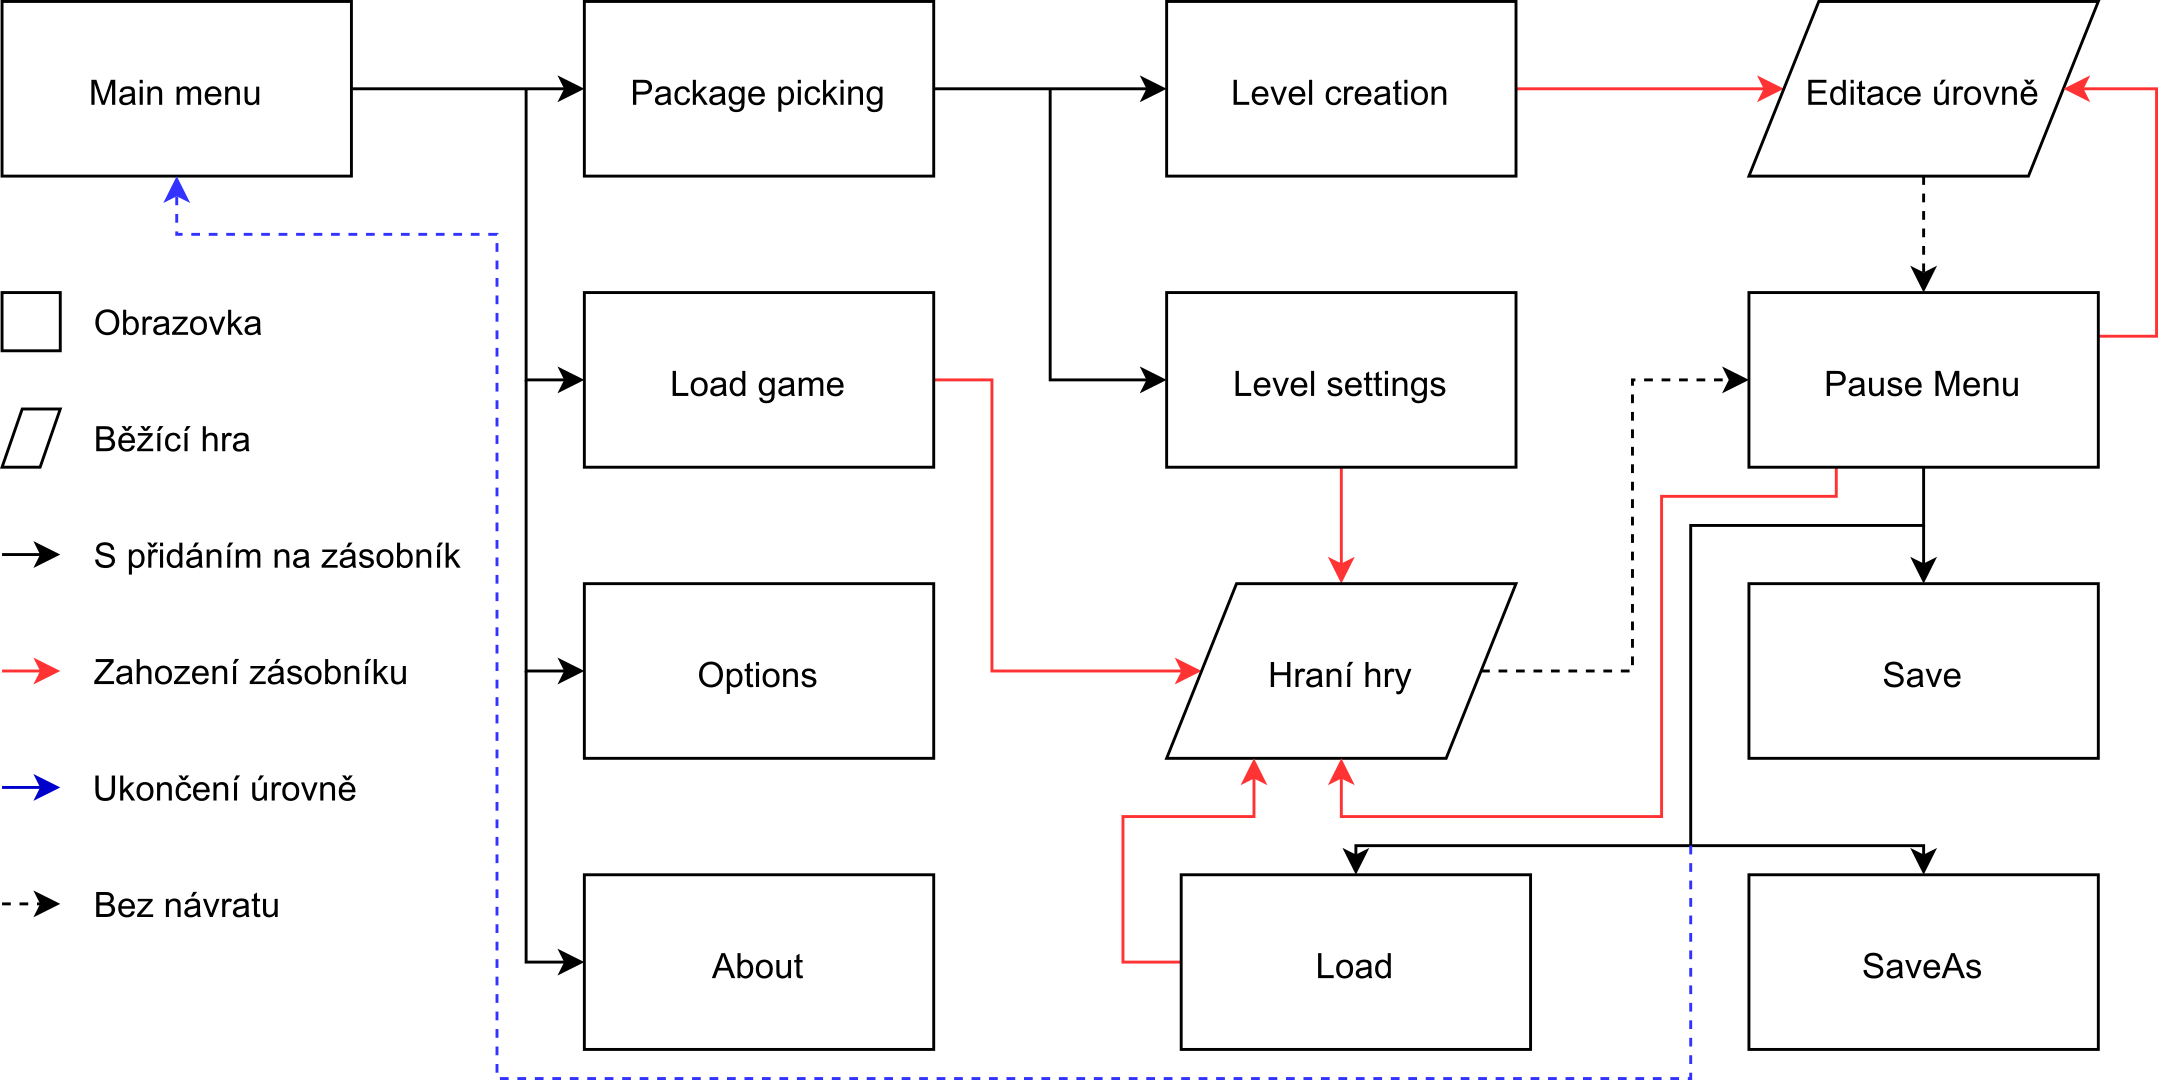
\includegraphics[width=\textwidth]{img/ScreenStructure.png}
	\caption{Obrazovky menu a~přechody mezi nimi.}
	\label{fig:screen_structure2}
\end{figure}

\subsection{Výběr balíčků}
Obrazovka pro výběr balíčků, na diagramu \ref{fig:screen_structure2} označena \texttt{Package picking}, je z~hlavního menu přístupná stisknutím tlačítka \texttt{Start}. Obrazovku můžeme vidět na obrázku \ref{fig:packagepicking}. Centrální část obrazovky zabírá seznam balíčků dostupných v~aktuální instalaci platformy. Každý z~balíčků je reprezentován jednou položkou tohoto seznamu. 

\begin{figure}[h]
	\centering
	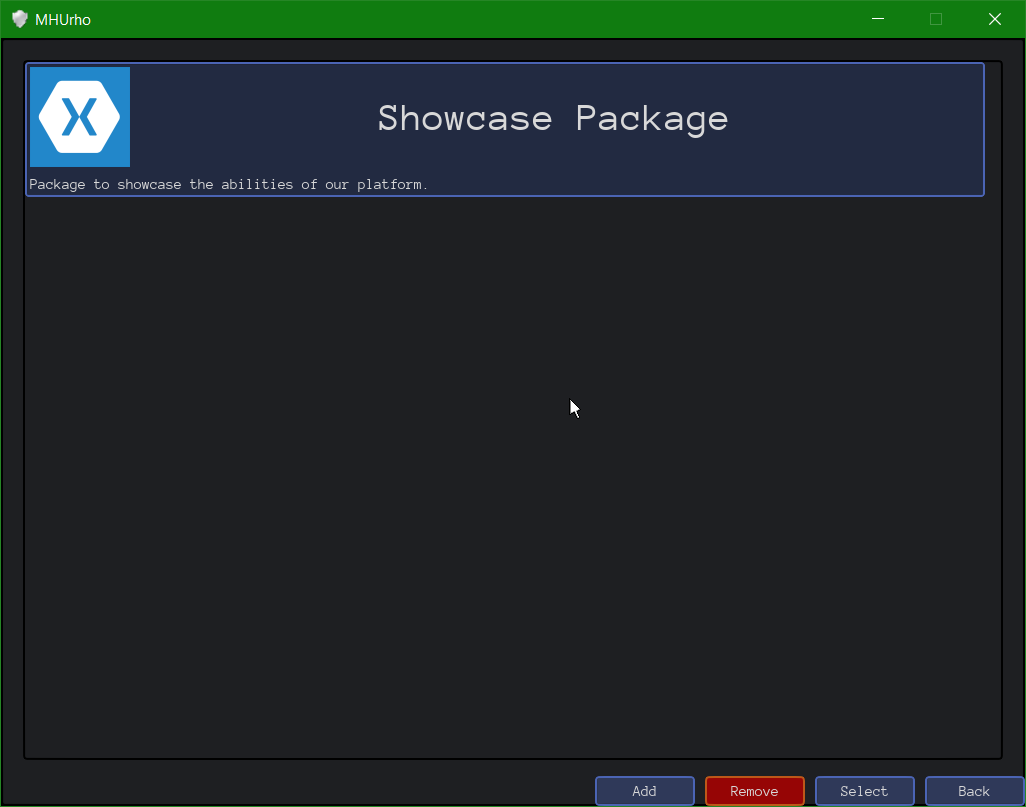
\includegraphics[width=0.5\textwidth]{img/PackagePickingScreen.png}
	\caption{Obrazovky pro výběr balíčku.}
	\label{fig:packagepicking}
\end{figure}

Pro přidání nového balíčků do nainstalované instance platformy přemístěte adresář obsahující soubory balíčku do adresáře \texttt{\%AppData\%/MHUrho/Packages}. Následně stiskněte tlačítko \texttt{Add}, neboli \uv{Přidat}, na obrazovce pro vybírání balíčků. Toto tlačítko vás přesune na obrazovku pro procházení souborového systému. Na této obrazovce poté vyberte XML soubor definující přidávaný balíček. Při návratu na obrazovku pro vybírání balíčků by měl být přidaný balíček viditelný v~seznamu dostupných balíčků. d

Pro smazání balíčku označte položku balíčku v~seznamu a~stiskněte tlačítko \texttt{Remove}. Pro načtení balíčku  označte položku balíčku a~stisknute tlačítko \texttt{Select}. Pro návrat na obrazovku hlavního menu použijte tlačítko \texttt{Back}.

\subsection{Výběr úrovně}
Po vybrání balíčku budete přesunuti na obrazovku výběru úrovně, v~diagramu označenou jako \texttt{Level picking}. Tuto obrazovku můžete vidět na obrázku \ref{fig:levelpicking}. Tato obrazovka poskytuje následující funkce:

\begin{enumerate}
	\item vytváření a~editaci nových úrovní,
	\item editaci existujících úrovní,
	\item spuštění existujících úrovní,
	\item mazání úrovní v~balíčku.
\end{enumerate}

Pro vytvoření nové úrovně označte položku \texttt{Create new level} a~následně stiskněte tlačítko \texttt{Edit}.

\begin{figure}[h]
	\centering
	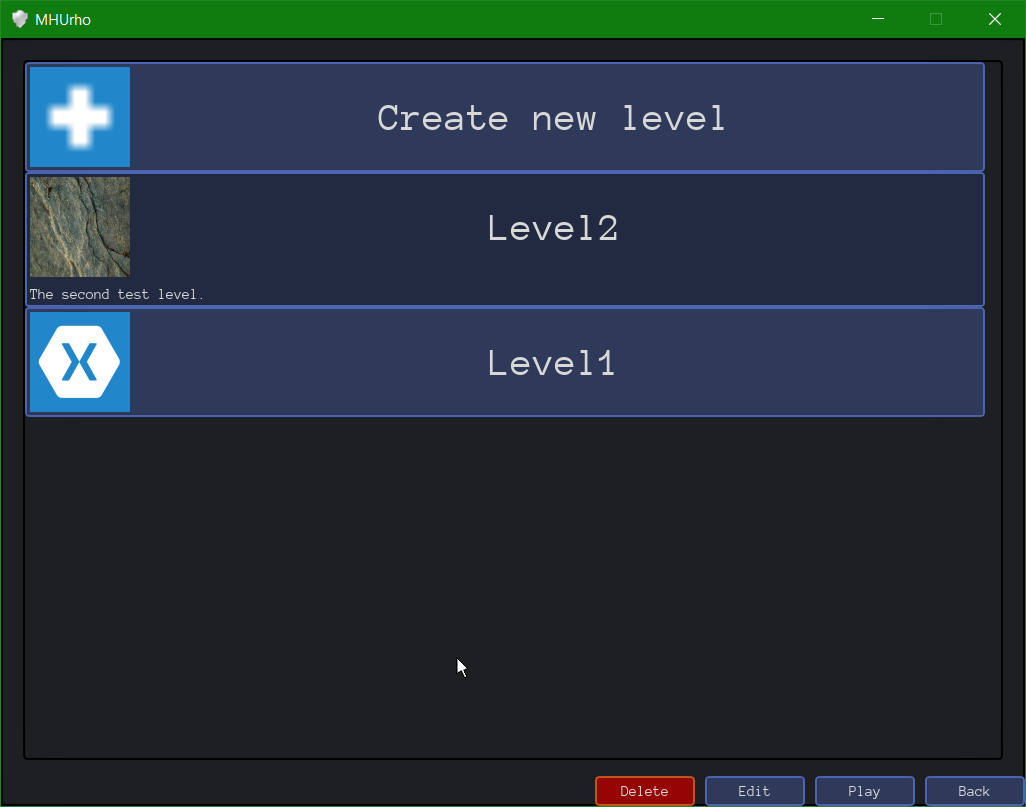
\includegraphics[width=0.5\textwidth]{img/LevelPickingScreen.png}
	\caption{Obrazovky pro výběr úrovně.}
	\label{fig:levelpicking}
\end{figure}

Pro akci s~existující úrovní označte tuto úroveň v~seznamu. Následně stisknutím tlačítka \texttt{Delete} smažete úroveň, stisknutím tlačítka \texttt{Edit} přejdete na obrazovku \texttt{Level creation} a~následně na editaci úrovně a~stisknutím tlačítka \texttt{Play} přejdete na obrazovku \texttt{Level settings} pro nastavení parametrů spuštění úrovně.

Pro návrat na obrazovku výběru balíčků použijte tlačítko \texttt{Back}.
\subsection{Vytváření úrovně}
Při vytváření úrovně či editaci existující úrovně budete přesunuti na obrazovku označenou v~diagramu \ref{fig:screen_structure2} jako \texttt{Level creation}. Vzhled této obrazovky můžete vidět na obrázku \ref{fig:levelcreation}. Jak můžete vidět, tato obrazovka umožňuje nastavit tyto vlastnosti úrovně:

\begin{enumerate}
	\item jméno,
	\item velikost mapy,
	\item plugin logiky,
	\item ikonu,
	\item popis.
\end{enumerate}

Při editaci existující úrovně nelze měnit její velikost a~plugin logiky.

\begin{figure}[h]
	\centering
	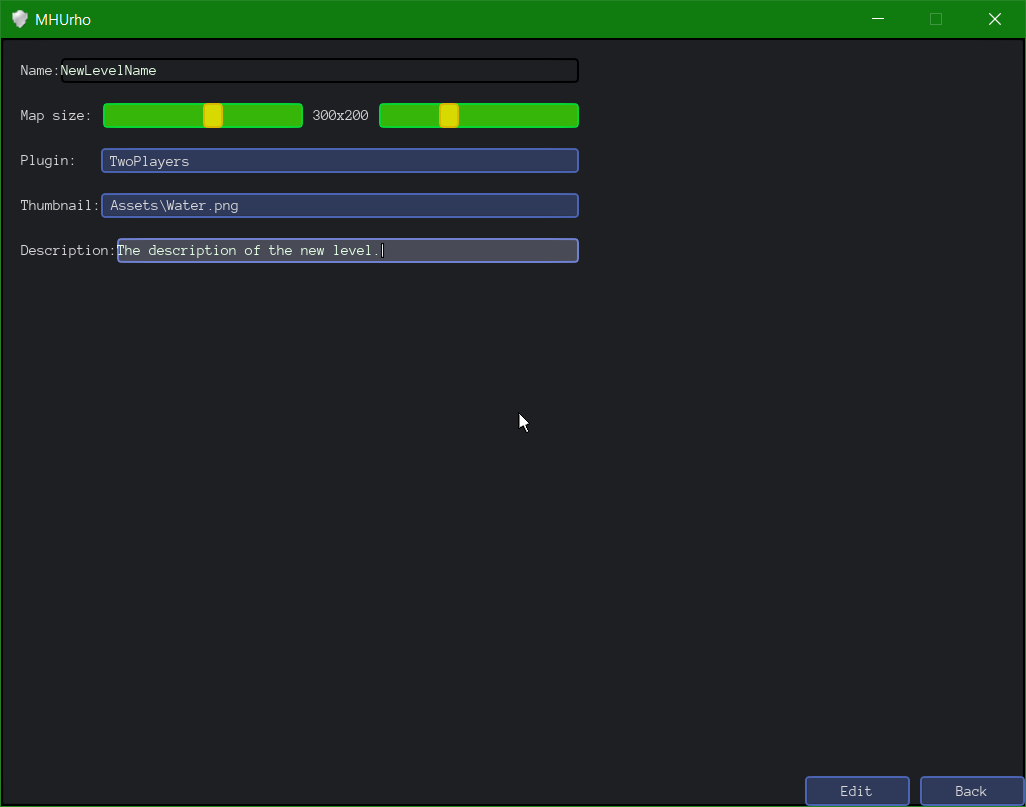
\includegraphics[width=0.5\textwidth]{img/LevelCreationScreen.png}
	\caption{Obrazovky pro nastavení vlastností vytvářené úrovně.}
	\label{fig:levelcreation}
\end{figure}

Pro návrat na obrazovku výběru úrovní použijte tlačítko \texttt{Back}.

\subsection{Nastavení úrovně}
Pro nastavení vlastností úrovně před samotným spuštěním slouží obrazovka \texttt{Level settings}, zobrazená na obrázku \ref{fig:levelsettings}. Obrazovka je rozdělena do čtyř částí:

\begin{enumerate}
	\item výběr pluginu hráčů úrovně a~nastavení jejich příslušenství do týmu;
	\item zobrazení ikony úrovně;
	\item zobrazení prvků grafického uživatelského rozhraní definovaných pluginem úrovně, používaných pro nastavení parametrů spouštěné úrovně;
	\item zobrazení popisu úrovně.
\end{enumerate}

Stisknutím tlačítka \texttt{Play} je spuštěno načítání úrovně a~následně hra. Stisknutím tlačítka \texttt{Back} dojde k~přesunu zpět na obrazovku vybírání úrovní.

\begin{figure}[h]
	\centering
	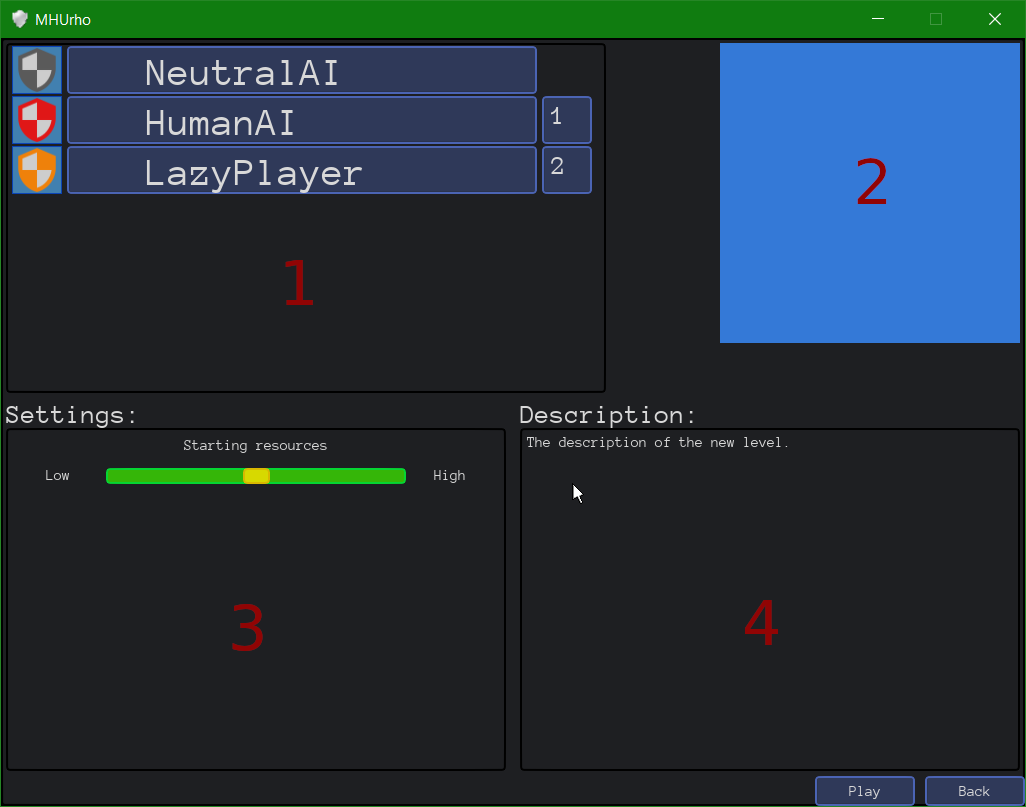
\includegraphics[width=0.5\textwidth]{img/LevelSettingsScreen.png}
	\caption{Obrazovky pro nastavení spuštěné hry.}
	\label{fig:levelsettings}
\end{figure}

\subsection{Přerušení hry}
Při pozastavení hry je zobrazeno tzv.~\texttt{PauseMenu}. Položky tohoto menu se liší podle toho, zda úroveň editujeme či úroveň hrajeme. Porovnání těchto dvou menu můžeme vidět na obrázku \ref{fig:pauseMenu}.

Při editaci umožňuje menu uložit aktuální stav úrovně do balíčkupod jménem nastaveným při vytváření úrovně pomocí tlačítka \texttt{Save} či pod novým jménem pomocí tlačítka \texttt{SaveAs}.

Při hraní hry umožňuje menu uložit aktuální stav hrané hry do adresáře platformy pomocí tlačítka \texttt{Save}, či načíst hranou hru uloženou v~tomto adresáři pomocí tlačítka \texttt{Load}.

\begin{figure}[h]
	\centering
	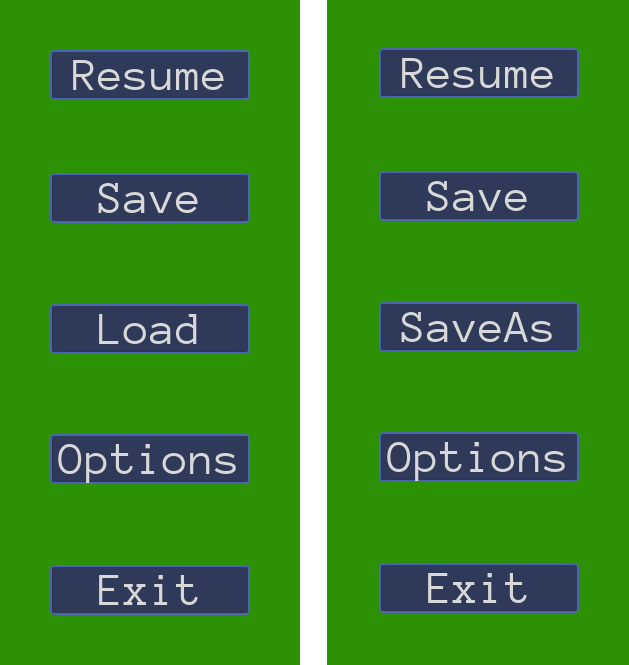
\includegraphics[width=0.5\textwidth]{img/PauseMenuComparison.png}
	\caption{Menu pozastavení hry.}
	\label{fig:pauseMenu}
\end{figure}


\subsection{Výběr souboru}
Obrazovku pro výběr souboru můžeme vidět na obrázku \ref{fig:filepicking}. Modře označená část výpisu obsahu adresáře představuje podadresáře, bílá část pak soubory. V~horní části můžeme vidět vyhledávací řádek, do kterého je možno napsat část jména pro filtrování zobrazených souborů či přímo celou cestu vybíraného souboru či adresáře. Pro výběr lze použít tlačítko \texttt{Select}, které vybere soubor či adresář podle cesty ve vyhledávacím řádku, či dvojklikem na záznam vybíraného souboru.

Obrazovky pro ukládání a~načítání hraných úrovní z~adresáře platformy poskytují navíc tlačítko \texttt{Delete}, kterým je možné uloženou hru smazat.

\begin{figure}[h]
	\centering
	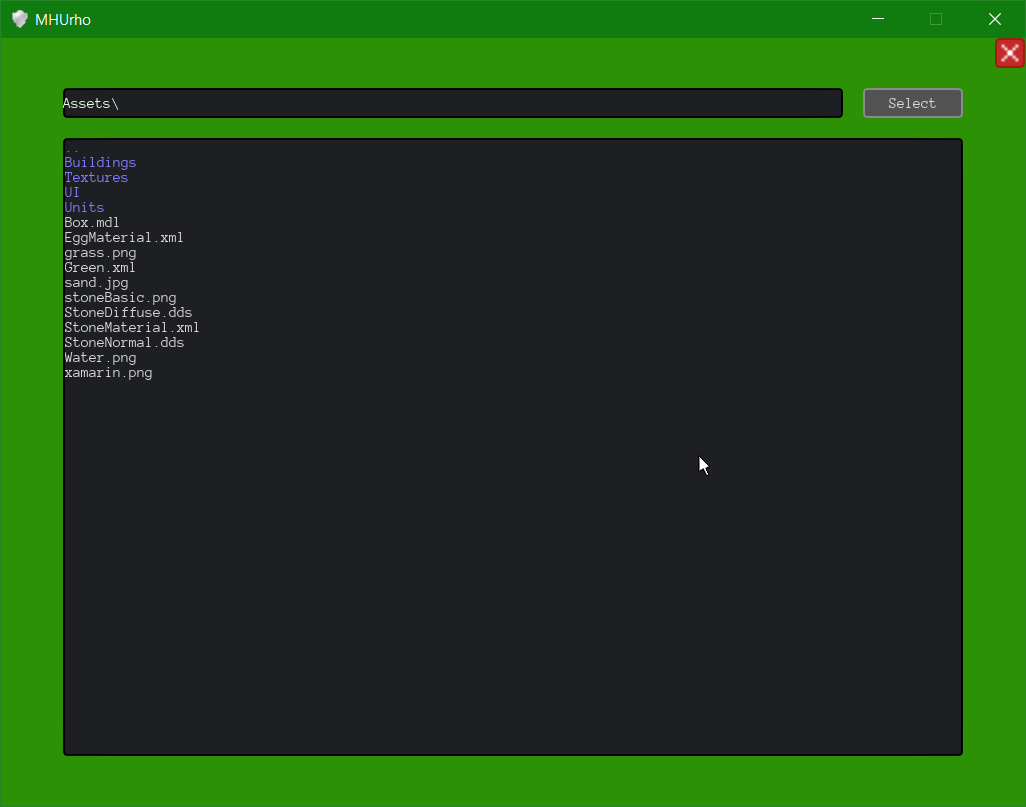
\includegraphics[width=0.5\textwidth]{img/FilePickingScreen.png}
	\caption{Obrazovka pro výběr souboru.}
	\label{fig:filepicking}
\end{figure}

\section{Ukázková hra}
Ukázková hra je reprezentována balíčkem \texttt{ShowcasePackage}. Tento balíček obsahuje jednotky, budovy, projektily a~další součásti hry, které je možné využít pro tvorbu úrovní. Současně obsahuje několik již vytvořených úrovní demonstrujících schopnosti protihráčů, jednotek a~budov.

\subsection{Okno aplikace při hře}
\label{sec:appwindow}
Okno aplikace má při hře platformou definované základní uživatelské rozhraní. Toto rozhraní můžeme vidět na obrázku \ref{fig:UI}. 

Minimapa poskytuje hráči přehled o~stavu velké části mapy bez nutnosti pohybu kamerou. Minimapu lze přibližovat či oddalovat za použití kolečka myši při umístění kurzoru nad minimapu. Dále lze kliknutím přesunout kameru na odpovídající pozici v~herním světě. V~neposlední řadě lze minimapu použít k~rychlému přesunu kamery pomocí kliknutí a~držení levého tlačítka a~posunu myší. Pozice kliknutí se stává středem pomyslného joysticku, který ovládáme posunem myši odpovídajícím směrem.

Centrální lišta obsahuje tlačítka určená aktuálně zvoleným nástrojem. Při velkém počtu tlačítek je možno touto lištou posouvat za použití tlačítek označených šipkami na pravé a~levé straně lišty.

Nad lištou vidíme vpravo tlačítko pro výběr aktuálního hráče a~vlevo tlačítko pro výběr nástroje. Výběr hráče je možný pouze při editaci úrovně. Při hraní je toto tlačítko neaktivní a~pouze zobrazuje ikonu hráče reprezentujícího uživatele. Tlačítko pro výběr budovy, stejně jako tlačítko pro výběr hráče při editaci, při kliknutí zobrazí vysouvací lištu, označenou fialově. Tato lišta obsahuje seznam dostupných nástrojů či seznam dostupných hráčů.

Poslední součástí v~levém dolním rohu je \texttt{CustomWindow}. Obsah této části je určen aktuálním nástrojem. Nejčastěji je v~této části uváděn název nástroje či součásti nástroje, nastavní velikosti štětce, cena budov a~další.

Balíček může do uživatelského rozhraní dodat vlastní prvky, jak můžeme vidět ve vrchní části obrazovky, ve které balíček ukázkové hry umisťuje lištu pro zobrazení množství surovin vlastněných hráčem.

\begin{figure}[h]
	\centering
	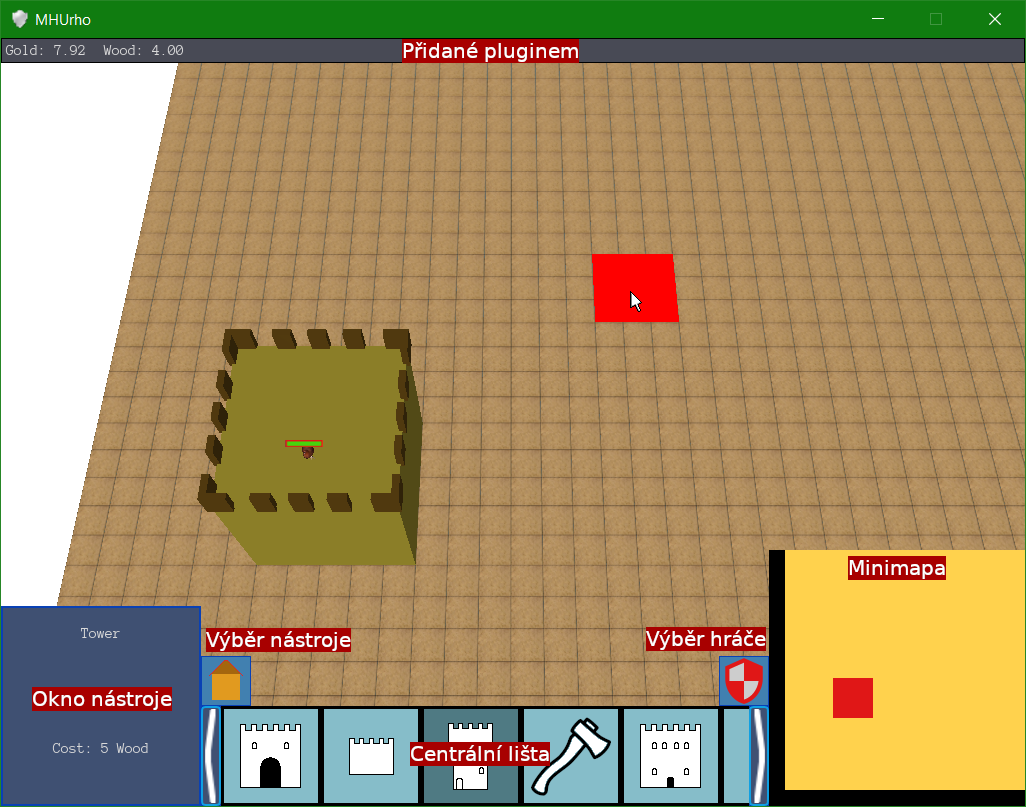
\includegraphics[width=0.5\textwidth]{img/GameUI.png}
	\caption{Uživatelské rozhraní ukázkové hry.}
	\label{fig:UI}
\end{figure}

\subsection{Editor}
Každý z~balíčků, tedy i~ukázková hra, může použít nástroje poskytované platformou či definovat své vlastní nástroje pro editaci úrovně. V~této části popíšeme použití nástrojů dostupných v~editoru úrovní ukázkové hry.

\subsubsection{Nástroje}

Výběr nástroje lze provést stisknutím tlačítka označeného na obrázku \ref{fig:UI} jako \textit{Výběr nástroje}. Stisknutím tohoto tlačítka je zobrazena lišta se seznamem všech dostupných nástrojů, kterou můžete vidět na obrázku \ref{fig:toolselection}. V této liště můžeme vidět označený aktuálně vybraný nástroj, jehož vzhled přebírá také tlačítko pro výběr nástroje. 

Stisknutím tlačítka jiného nástroje než aktuálně vybraného je tento nástroj aktivován a je schována lišta pro výběr nástrojů.

Následuje seznam nástrojů dostupných v ukázkové hře. U každého z nástrojů je uvedeno, ve kterých módech je možné ho využít. Bližší popis jednotlivých nástrojů můžete najít následujících částech.

\medskip
\noindent{
	\begin{minipage}{0.15\textwidth}
		
\includegraphics{TerrainManipulatorTool}
	\end{minipage} \hfill
	\begin{minipage}{0.8\textwidth}
		\textbf{Nástroj pro změnu výšky terénu} umožňuje změnu výšky jednotlivých rohů dlaždic, celých dlaždic uvnitř čtverce či vyhlazení rozdílů ve výšce dlaždic uvnitř čtverce. Tento nástroj je dostupný pouze v editačním módu.
	\end{minipage}	
}

\medskip
\noindent{
	\begin{minipage}{0.15\textwidth}
		
\includegraphics{TileTypeTool}
	\end{minipage} \hfill
	\begin{minipage}{0.8\textwidth}
		\textbf{Nástroj pro změnu typů dlaždic} umožňuje změnu typu dlaždic. Tento nástroj je dostupný pouze v editačním módu.
	\end{minipage}
}

\medskip
\noindent{
	\begin{minipage}{0.15\textwidth}
		
\includegraphics{UnitSelectorTool}
	\end{minipage} \hfill
	\begin{minipage}{0.8\textwidth}
		\textbf{Nástroj pro výběr a ovládání jednotek} umožňuje označit vybrat skupinu jednotek a následně této skupině vydávat rozkazy pro pohyb či pro útok. Tento nástroje je dostupný v editačním i herním módu.
	\end{minipage}
}

\medskip
\noindent{
	\begin{minipage}{0.15\textwidth}
		
\includegraphics{UnitSpawningTool}
	\end{minipage} \hfill
	\begin{minipage}{0.8\textwidth}
		\textbf{Nástroj pro vytváření jednotek} umožňuje přidat do úrovně jednotky vlastněné aktuálně ovládaným hráčem. Tento nástroje je dostupný pouze v editačním módu.
	\end{minipage}
}

\medskip
\noindent{
	\begin{minipage}{0.15\textwidth}
		
\includegraphics{BuildingBuilderTool}
	\end{minipage} \hfill
	\begin{minipage}{0.8\textwidth}
		\textbf{Nástroj pro stavbu budov} umožňuje přidat do úrovně budovy vlastněné aktuálně ovládaným hráčem. Tento nástroje je dostupný v editačním i herním módu.
	\end{minipage}
}

\subsubsection{Nástroj pro změnu výšky terénu}
Tento nástroj umožňuje měnit reliéf terénu aktuální úrovně. Nástroj je složen ze čtyř součástí. Těmito součástmi jsou:

\medskip
\noindent{
	\begin{minipage}{0.15\textwidth}
		
\includegraphics{VertexSelection}
	\end{minipage} \hfill
	\begin{minipage}{0.8\textwidth}
		Výběr rohů dlaždic.
	\end{minipage}
}

\medskip
\noindent{
	\begin{minipage}{0.15\textwidth}
		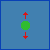
\includegraphics{VertexMovement}
	\end{minipage} \hfill
	\begin{minipage}{0.8\textwidth}
		Změny výšky vybraných rohů dlaždic.
	\end{minipage}
}

\medskip
\noindent{
	\begin{minipage}{0.15\textwidth}
		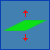
\includegraphics{TileMovement}
	\end{minipage} \hfill
	\begin{minipage}{0.8\textwidth}
		Změna výšky dlaždic uvnitř zvýrazněného čtverce.
	\end{minipage}
}

\medskip
\noindent{
	\begin{minipage}{0.15\textwidth}
		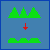
\includegraphics{Smoothing}
	\end{minipage} \hfill
	\begin{minipage}{0.8\textwidth}
		Vyhlazen rozdílů výšky dlaždic uvnitř zvýrazněného čtverce.
	\end{minipage}
}
\bigskip


První dvě součásti jsou dohromady používány pro výběr jednotlivých rohů dlaždic v mapě a následnou úpravu jejich výšky. Výběr lze provést zvolením části pro výběr rohů a následným kliknutím na dlaždici obsahující daný roh. Je vybrán roh nejbližší pozici kliknutí. Zrušení výběru lze následně provést pokusem o výběr již vybraného rohu. Pro změnu výšky vybraných rohů zvolíme část pro změnu výšky vybraných rohů. Po jejím zvolení můžeme kliknutím a držením levého tlačítka a posouváním myši nahoru a dolu měnit výšku vybraných rohů.

Součást pro změnu výšky dlaždic umožňuje pohybem kurzoru po herním světě vybrat čtverec dlaždic okolo pozice kurzoru, jejichž výšku měníme pomocí stisknutí a držení levého tlačítka a pohybem myši stejně jako u předchozí části.

Poslední součást pro vyhlazení terénu umožňuje stisknutím a držením levého tlačítka myši a pohybem po mapě vyrovnávat rozdíly výšky terénu.

\subsubsection{Nástroj pro změnu typu dlaždic}
Při zvolení tohoto nástroje je centrální lišta vyplněna všemi dostupnými typy dlaždic v balíčku. V ukázkovém balíčku bude centrální lišta vyplněna těmito ikonami:

\medskip
\noindent{
	\begin{minipage}{0.1\textwidth}
		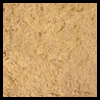
\includegraphics[scale=0.3]{SandIcon}
	\end{minipage} \hfill
	\begin{minipage}{0.85\textwidth}
		Ikona typu dlaždic \texttt{Sand}, neboli písek.
	\end{minipage}
}

\medskip
\noindent{
	\begin{minipage}{0.1\textwidth}
		
\includegraphics[scale=0.3]{XamarinIcon}
	\end{minipage} \hfill
	\begin{minipage}{0.85\textwidth}
		Ikona typu dlaždic \texttt{Xamarin}.
	\end{minipage}
}

\medskip
\noindent{
	\begin{minipage}{0.1\textwidth}
		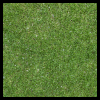
\includegraphics[scale=0.3]{GrassIcon}
	\end{minipage} \hfill
	\begin{minipage}{0.85\textwidth}
		Ikona typu dlaždic \texttt{Grass}, neboli tráva.
	\end{minipage}
}

\medskip
\noindent{
	\begin{minipage}{0.1\textwidth}
		
\includegraphics[scale=0.3]{WaterIcon}
	\end{minipage} \hfill
	\begin{minipage}{0.85\textwidth}
		Ikona typu dlaždic \texttt{Water}, neboli voda.
	\end{minipage}
}

\medskip
\noindent{
	\begin{minipage}{0.1\textwidth}
		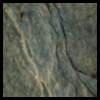
\includegraphics[scale=0.3]{StoneIcon}
	\end{minipage} \hfill
	\begin{minipage}{0.85\textwidth}
		Ikona typu dlaždic \texttt{Stone}, neboli kámen.
	\end{minipage}
}

\bigskip

Vybráním typu dlaždic z tohoto seznamu, umístěním kurzoru do herního světa a stisknutím levého tlačítka změníme typ dlaždic zvýrazněného čtverce na zvolený typ.

Pokud podržíme levé tlačítko a budeme pohybovat myší, budou změněny všechny dlaždice kterých se dotkně zvýrazněná část.

Velikost zvýrazněné části lze nastavit v okně nástrojů pomocí grafického prvku přidaného tímto nástrojem.

\subsubsection{Nástroj pro výběr a ovládání jednotek}
Tento nástroj umožňuje vybrat skupinu jednotek aktuálního hráče. Tento výběr uskutečníme stisknutím a držením levého tlačítka a následným tažením myši po herním světě. Mezi počáteční pozicí stisku a aktuální pozicí kurzoru se vytvoří obdélník označující oblast, ve které budou jednotky vybrány. Po uvolnění tlačítka myši budou všechny jednotky vlastněné aktuálním hráčem přidány do aktuálně vybrané skupiny jednotek. Jednotky lze označovat i jednotlivě kliknutím na jednotku vlastněnou aktuálním hráčem.

Následně lze vybraným jednotkám vydávat rozkazy. Kliknutím levým tlačítkem vydáme rozkaz k pohybu na aktuální pozici kurzoru. Kliknutím pravím tlačítkem na nepřátelskou jednotku či budovu pak vydáme rozkaz k útoku na tuto jednotku či budovu.

\subsubsection{Nástroj pro vytváření jednotek}
Tento nástroj umožňuje přidávat do aktuální úrovně nové jednotky či odebírat existující. Po zvolení tohoto nástroje je centrální lišta naplněna ikonami všech dostupných jednotek, které je možné manuálně přidávat do úrovně. Nejvíce vpravo je pak přidána ikona umožňující mazání existujících jednotek. V ukázkovém balíčku tedy bude centrální lišta vyplněna následujícími ikonami:

\medskip
\noindent{
	\begin{minipage}{0.1\textwidth}
		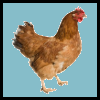
\includegraphics[scale=0.3]{ChickenIcon}
	\end{minipage} \hfill
	\begin{minipage}{0.85\textwidth}
		Ikona typu jednotek \texttt{Chicken}.
	\end{minipage}
}

\medskip
\noindent{
	\begin{minipage}{0.1\textwidth}
		
\includegraphics[scale=0.3]{WolfIcon}
	\end{minipage} \hfill
	\begin{minipage}{0.85\textwidth}
		Ikona typu jednotek \texttt{Wolf}.
	\end{minipage}
}

\medskip
\noindent{
	\begin{minipage}{0.1\textwidth}
		
\includegraphics[scale=0.3]{Deleter}
	\end{minipage} \hfill
	\begin{minipage}{0.85\textwidth}
		Ikona pro odstraňování jednotek.
	\end{minipage}
}


\bigskip


Pro vytvoření nové jednotky vybereme jeden z poskytovaných typů a následným kliknutím do herního světa vytvoříme na pozici kurzoru novou jednotku vybraného typu.

Pro odstranění jednotky vybereme ikonu pro odstraňování jednotek. Následným kliknutím na jednotku tuto jednotku odstraníme z úrovně.

Funkcionalita tohoto nástroje je při hraní úrovně nahrazena budovou tvrze, popsanou v~části \ref{sec:buildings}.


\subsubsection{Nástroj pro stavbu budov}
\label{sec:buildingbuilder}
Tento nástroj umožňuje v editačním i v herním módu přidávat do herního světa budovy vlastněné aktuálně ovládaným hráčem. Při zvolení tohoto nástroje je centrální lišta vyplněna ikonami všech budov dostupných v balíčku. V ukázkovém balíčku bude centrální lišta vyplněna těmito ikonami:

\medskip
\noindent{
	\begin{minipage}{0.1\textwidth}
		
\includegraphics[scale=0.3]{KeepIcon}
	\end{minipage} \hfill
	\begin{minipage}{0.85\textwidth}
		Ikona typu budov \texttt{Keep}.
	\end{minipage}
}

\medskip
\noindent{
	\begin{minipage}{0.1\textwidth}
		
\includegraphics[scale=0.3]{GateIcon}
	\end{minipage} \hfill
	\begin{minipage}{0.85\textwidth}
		Ikona typu budov \texttt{Gate}.
	\end{minipage}
}

\medskip
\noindent{
	\begin{minipage}{0.1\textwidth}
		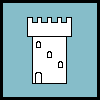
\includegraphics[scale=0.3]{TowerIcon}
	\end{minipage} \hfill
	\begin{minipage}{0.85\textwidth}
		Ikona typu budov \texttt{Tower}.
	\end{minipage}
}

\medskip
\noindent{
	\begin{minipage}{0.1\textwidth}
		
\includegraphics[scale=0.3]{WallIcon}
	\end{minipage} \hfill
	\begin{minipage}{0.85\textwidth}
		Ikona typu budov \texttt{Wall}.
	\end{minipage}
}

\medskip
\noindent{
	\begin{minipage}{0.1\textwidth}
		
\includegraphics[scale=0.3]{TreeCutterIcon}
	\end{minipage} \hfill
	\begin{minipage}{0.85\textwidth}
		Ikona typu budov \texttt{TreeCutter}.
	\end{minipage}
}

\medskip
\noindent{
	\begin{minipage}{0.1\textwidth}
		
\includegraphics[scale=0.3]{TreeIcon}
	\end{minipage} \hfill
	\begin{minipage}{0.85\textwidth}
		Ikona typu budov \texttt{Tree}.
	\end{minipage}
}

\medskip
\noindent{
	\begin{minipage}{0.1\textwidth}
		
\includegraphics[scale=0.3]{Deleter}
	\end{minipage} \hfill
	\begin{minipage}{0.85\textwidth}
		Ikona pro odstraňování budov.
	\end{minipage}
}

\bigskip

Následně vybráním jedné z těchto budov a kliknutím na dlaždici je do herního světa umístěna nová budova se středem na dané dlaždici. Tento nástroj dále umožňuje ovládání a mazání existujících budov. 

Ovládání je umožněno při aktivaci nástroje bez vybrané budovy, což následně umožňuje kliknutím na budovu zobrazit rozhraní pro její ovládání.

Mazání je umožněno výběrem ikony červeného čtverce a následným kliknutím na existující budovu.

\subsection{Ovládání kamery}
Kamera je schopna pohybu v~několika módech. Těmito módy jsou RTS mód, \texttt{FreeFloat} mód a~sledování jednotky. Přepínání mezi RTS a \texttt{FreeFloat} módem je prováděno klávesou \textit{Shift}. Přepnutí na sledování jednotky je možné kliknutím pravého tlačítka na jednotku. Následná lze přejít zpět na RTS mód pokusem o~pohnutí kamerou, či na \texttt{FreeFloat} mód pomocí klávesy \textit{Shift}.

Pohyb v~módech RTS a \texttt{FreeFloat} lze ovládat pomocí klávesnice. Klávesy \textit{W}, \textit{S}, \textit{A}, \textit{D} umožňují pohyb kamery vpřed, vzad, vlevo a~vpravo. 

V~módu RTS lze také ovládat pohyb kamery pomocí umístění myší na okraj obrazovky, načež se kamera začne posouvat směrem k~tomuto okraji. 

Otáčení kamery lze v~RTS módu a~módu sledování jednotky provést klávesami \textit{Q} a \texttt{E} pro otáčení vlevo či vpravo, a~klávesami \textit{R} a \textit{F} pro otáčení vzhůru a~dolu. 

V~módu \texttt{FreeFloat} lze otáčet kamerou pouze pomocí myši.   

\subsection{Budovy}
\label{sec:buildings}
Ukázkový balíček obsahuje šest typů budov. První čtyři typy označujeme jako obranné budovy, sloužící především pro zamezení průchodu nepřátelských jednotek a~umožňující zvýšení dostřelu vlastních jednotek pomocí umístění jednotek na tyto budovy. Mezi tyto budovy patří \texttt{Keep}, neboli tvrz, \texttt{Gate}, neboli brána, \texttt{Tower}, neboli věž a \texttt{Wall}, neboli hradba. Zbylé dva typy slouží pro získávání dřeva. Těmito budovami jsou \texttt{Tree}, neboli strom, a \texttt{TreeCutter}, neboli dřevorubec. 

\medskip
\noindent{
	\begin{minipage}{0.15\textwidth}
		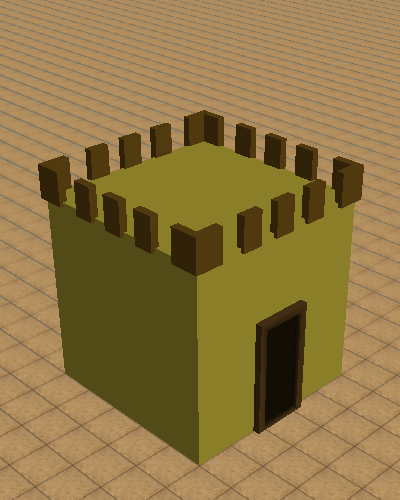
\includegraphics[scale=0.6]{Keep}
	\end{minipage} \hfill
	\begin{minipage}{0.8\textwidth}
		\textbf{Keep}, neboli tvrz. Každý hráč vlastní právě jednu tuto budovu, při jejímž zničení hráč prohrává. Cílem hry je tedy zničit protivníkovu tvrz bez ztráty své vlastní tvrze. Tvrz umožňuje pohyb jednotek po své střeše. Tvrz dále slouží pro tvorbu jednotek během hry. Tato funkce je zpřístupněna pomocí nástroje pro stavbu budov, popsaného v části \ref{sec:buildingbuilder}.
	\end{minipage}
}

\medskip
\noindent{
	\begin{minipage}{0.15\textwidth}
		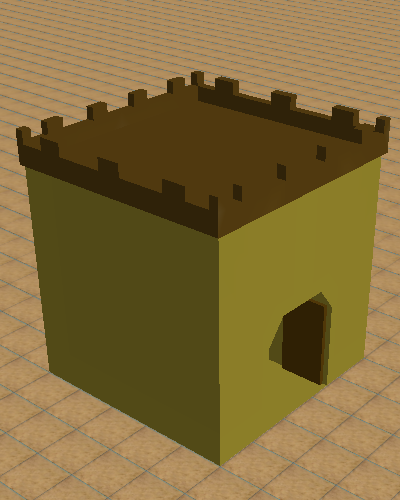
\includegraphics[scale=0.6]{Gate}
	\end{minipage} \hfill
	\begin{minipage}{0.8\textwidth}
		\textbf{Gate}, neboli brána. Brána umožňuje pohyb jednotek jak po své střeše, tak skrz tunel uvnitř této budovy. Střecha této budovy je automaticky propojena se střechami bran, věží a hradeb na přímo sousedících dlaždicích. Dále umožňuje již podle svého názvu zavřít jeden konec tunelu a~tím znemožnit přístup do tunelu z~této strany. Ovládání brány je zpřístupněno pomocí nástroje pro stavbu budov, popsaného v části \ref{sec:buildingbuilder}.
	\end{minipage}
}

\medskip
\noindent{
	\begin{minipage}{0.15\textwidth}
		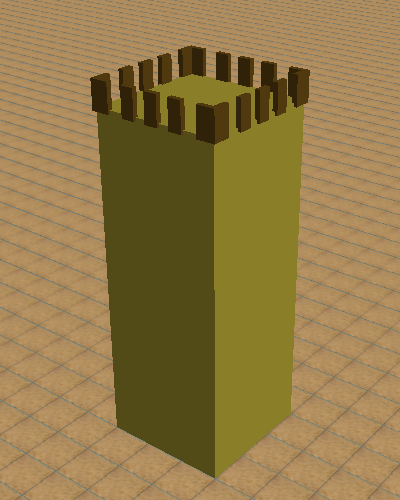
\includegraphics[scale=0.6]{Tower}
	\end{minipage} \hfill
	\begin{minipage}{0.8\textwidth}
		\textbf{Tower}, neboli věž. Tato budova umožňuje chůzi po své střeše a~díky své výšce zvyšuje dostřel jednotek. Její střecha je propojena se střechami bran, věží a hradeb na přímo sousedících dlaždicích.
	\end{minipage}
}

\medskip
\noindent{
	\begin{minipage}{0.15\textwidth}
		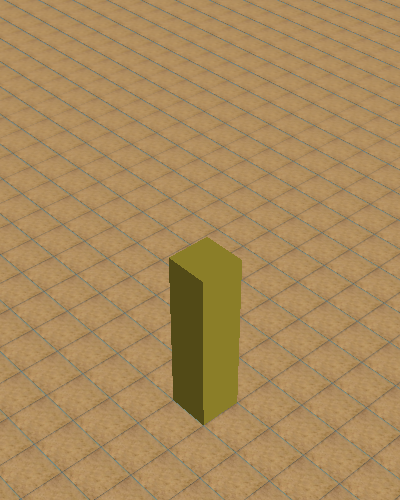
\includegraphics[scale=0.6]{Wall}
	\end{minipage} \hfill
	\begin{minipage}{0.8\textwidth}
		\textbf{Wall}, neboli hradba. Hlavním účelem této budovy je zablokování přístupu do hradu. Dále umožňuje chůzi po své střeše. Střecha je automaticky propojena se střechami bran, věží a hradeb přímo sousedících s touto budovou.
	\end{minipage}
}

\medskip
\noindent{
	\begin{minipage}{0.15\textwidth}
		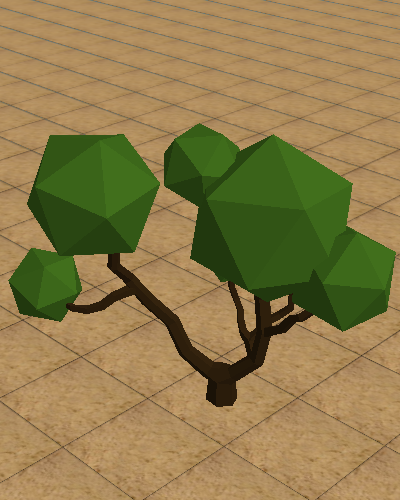
\includegraphics[scale=0.6]{Tree}
	\end{minipage} \hfill
	\begin{minipage}{0.8\textwidth}
		\textbf{Tree}, neboli strom. Stavba stromů je omezena na editaci úrovně a~jejich vlastníkem může být pouze neutrální hráč, tedy hráč s~šedým štítem. Tento hráč jako jediný nemusí vlastnit tvrz, nelze ho zabít a~neútočí na ostatní hráče. Stromy podle typu dlaždice, na které se nacházejí, rostou různou rychlostí a~množí se s~různou pravděpodobností.
	\end{minipage}
}

\medskip
\noindent{
	\begin{minipage}{0.15\textwidth}
		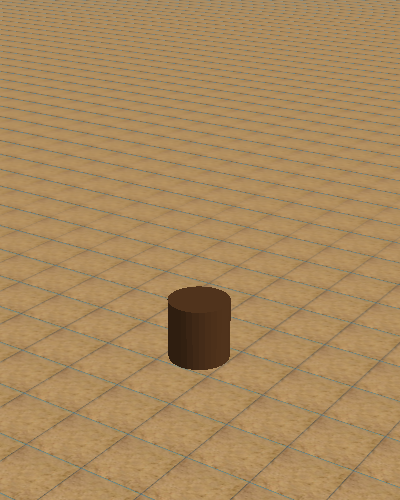
\includegraphics[scale=0.6]{TreeCutter}
	\end{minipage} \hfill
	\begin{minipage}{0.8\textwidth}
		\texttt{TreeCutter}, neboli dřevorubec umožňuje hráči získávat ze stromů dřevo. Tato budova vytváří dvě jednotky, které následně pendlují mezi nejbližším stromem a~touto budovou, čímž získávají pro hráče dřevo.
	\end{minipage}
}

\subsection{Jednotky}
Balíček ukázkové hry definuje tři typy jednotek, z toho dvě ovladatelné hráčem a jednu plně automatickou.

\medskip
\noindent{
	\begin{minipage}{0.15\textwidth}
		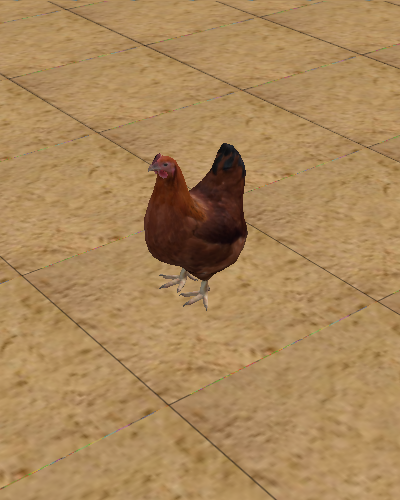
\includegraphics[scale=0.6]{Chicken}
	\end{minipage} \hfill
	\begin{minipage}{0.8\textwidth}
		\textbf{Chicken} je jednotka útočící na dálku, používající vajíčka jako projektily. Dostřel této jednotky závisí na rozdílu její výšky od cíle, je tedy výhodné ji umisťovat na vyvýšená místa, jako například budovy. Oproti vlkům dokáže tento typ jednotek chodit přes vodu a~poškodit obranné budovy.
	\end{minipage}
}

\medskip
\noindent{
	\begin{minipage}{0.15\textwidth}
		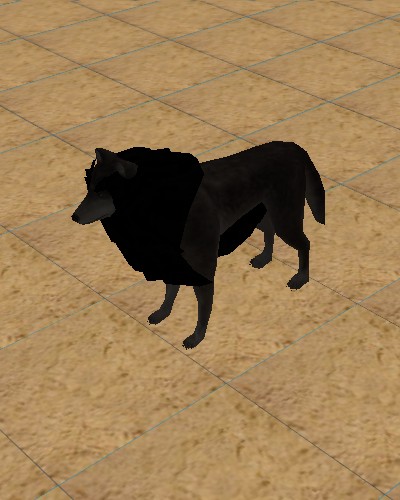
\includegraphics[scale=0.6]{Wolf}
	\end{minipage} \hfill
	\begin{minipage}{0.8\textwidth}
		\textbf{Wolf}, neboli vlk, je jednotka útočící na blízko. Tato jednotka se pohybuje rychleji než \texttt{Chicken} nebo \texttt{Dog}. Tato jednotka nedokáže poškodit nepřátelské obranné budovy.
	\end{minipage}
}

\medskip
\noindent{
	\begin{minipage}{0.15\textwidth}
		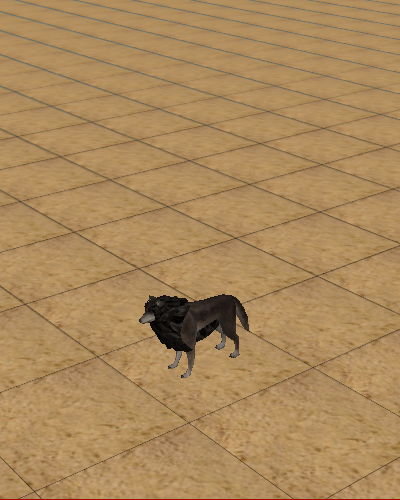
\includegraphics[scale=0.6]{Dog}
	\end{minipage} \hfill
	\begin{minipage}{0.8\textwidth}
		\textbf{Dog}, neboli pes, je jednotka vytvářená budovou dřevorubce, která se pohybuje mezi budovou a nejbližším stromem a získává tak dřevo. Tuto jednotku nelze manuálně vytvářet ani ovládat, vše je plně automatizováno. 
	\end{minipage}
}

\subsection{Projektily}
Ukázková hra definuje pouze jeden projektilů, ze kterých je pouze jeden aktuálně využíván. Těmito typy jsou:

\begin{enumerate}
	\item \texttt{EggProjectile},
	\item \texttt{TestProjectile}.
\end{enumerate}

První typ je využíván jednotkou \texttt{Chicken}. Tento typ má jednoduchou logiku využívající komponenty \texttt{BallisticProjectile} pro implementaci svého pohybu. Drhý typ ukazuje možnosti složitějšího chování projektilu. Tento projektil také využívá pro implementaci svého pohybu komponentu \texttt{BallisticProjectile}, ale dále přidává dodatečné chování. Po určité době od výstřelu se tento projektil rozdělí na více projektilů stejného druhu, čímž vytvoří efekt brokovnice a~pokryje projektily okolí svého původního dopadu. Dále tento projektil ukazuje zpožděné odstranění z~úrovně, díky kterému zůstává určitou chvíli zaseknutý v~terénu.

\subsection{Umělé inteligence hráčů}
Ukázková hra poskytuje dvě umělé inteligence nepřátelských hráčů, kterými jsou:

\begin{enumerate}
	\item \texttt{LazyPlayer},
	\item \texttt{AggressivePlayer}.
\end{enumerate}

Lazy player je jednoduchá umělá inteligence, která nic nedělá. Jejím hlavním účelem umožnění uživately vyzkoušení herního režimu platformy a~možnost stavby svého hradu bez jakéhokoli ohrožení nepřítelem.

AggressivePlayer je aktivní umělá inteligence, která staví budovy pro získávání dřeva, jednotky pro obranu svého tvrze a~útok na nejbližšího nepřátelského hráče.

\subsection{Umělé inteligence úrovní}
Ukázková hra je příkladem balíčku, který všechnu svou logiku decentralizuje do jednotek, budov, projektilů a~hráčů. Z~tohoto důvodu obsahují dvě logiky definované ukázkovou hrou minimum herní logiky. Ukázková hra poskytuje tyto dvě logiky:

\begin{enumerate}
	\item \texttt{TwoPlayerLogic},
	\item \texttt{FourPlayerLogic}.
\end{enumerate}

Obě tyto logiky poskytují požadované metody informace platformě ve formě \texttt{ToolManageru} a \texttt{AStarFactory}. 

První logika již podle názvu definuje úrovně se dvěma hráči. Dále poskytuje možnost před prvním spuštěním úrovně nastavit počáteční množství surovin vlastněné hráči.
Druhá logiky definuje úrovně se čtyřmi hráči a~určuje pevné množství počátečních surovin.


\chapter*{Závěr}
\addcontentsline{toc}{chapter}{Závěr}
Na závěr práce shrneme implementaci naší platformy a porovnáme ji s našimi cíli, uvedenými v části \ref{sec:cileprace}.

Výsledkem naší práce je platformu pro tvorbu 3D RTS her pro jednoho hráče, implementovaná pomocí jazyka C\# a enginu UrhoSharp. Tato platforma umožňuje tvorbu balíčků, které lze distribuovat separátně od platformy a přidávat i do nainstalované instance platformy. Tyto balíčky mohou obsahovat nové typy jednotek, budov, projektilů, nepřátelských hráčů, nástrojů pro editaci map a dalších herních prvků, které je možné využít pro tvorbu a hraní map. 

Platforma umožňuje tvorbu jednotek schopných pohybu po herním světě, řízeného jak rozkazy hráče, tak umělou inteligencí jednotek. Jednotky je možné vytvářet během editace úrovně i v průběhu hry. Jednotky jsou schopné útočit na dálku, na blízko či oběma způsoby najednou na rozkaz hráče či z rozhodnutí umělé inteligence. Při zásahu je jednotka o této události informována, což umožňuje implementaci systému \textit{hit-pointů}.

Budovy lze v platformě umisťovat do herního světa jak při editaci mapy, tak v průběhu hry. Následně je možné v průběhu hry budovy poškozovat a při dostatečném poškození následně zničit. Dále dokáží budovy rozšiřovat prostor dostupný jednotkám mimo úroveň terénu. V neposlední řadě platforma umožňuje vytvářet budovy produkují suroviny, vytvářející jednotky či stavějící další budovy.

Z pohledu surovin platforma umožňuje přidávání a odebírání libovolného množství surovin způsobeného akcí hráče, jednotky, budovy či uplynutím času, čímž je umožněna implementace aktivního i pasivního získávání surovin.

Dostupnost jednotek a budov pro tvorbu hráčem je plně v rukou tvůrce pluginů, čímž platforma umožňuje implementaci systémů technologií a postupného odemykání typů jednotek a budov.

Implementace mapy je v platformě rozdělena na čtvercové dlaždice, umožňující změnu výšek svých jednotlivých rohů. Každé dlaždici je přiřazen typ, který je spolu s přítomnými jednotkami a budovami na dlaždici možné využít pro rozhodování v implementaci pluginů.

Systém balíčků umožňuje vytvářet balíčky obsahující typy těchto herních prvků:
\begin{enumerate}
	\item jednotek,
	\item budov,
	\item projektilů,
	\item surovin,
	\item dlaždic,
	\item hráčů,
	\item úrovní.	
\end{enumerate} 
Pro typy s grafickou reprezentací v herním světě umožňuje balíček přidání modelů a textur. Pro typy, které umožňují autonomní chování, je umožněno přidat pluginy, které následně toto chování definují.

Z pohledu koncového uživatele platforma poskytuje grafické rozhraní pro stolní počítače, umožňuje přidávání a výběr balíčků a následný výběr či tvorbu úrovní z těchto balíčků. Dále platforma poskytuje ukládání a načítání aktuálního stavu hry.

Ukázková hra následně demonstruje výše popsané vlastnosti pomocí několika typů jednotek, budov, surovin, projektilů, hráčů a úrovní.


Z popisu platformy tedy můžeme uznat cíle práce, uvedené v části \ref{sec:cileprace}, za splněné.

\section{Možná rozšíření}
Přestože je aktuální verze platformy plně funkční a splňuje všechny cíle naší práce, existuje několik oblastí, v kterých by mohla být platforma rozšířena:

\begin{itemize}
	\item Implementace podpory pro systém Android, jejíž kostra je v aktuální verzi připravena.
	\item Přidání dalších typů jednotek a budov, poskytujících větší strategické možnosti při hraní ukázkové hry. Aktuální budovy a jednotky v ukázkové hře slouží pouze pro demonstraci schopností platformy a nejsou navrženy s ohledem na jejich použití hráčem.
	\item Množina umělých inteligencí hráčů je v aktuální verzi omezena pouze na dvě možnosti, a to hráče, který nedělá nic, a hráče, který je agresivní a útočí. V budoucnu by bylo výhodné přidat hráče, kteří i brání, či vytvářejí svoji strategii pomocí složitějších postupů.
	\item Verze platformy distribuovaná s touto prací obsahuje pouze jeden balíček, obsahující ukázkovou hru. Pro budoucí verze platformy by bylo užitečné přidat další balíčky, poskytující jiné typy her.
	\item Vylepšení návrhu a vzhledu uživatelského rozhraní platformy i hry. Aktuální uživatelské rozhraní je navrženo především pro demonstraci schopností platformy a nedbá příliš na estetiku či jednoduchost používání. 
	\item Přidání tzv.~\uv{Fog of War} funkcionality, která zakrývá části mapy vzdálené od jednotek a budov hráče a jeho spojenců. Tato funkcionalita je přítomná ve velké části RTS her a její přítomnost by rozšířila množinu her implementovatelných v naší platformě.
	\item I když cílem naší práce byla tvorba platformy pro hry jednoho hráče, použitý herní engine podporuje tvorbu her pro více hráčů. Využitím těchto služeb by mělo být možné přidat mód pro více hráčů.
	\item Platforma umožňuje tvůrcům pluginů implementovat vlastní algoritmy pro hledání nejkratší cesty v herním světě. V aktuální verzi navíc platforma poskytuje jednu implementaci algoritmu A* pro tento účel. V budoucnu by mohlo být výhodné přidat další algoritmy přímo do platformy a poskytnout je tak tvůrcům pluginů.
	
\end{itemize}


%%% Seznam použité literatury
%%% Seznam použité literatury (bibliografie)
%%%
%%% Pro vytváření bibliografie používáme bibTeX. Ten zpracovává
%%% citace v textu (např. makro \cite{...}) a vyhledává k nim literaturu
%%% v souboru literatura.bib.
%%%
%%% Příkaz \bibliographystyle určuje, jakým stylem budou citovány odkazy
%%% v textu. V závorce je název zvoleného souboru .bst. Styly plainnat
%%% a unsrt jsou standardní součástí latexových distribucí. Styl czplainnat
%%% je dodáván s touto šablonou a bibTeX ho hledá v aktuálním adresáři.

\bibliographystyle{czplainnat}    %% Autor (rok) s českými spojkami
% \bibliographystyle{plainnat}    %% Autor (rok) s anglickými spojkami
% \bibliographystyle{unsrt}       %% [číslo]

\renewcommand{\bibname}{Seznam použité literatury}

%%% Vytvoření seznamu literatury. Pozor, pokud jste necitovali ani jednu
%%% položku, seznam se automaticky vynechá.

\bibliography{literatura}

%%% Kdybyste chtěli bibliografii vytvářet ručně (bez bibTeXu), lze to udělat
%%% následovně. V takovém případě se řiďte normou ISO 690 a zvyklostmi v oboru.

% \begin{thebibliography}{99}
%
% \bibitem{lamport94}
%   {\sc Lamport,} Leslie.
%   \emph{\LaTeX: A Document Preparation System}.
%   2. vydání.
%   Massachusetts: Addison Wesley, 1994.
%   ISBN 0-201-52983-1.
%
% \end{thebibliography}


%%% Obrázky v bakalářské práci
%%% (pokud jich je malé množství, obvykle není třeba seznam uvádět)
%\listoffigures

%%% Tabulky v bakalářské práci (opět nemusí být nutné uvádět)
%%% U matematických prací může být lepší přemístit seznam tabulek na začátek práce.
%\listoftables

%%% Použité zkratky v bakalářské práci (opět nemusí být nutné uvádět)
%%% U matematických prací může být lepší přemístit seznam zkratek na začátek práce.
%\chapwithtoc{Seznam použitých zkratek}

%%% Přílohy k bakalářské práci, existují-li. Každá příloha musí být alespoň jednou
%%% odkazována z vlastního textu práce. Přílohy se číslují.
%%%
%%% Do tištěné verze se spíše hodí přílohy, které lze číst a prohlížet (dodatečné
%%% tabulky a grafy, různé textové doplňky, ukázky výstupů z počítačových programů,
%%% apod.). Do elektronické verze se hodí přílohy, které budou spíše používány
%%% v elektronické podobě než čteny (zdrojové kódy programů, datové soubory,
%%% interaktivní grafy apod.). Elektronické přílohy se nahrávají do SISu a lze
%%% je také do práce vložit na CD/DVD. Povolené formáty souborů specifikuje
%%% opatření rektora č. 72/2017.
\appendix
\chapter{Přílohy}
\label{sec:appendix}
Výsledný program této práce i jeho zdrojový kód jsou licencovány pod MIT licencí.
Přílohy práce:
\begin{itemize}
	\item Adresář \texttt{/src} obsahující \texttt{MHUrho} solution, tvořící implementaci platformy spolu s implementací ukázkové hry. 
	\item Adresář \texttt{/doc} obsahující dokumentaci vygenerovanou z dokumentačních komentářů kódu.
	\item Adresář \texttt{/lib} obsahující knihovnu \texttt{MHUrho.dll} pro tvorbu pluginů.
	\item Adresář \texttt{/install} obsahující instalátor platformy, umožňující koncovým uživatelům i tvůrcům balíčků její instalaci.
	\item Adresář \texttt{/schemas} obsahující schémata pro validaci XML souborů.
		\begin{itemize}
			\item Soubor \texttt{GamePack.xsd} obsahující schéma pro validaci XML balíčků.
		\end{itemize}
	\item Adresář \texttt{/templates} obsahující šablony pro tvobu balíčku.
		\begin{itemize}
			\item Soubor \texttt{GamePackTemplate.xml} obsahující šablonu XML souboru balíčku.
		\end{itemize}
	\item Soubor \texttt{/prace.pdf} obsahující tento text práce.
	\item Soubor \texttt{/LICENSE.txt} obsahující licenci platformy MHUrho.
\end{itemize}

\openright
\end{document}
